%% Stochastic Environmental Research and Risk Assessment (SERRA) -- Springer
%% LaTeX Template: article class with Springer-compatible formatting

\documentclass[12pt, a4paper]{article}

%% ============================================================
%%  PACKAGES
%% ============================================================
\usepackage[margin=2.5cm]{geometry}
\usepackage{setspace}
\usepackage{graphicx}
\usepackage{booktabs}
\usepackage{array}
\usepackage{tabularx}
\usepackage{longtable}
\usepackage{multirow}
\usepackage{amsmath}
\usepackage{amssymb}
\usepackage{amsfonts}
\usepackage{adjustbox}
\usepackage[hyphens]{url}
\usepackage[breaklinks=true]{hyperref}
\usepackage{xcolor}
\usepackage{natbib}
\usepackage{caption}
\usepackage{subcaption}
\usepackage{float}
\usepackage{lineno}

%% Critical fix: longtable + lineno infinite loop patch
\usepackage{etoolbox}
\makeatletter
\patchcmd{\LT@array}{\begingroup}{\begingroup\nolinenumbers}{}{}
\makeatother
\usepackage{enumitem}
\usepackage{titlesec}
\usepackage{abstract}
\usepackage{fancyhdr}
\usepackage{authblk}
%\usepackage{orcidlink} % removed: not guaranteed available in all LaTeX build environments

%% Fix headheight fancyhdr warning
\setlength{\headheight}{14.5pt}
\addtolength{\topmargin}{-0.5pt}

%% ============================================================
%%  FORMATTING
%% ============================================================
%\doublespacing
%% Note: \linenumbers is activated inside \begin{document} for continuous numbering

\hypersetup{
    colorlinks=true,
    linkcolor=blue,
    citecolor=blue,
    urlcolor=blue
}

\titleformat{\section}{\large\bfseries}{\thesection.}{0.5em}{}
\titleformat{\subsection}{\normalsize\bfseries}{\thesubsection.}{0.5em}{}
\titleformat{\subsubsection}{\normalsize\itshape\bfseries}{\thesubsubsection.}{0.5em}{}

\pagestyle{fancy}
\fancyhf{}
%\rhead{\textit{Stochastic Environmental Research and Risk Assessment}}
\lhead{}
\rfoot{\thepage}
\renewcommand{\headrulewidth}{0.4pt}

\begin{document}
\linenumbers
\sloppy

\begin{titlepage}
\begin{center}
\vspace*{1cm}

{\Large \textbf{Flood Susceptibility and Hazard Zonation of Khagaria District, North Bihar, India: A Machine Learning Approach Using Multi-Mission SAR Data}}

%
%
%
%
%
%
%
%
%
%
%
%
%
%
%
%
%
%
%
%
%
%

\vspace{0cm}
\noindent\rule{\textwidth}{0.4pt}

\begin{abstract}
\noindent
Converting continuous flood susceptibility probabilities into operational binary hazard maps requires a decision threshold, yet most studies default to a 0.5 cut-off or Youden's Index without regard to the costs of missed flood detection. This study benchmarks a Maximum Critical Success Index (Max-CSI) threshold, chosen on a validation split and evaluated on an independent test split, for Khagaria district in North Bihar, India --- a convergence zone of seven Himalayan and peninsular rivers. A multi-year flood inventory derived from ENVISAT ASAR (2008 Kosi avulsion) and Sentinel-1 (2020, 2021) SAR imagery covers 824.4 km\textsuperscript{2} (56.1\%) of the modelled district and was combined with fourteen conditioning factors, none of which is collinear (maximum Variance Inflation Factor 1.82). Five models --- Random Forest, XGBoost, CatBoost, ANN, and DNN --- were trained on all 1.63 million district pixels. XGBoost performed best on the test set (AUC = 0.992; CSI = 0.923; $\tau^* = 0.493$), followed by CatBoost (CSI = 0.873) and Random Forest (0.848); DNN and ANN reached CSI values of 0.804 and 0.795. The neural networks were the best-calibrated models, so their lower CSI reflects weaker discrimination rather than miscalibration. Max-CSI exceeded Youden's Index for all five models, by a small margin (+0.002 to +0.008 CSI). SHapley Additive exPlanations ranked Rainfall, Geomorphology, Soil, and Elevation as the four dominant predictors in every model. The XGBoost hazard map delimits 822 km\textsuperscript{2} (56.0\% of the district), concentrated along the Kosi meander belt, the Burhi Gandak corridor, and \textit{chaur} depressions, giving the District Disaster Management Authority a 30 m planning layer.
\end{abstract}

\vspace{0.3em}
\noindent
\textbf{Keywords:} Flood hazard mapping \textbullet\ Flood susceptibility \textbullet\ Synthetic Aperture Radar (SAR) \textbullet\ Machine learning \textbullet\ Maximum Critical Success Index \textbullet\ SHAP explainability

\end{center}
\end{titlepage}

\newpage

%% ============================================================
%%  GRAPHICAL ABSTRACT
%% ============================================================
\begin{figure}[H]
    \centering
    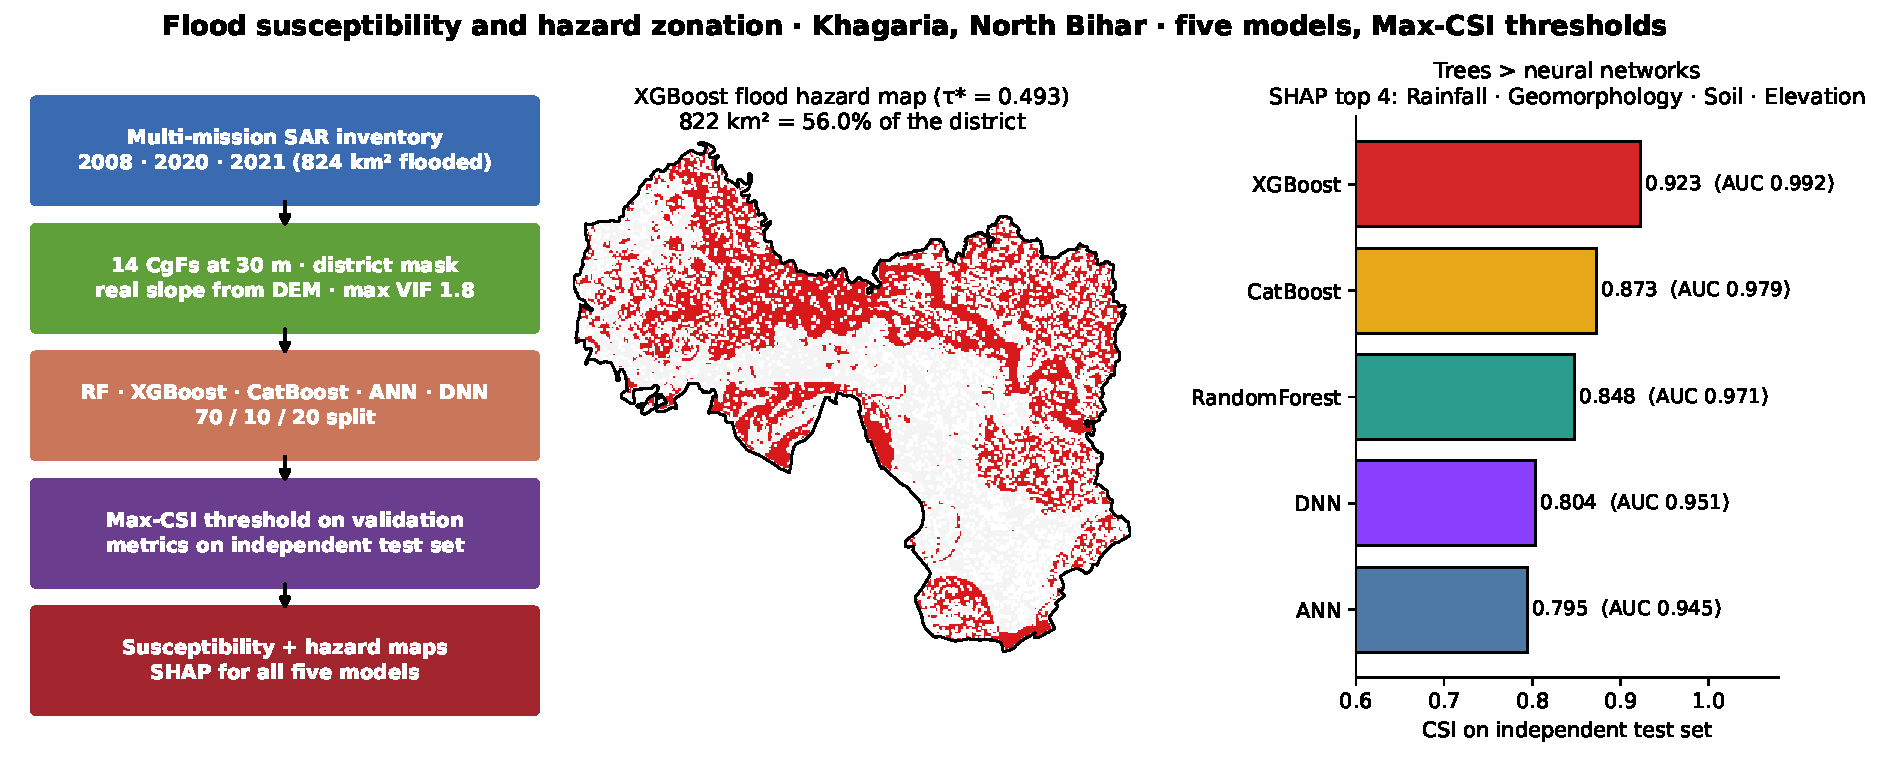
\includegraphics[width=\textwidth]{Figures_v2/Graphical_Abstract.pdf}
    \caption*{\textbf{Graphical Abstract.} Study overview: multi-mission SAR inventory and fourteen CgFs at 30 m, five-model comparison with Max-CSI thresholds chosen on a validation split, the XGBoost binary FHM for Khagaria district, and test-set CSI and AUC for all five models.}
\end{figure}

\newpage

%% ============================================================
%%  1. INTRODUCTION
%% ============================================================
\section{Introduction}

Floods are the most spatially extensive and socially disruptive of all natural hazards, responsible for approximately 40\% of all disaster events globally and disproportionately affecting densely populated alluvial environments \citep{dartmouth2023, wmo2020, UNDRR2020}. During 2000--2019, floods killed over 100,000 people and affected 1.65 billion, with losses concentrated in monsoon-driven Asian river systems \citep{UNDRR2020}. In South Asia, where the Indo-Gangetic Plain concentrates hundreds of millions of people in low-lying terrain drained by glacier-fed Himalayan rivers, this exposure reaches its most acute expression. Bihar state alone sees nearly 73\% of its geographical area --- roughly 68,800 km\textsuperscript{2} --- exposed to recurrent inundation \citep{fmiscwrd2024, ray2019}, with average annual flood losses exceeding 12 billion INR over the past two decades \citep{beams2024}. The annual flood cycle is driven by the synchronised peak discharge of the Ganga and its northern tributaries --- the Kosi, Gandak, Burhi Gandak, Bagmati, and Kamla Balan --- whose origins in the geologically young and tectonically active Himalayas deliver exceptional sediment loads onto a near-flat alluvial plain \citep{gajre2017, sinha2008}. Bed aggradation, channel braiding, and frequent avulsions, compounded by engineering embankments that impede natural drainage and concentrate breach risk, render North Bihar among the most persistently flood-affected regions on Earth \citep{beams2024, mishra2018, Jha2012}. Anthropogenic climate change is further intensifying South Asian Monsoon variability and extreme precipitation frequency \citep{ipcc2021, Singh2022, Mishra2020}, making the development of accurate, high-resolution, and operationally actionable flood hazard frameworks an urgent scientific and policy priority.

Classical flood inundation modelling --- principally physics-based hydrodynamic models such as HEC-RAS, MIKE FLOOD, and LISFLOOD-FP --- offers mechanistic rigour but imposes formidable data demands: high-resolution bathymetric surveys, stream gauge networks, and extensive calibration datasets rarely available in data-scarce developing regions \citep{teng2017, neal2021, Bates2010}. These constraints have catalysed the rise of data-driven approaches leveraging satellite remote sensing and geographic information systems (GIS) to derive flood susceptibility estimates from environmental proxies. Early statistical methods --- Frequency Ratio (FR), Weights of Evidence (WoE), and Logistic Regression (LR) --- established the foundational framework of linking terrain-derived conditioning factors (CgFs) to historical flood occurrence inventories \citep{nampak2014, rahmati2016, Chapi2017}. ML successors --- Support Vector Machines \citep{hong2018}, RF \citep{tehrany2014, Pandey2021FrontEarth, Arora2021ANFIS}, and gradient-boosted tree ensembles \citep{chen2016, prokhorenkova2018} --- progressively improved predictive performance through their capacity to model non-linear predictor-response relationships. The contemporary state-of-the-art in geospatial hazard susceptibility is led by XGBoost and CatBoost, which have produced strong results across landslide \citep{Arabameri2021, Iban2022}, gully erosion \citep{zhang2022}, and flood mapping applications \citep{wang2020, li2021, Nguyen2022, Costache2022, Pourghasemi2020, Arora2025SciRep, Arora2022SERRA, Arora2024Argens}.

In parallel, the broader DL revolution has prompted increasing adoption of Artificial Neural Network (ANN) and Deep Neural Network (DNN) architectures for hydrological modelling and flood prediction, motivated by their theoretical capacity to extract hierarchical feature representations from raw input data \citep{sit2020, Hu2019, Mosavi2018, Ahmadlou2020JFRM}. DL models have achieved notable successes in time-series streamflow forecasting \citep{Kratzert2018, Shen2018}, rainfall--runoff modelling \citep{Frame2022}, and large-scale numerical weather prediction \citep{Bi2023, Lam2023, Rasp2021}, where the temporal continuity, high dimensionality, and volume of training data play directly to the strengths of recurrent and Transformer architectures. In hydrological nowcasting and medium-range weather forecasting, DL models have even begun challenging numerical weather prediction systems built over decades of physics-based development \citep{Bi2023, Lam2023}. These successes have led to a widespread but imprecise assumption that DL represents a universal improvement over classical ML in hydrology --- an assumption that does not hold when the task involves structured, low-dimensional tabular data.

Flood susceptibility mapping is fundamentally a tabular classification problem: each training sample is a pixel described by a finite row of terrain-derived attributes. In this structural setting, a body of rigorous benchmark evidence demonstrates that tree-based ensemble methods consistently outperform DL. \citet{grinsztajn2022} evaluated 45 diverse tabular datasets and found tree-based models retained a decisive advantage, attributing this to their superior inductive bias for the irregular, non-smooth, axis-aligned decision boundaries that characterise structured environmental data --- boundaries fundamentally different from the smooth manifolds that neural networks are biased towards learning. \citet{shwartzziv2022} corroborated this, arguing that DL requires dataset scales rarely attained in district-level geospatial inventories to overcome these architectural disadvantages. \citet{mcelfresh2023} extended the analysis to 176 datasets and reached the same conclusion: no DL architecture consistently dominates tree ensembles on tabular tasks. The physical rationale is transparent: flood susceptibility in alluvial terrain is governed by threshold-type rules operating in feature space --- a pixel floods if its elevation falls below a critical value AND its proximity to a river is within a threshold distance AND local drainage is impeded. These axis-aligned conditions are precisely what recursive binary partitioning in decision trees is designed to represent \citep{breiman2001, Popov2021}. Neural networks, applying stacked linear transformations with smooth activations, impose a prior favouring smooth decision surfaces --- a prior structurally mismatched to the step-wise physical logic of alluvial flood inundation. Calibration is a separate question: neural networks and boosted trees can each produce poorly calibrated probabilities \citep{Niculescu-Mizil2005, zadrozny2002}, so this study reports calibration alongside discrimination rather than inferring it from the position of the optimal threshold.

A related and underexplored methodological gap in the flood mapping literature concerns the transition from continuous susceptibility probability maps to operationally deployable binary flood hazard maps (FHMs). Most studies apply a fixed 0.5 probability cut-off or Youden's Index \citep{youden1950} without accounting for the asymmetric error costs of flood detection, where missed flood zones (false negatives) carry far greater societal consequences --- in terms of loss of life, displacement, and infrastructure damage --- than unnecessary hazard designations (false positives). The Critical Success Index (CSI) --- also known as the Threat Score, originally formalised for severe weather warning verification \citep{schaefer1990} --- simultaneously penalises all three error types (TP, FP, FN) and does not reward true negatives, making it uniquely suited to operational flood mapping in environments where the non-flood class dominates by area \citep{mason2003, Pham2021, nguyen2021}. Despite this suitability, comparative evaluations of threshold optimisation methods for flood hazard zonation remain scarce. The present study operationalises Max-CSI as the primary thresholding criterion and benchmarks it rigorously against Youden's Index across all five models.

The flood inventory underpinning this study was constructed by integrating multi-year SAR-derived flood extents from the 2008, 2020, and 2021 monsoon events in Khagaria district --- an approach that captures the multi-event flood envelope rather than a single-season snapshot, following the multi-temporal inventory framework validated for the Lower Kosi River Basin \citep{Arora2022SERRA}. Sentinel-1 Synthetic Aperture Radar (SAR) imagery in C-band, available through the Copernicus Programme, enables reliable water surface detection through cloud cover and rain-band obscuration during peak monsoon inundation \citep{Twele2016, DeVries2020, dasgupta2018} --- conditions that render optical sensors operationally non-functional.

This study addresses these interconnected gaps through a systematic multi-model comparative analysis of flood susceptibility mapping and FHM derivation in Khagaria district, Bihar --- a district that, despite its extraordinary and well-documented flood exposure at the convergence of seven major river systems, has not been the subject of a rigorous pixel-level ML susceptibility study integrating both tree-based ensembles and DL architectures with a principled threshold optimisation framework. Specifically, the study: (i) constructs a fourteen-CgF geospatial database integrating a multi-year Sentinel-1 SAR-derived flood inventory with terrain, land cover, hydrological, and geological predictors; (ii) screens the factors for collinearity with the Variance Inflation Factor; (iii) trains RF, XGBoost, CatBoost, ANN, and DNN under one pipeline with a train / validation / test split, so that early stopping and thresholds never see the test pixels; (iv) applies SHapley Additive exPlanations (SHAP) to quantify conditioning factor importance across all five models;  (v) derives binary FHMs using Max-CSI threshold optimisation and compares performance against Youden's Index; and (vi) produces pixel-level flood hazard zonation at 30 m resolution to support the DDMA of Khagaria in operational preparedness and mitigation planning.

%% ============================================================
%%  2. STUDY AREA
%% ============================================================
\section{Study Area}

\subsection{Geographical Setting and Topography}

Khagaria district is situated in the heart of North Bihar, spanning latitudes 25\textdegree15'N to 25\textdegree44'N and longitudes 86\textdegree17'E to 86\textdegree52'E (Figure~\ref{fig:study_area}). The district encompasses approximately 1,486 km\textsuperscript{2} and is administratively part of the Munger Division, bounded by Saharsa and Madhepura to the north, Bhagalpur and Munger to the south, Begusarai and Samastipur to the west, and Katihar to the east \citep{khagdist2024}. The topography is quintessential of the Gangetic deltaic plains --- flat, low-lying, and devoid of significant relief. District elevations span approximately 36 m to 47 m above mean sea level, declining gently from north-northwest towards south-southeast --- a characteristic gradient of the Gangetic alluvial plain that severely limits natural drainage capacity \citep{khagdist2024}. This subdued topography constrains drainage efficiency and facilitates stagnation and prolonged recession of floodwaters. Soils are predominantly fine-textured alluvial deposits --- silty clay loams and silty loams --- with low infiltration capacity, exacerbating surface runoff and inundation \citep{NBSSLUPbihar2020}.

\subsection{The District of Seven Rivers}

Khagaria's hydrological identity is defined by its status as the convergence zone for seven major river systems, justifying its epithet as the ``drainage sink of North Bihar'':

\begin{itemize}
    \item \textbf{The Ganga:} The master drain, forming the district's southern boundary. Its elevated stage during monsoon peak acts as a hydraulic barrier, impeding tributary discharge and generating severe drainage congestion --- locally termed \textit{paani band} \citep{beams2024}.
    \item \textbf{The Kosi (Saptakoshi):} Known historically as the ``Sorrow of Bihar,'' the Kosi is notorious for exceptionally high bedload sediment flux and geologically recent mega-avulsions, having shifted approximately 120 km westward over roughly two-and-a-half centuries through repeated avulsion cycles \citep{sinha2008, mishra2018}. The Kosi carries approximately 100--150 million tonnes of sediment annually, progressively raising its bed above the surrounding floodplain and increasing avulsion risk \citep{sinha2008}.
    \item \textbf{The Burhi Gandak:} A meandering river joining the Ganga near Gogri Jamalpur; embankment breaches are a recurrent cause of inundation, particularly in Gogri and Mansi blocks.
    \item \textbf{The Bagmati and Kamla Balan:} Himalayan tributaries with flashy regimes, high suspended sediment loads, and documented susceptibility to embankment breaching during sustained high-discharge episodes \citep{mishra2018}.
    \item \textbf{The Kareh and Kali Kosi:} Significant distributary channels contributing to peripheral block inundation in Alauli, Beldaur, and Parbatta blocks.
\end{itemize}

The convergence of these systems within a single low-lying district means that multiple rivers may peak simultaneously, preventing drainage of any individual channel and producing multi-week inundation episodes. The \textit{chaur} depressions --- oxbow-lake remnants and shallow inter-levee basins scattered throughout the district --- act as secondary water retention zones and experience the most prolonged flooding.

\subsection{Climate and Flood History}

Khagaria experiences a humid subtropical climate (K\"{o}ppen: Cwa). The Southwest Monsoon (June--September) delivers approximately 1,255 mm annually with high inter-annual variability \citep{beams2024}. Historically significant events include the 1987 Kosi dam-burst (damages exceeding 68 billion INR), the 2004 Bagmati-Kamla flood, the catastrophic 2008 Kosi course-change near Kusaha, Nepal --- which shifted the river approximately 120 km eastward in days and inundated over 3,400 km\textsuperscript{2} of Bihar \citep{bhuvan2010, mishra2018} --- and the 2024 double-peak inundation associated with cyclonic-monsoon interactions \citep{tatatrusts2024}. The union of the 2008, 2020, and 2021 SAR flood extents used as the inventory in this study covers 824.4 km\textsuperscript{2} of the modelled district area (Figure~\ref{fig:study_area}).

\begin{figure}[H]
    \centering
    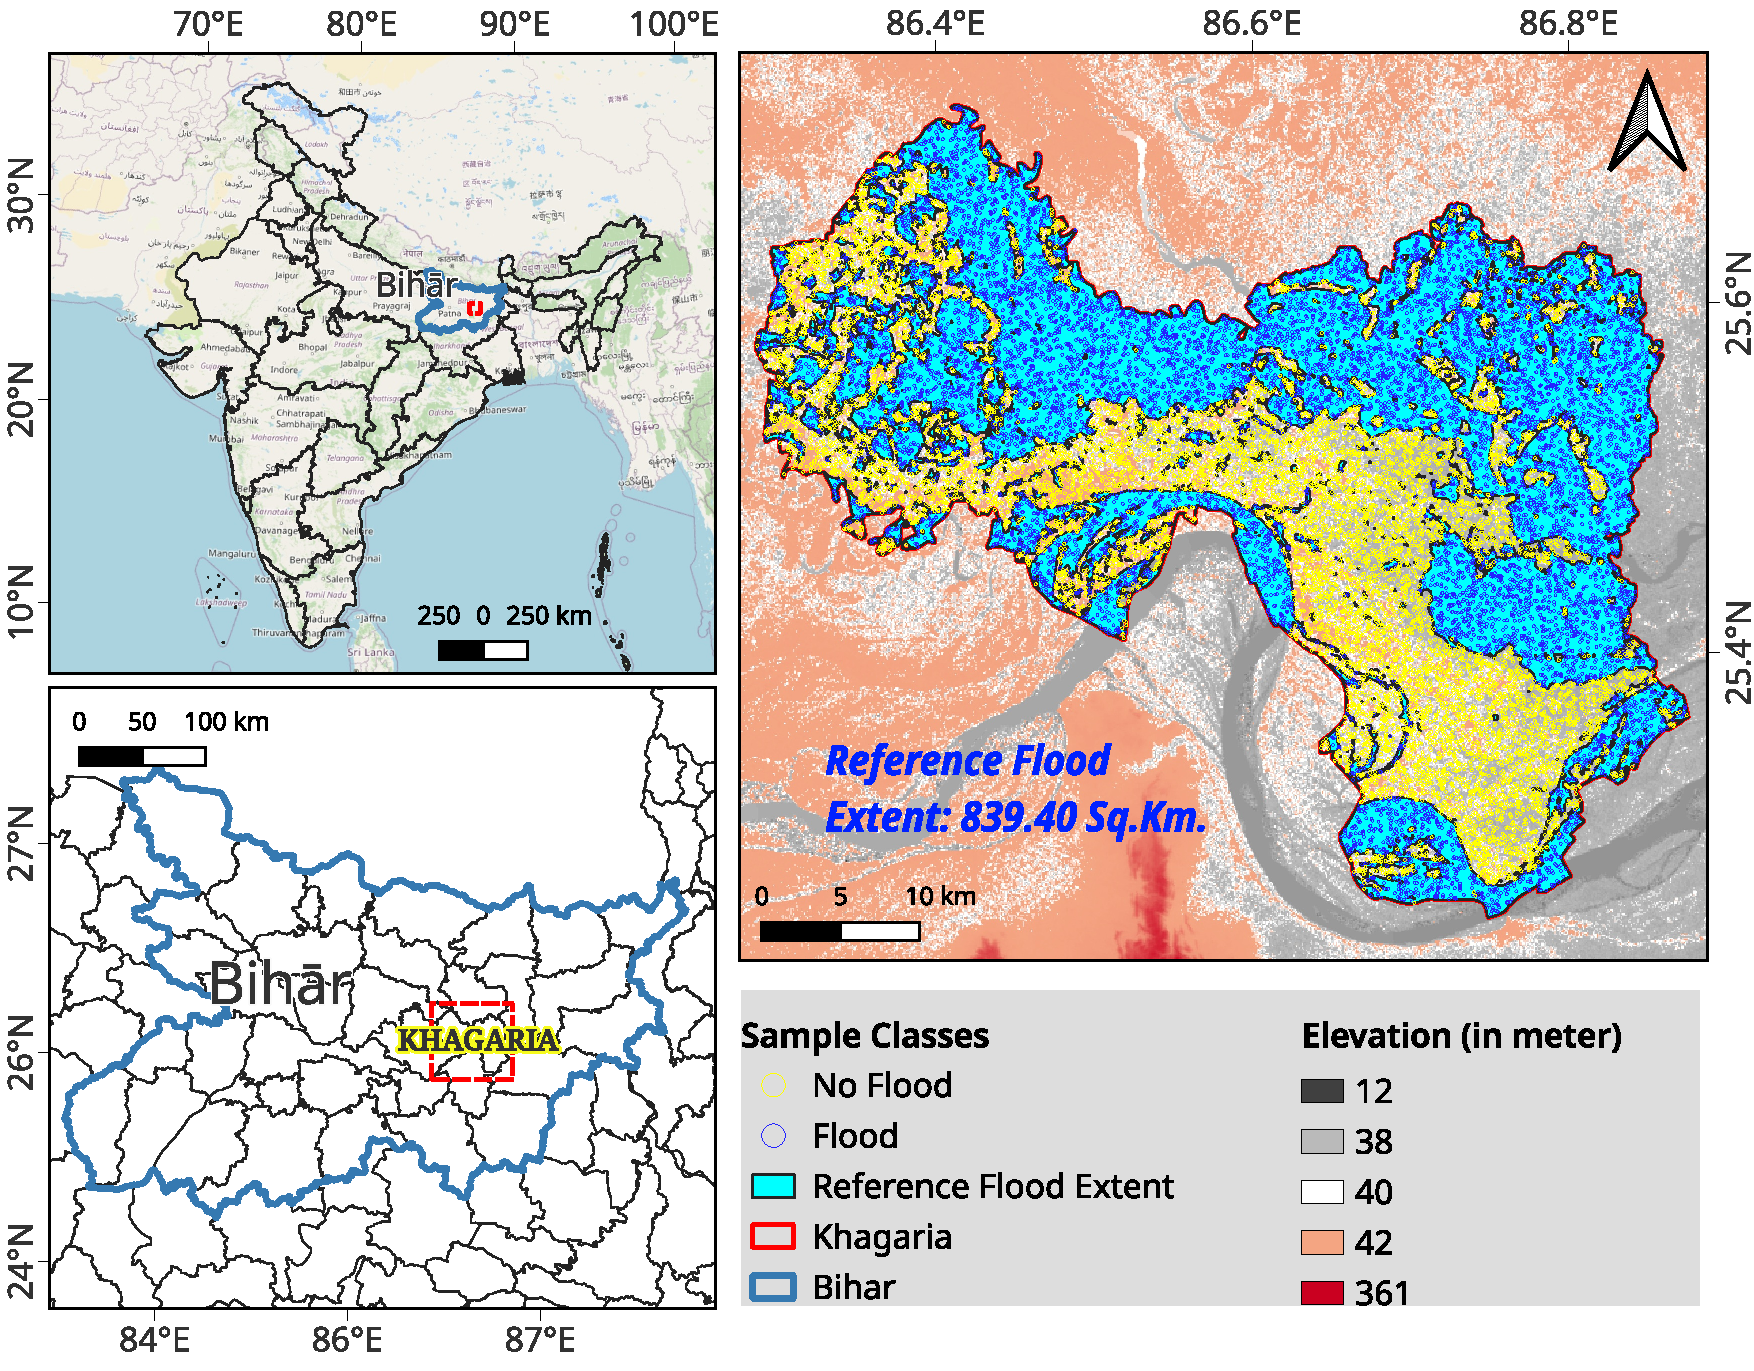
\includegraphics[width=\textwidth]{Figures/Location_map.pdf}
    \caption{Study area: Khagaria district, North Bihar, India. (Left panels) Bihar within India and Khagaria within Bihar; (Right) district boundary with block boundaries, seven major river systems, and the spatial distribution of the multi-year Sentinel-1 SAR-derived flood and non-flood inventory samples overlaid on an elevation-based background. The reference flood extent (824.4 km\textsuperscript{2} inside the modelled district area) is shown in cyan. The district occupies the hydrological sink of North Bihar, receiving simultaneous peak discharge from the Kosi, Bagmati, Burhi Gandak, and other tributaries before their confluence with the Ganga.}
    \label{fig:study_area}
\end{figure}

%% ============================================================
%%  3. MATERIALS AND METHODS
%% ============================================================
\section{Materials and Methods}

The methodological workflow comprises six sequential phases: (1) flood inventory construction from multi-year SAR, (2) CgF preparation, district masking, and spatial alignment, (3) multi-collinearity analysis via VIF, (4) model training with a train / validation / test split, (5) spatial susceptibility prediction, and (6) threshold-optimised FHM derivation (Figure~\ref{fig:workflow}).

\begin{figure}[H]
    \centering
    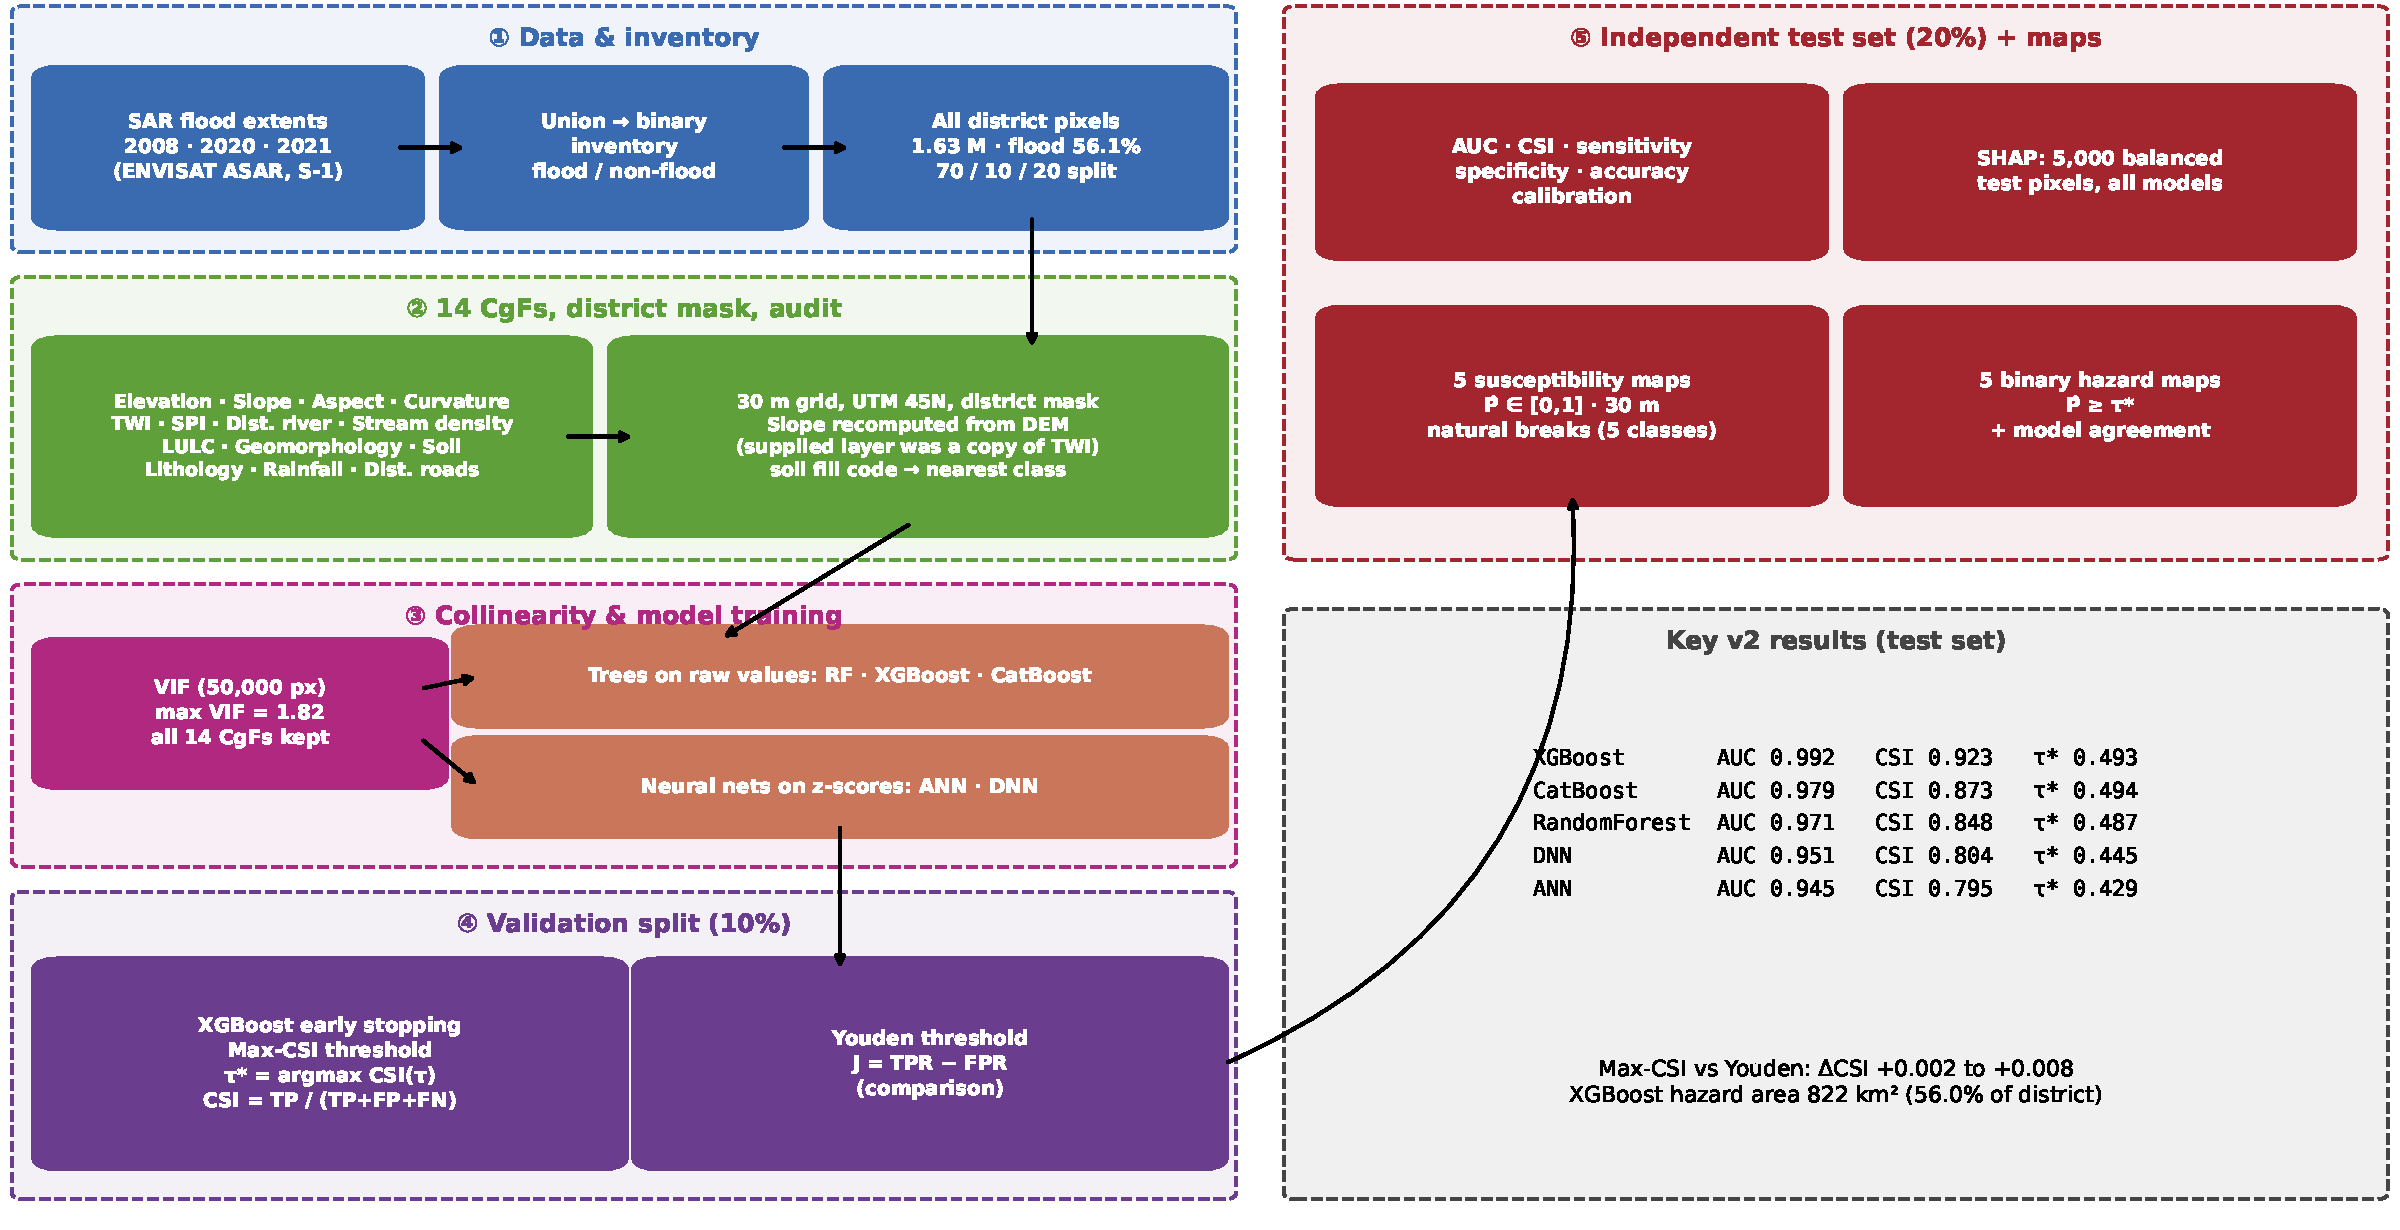
\includegraphics[width=\textwidth]{Figures_v2/FHM_Khagaria_Methodology_Flowchart.pdf}
    \caption{Methodological workflow. All five models use the same fourteen CgFs (tree models on raw values, neural networks on standardised values). Early stopping and both thresholds (Max-CSI, Youden) are chosen on the validation split; all reported metrics are computed on the independent test split.}
    \label{fig:workflow}
\end{figure}

\subsection{Flood Inventory: Ground Truth Construction}

The dependent variable is a binary flood inventory raster classifying each pixel as Flood (1) or Non-Flood (0). The inventory was constructed by integrating SAR-derived flood extents from three major flood events in Khagaria: the 2008 Kosi avulsion flood, and the 2020 and 2021 monsoon peak inundation episodes. This multi-year integration approach captures the full spatial envelope of flood occurrence rather than a single-event snapshot, following the methodology validated for the Lower Kosi River Basin \citep{Arora2022SERRA}.

SAR imagery from two sensor missions was acquired during peak flood episodes to build the multi-temporal inventory. For the 2008 Kosi avulsion event, ENVISAT ASAR Wide Swath Mode (WSM) scenes were used, providing C-band backscatter at approximately 150 m native resolution resampled to 30 m \citep{Twele2016}; the 2008 dataset constitutes the most important inventory event given the exceptional spatial extent of that avulsion. For the 2020 and 2021 monsoon peak inundations, Sentinel-1A/B Ground Range Detected (GRD) IW-mode imagery (C-band, 5.405 GHz; VV polarisation; 10 m native, resampled to 30 m) was used \citep{DeVries2020, dasgupta2018}. SAR imagery was preferred over optical sensors for its capability to penetrate persistent cloud cover and monsoon rain-band obscuration that renders optical data non-functional during peak inundation \citep{srivastava2017}. Open water exhibits distinctly lower backscatter than vegetated or built-up surfaces due to specular reflection, enabling reliable water/non-water discrimination via threshold-based change-detection \citep{bauer2015, Twele2016}. Single-event binary flood masks were produced independently for each year and merged by spatial union at the 30 m grid, so that the inventory represents the maximum observed inundation extent rather than any single event \citep{Arora2022SERRA}. Every pixel of the district is labelled: pixels flooded in any of the three events are Flood (1) and all other pixels are Non-Flood (0). Of the 1,632,234 valid district pixels (1,469.0 km\textsuperscript{2}), 915,986 (824.4 km\textsuperscript{2}; 56.1\%) are flooded, so the classes are close to balanced and no resampling was applied. The pixels were split by stratified random sampling (seed 42) into training, validation, and test sets:
\begin{equation}
    \text{Training} = 70\%\ (1{,}142{,}563),\quad \text{Validation} = 10\%\ (163{,}224),\quad \text{Test} = 20\%\ (326{,}447)
\end{equation}
The validation set is used only for XGBoost early stopping and for choosing thresholds; the test set is used only for the reported metrics.

\subsection{Flood Conditioning Factors}

Fourteen CgFs were selected based on a systematic literature review of flood susceptibility modelling \citep{khosravi2018, tehrany2019, rahmati2016, Costache2022, Pourghasemi2020, Pandey2021FrontEarth, Arora2022SERRA} and the physico-geographic characteristics of Khagaria's alluvial environment (Table~\ref{tab:factors}). The selection spans five thematic domains: topographic controls (Elevation, Slope, Curvature, Aspect, TWI, SPI), hydrological proximity (Distance to River, Stream Density), land surface characteristics (LULC, Geomorphology, Soil), geological substrate (Lithology), climatic forcing (Rainfall), and anthropogenic drainage modification (Distance to Roads). All CgFs were prepared as GeoTIFF rasters aligned to a common reference grid at 30 m spatial resolution.

\begin{table}[H]
\centering
\caption{Flood conditioning factors (CgFs) employed in this study.}
\label{tab:factors}
\small
\begin{tabularx}{\linewidth}{@{} c l l X @{}}
\toprule
\textbf{No.} & \textbf{Factor} & \textbf{Source} & \textbf{Hydrological Rationale} \\
\midrule
1  & Aspect              & Derived (SRTM)            & Directional exposure influences moisture and evapotranspiration \\
2  & Curvature           & Derived (SRTM)            & Identifies concave surfaces as water collection zones \\
3  & Distance to River   & Derived (SRTM)            & Proximity increases exposure to bank overflow \\
4  & Distance to Roads   & OSM                       & Road embankments alter local drainage patterns \\
5  & Elevation           & SRTM 30 m                 & Primary control on inundation depth and extent \\
6  & Geomorphology       & GSI                       & Floodplain geomorphological unit classification \\
7  & Lithology           & GSI                       & Bedrock type influences groundwater dynamics and permeability \\
8  & LULC                & Sentinel-2                & Vegetation and impervious cover modulate infiltration \\
9  & Rainfall            & IMD Gridded (1901-2021)   & Primary triggering factor for surface runoff generation \\
10 & Slope               & Derived (SRTM)            & Controls overland flow velocity; near-zero slopes intensify ponding \\
11 & Soil                & HWSD, FAO                 & Controls infiltration rate and hydraulic conductivity \\
12 & Stream Density      & Derived (SRTM)            & Dense networks accelerate runoff concentration \\
13 & Stream Power Index  & Derived (SRTM)            & Measures erosive power of overland flow \\
14 & TWI                 & Derived (SRTM)            & Quantifies soil saturation propensity and flow accumulation \\
\bottomrule
\end{tabularx}
\end{table}

\subsection{Data Preprocessing and Spatial Alignment}

All CgF rasters were reprojected to UTM Zone 45N (WGS84) on a common 30 m grid using nearest-neighbour resampling via \texttt{rasterio.warp.reproject()} \citep{gillies2019}. Pixels outside the district boundary, or with a missing value in any CgF, were excluded from training and prediction:
\begin{equation}
    \text{mask}_{i} = \bigcap_{k=1}^{K}\Big[\big(\text{value}_{k,i} \neq \text{NoData}_k\big) \cap \big(\neg\,\text{NaN}_{k,i}\big)\Big]
\end{equation}
where $i$ indexes pixels and $k$ indexes layers. An audit of the input layers led to two corrections before training. First, Slope was recomputed from the SRTM elevation grid with Horn's 3$\times$3 method, because the supplied slope layer was found to be a copy of the TWI layer. Over the district, the recomputed slope has a mean of 1.8\textdegree{} and a 99th percentile of 6.0\textdegree; in this flat terrain these values are dominated by the 1 m vertical quantisation and noise of SRTM rather than by real relief. Second, 17,803 district pixels (1.1\%) carried the Soil fill code (65,535) instead of a soil class; each was assigned the nearest valid soil class. Neural network architectures additionally require normalised inputs for stable gradient descent \citep{lecun2012, Goodfellow2016}; all features were scaled using zero-mean, unit-variance standardisation:
\begin{equation}
    x' = \frac{x - \mu}{\sigma}
\end{equation}
where $\mu$ and $\sigma$ are training-set statistics applied unchanged to the validation and test sets and to the full prediction rasters. Tree-based models were trained on raw (unscaled) values, as they are invariant to monotonic transformations \citep{breiman2001}. The categorical factors (Geomorphology, Lithology, LULC, Soil) enter all models as integer class codes.

\subsection{Multi-Collinearity Analysis: Variance Inflation Factor}

Multi-collinearity among predictor variables can destabilise neural network gradient descent and inflate prediction variance \citep{dormann2013, Belsley2005}. The VIF was computed for each CgF:
\begin{equation}
    \text{VIF}_{j} = \frac{1}{1 - R^{2}_{j}}
\end{equation}
where $R^{2}_{j}$ is the coefficient of determination from regressing the $j^{\text{th}}$ predictor on all remaining predictors. VIF was computed from the correlation matrix of a random subsample of 50,000 training pixels, with a threshold of 10 \citep{dormann2013, OBrien2007}; any factor above the threshold would be removed from the ANN and DNN inputs only, since tree ensembles are insensitive to collinearity. Slope and TWI are related through the TWI definition,
\begin{equation}
    \text{TWI} = \ln\left(\frac{A_s}{\tan \beta}\right)
\end{equation}
where $A_s$ is the specific catchment area and $\beta$ is local slope angle, but the contributing-area term keeps the two from being collinear in practice (Section~\ref{sec:res_vif}).

\begin{figure}[H]
    \centering
    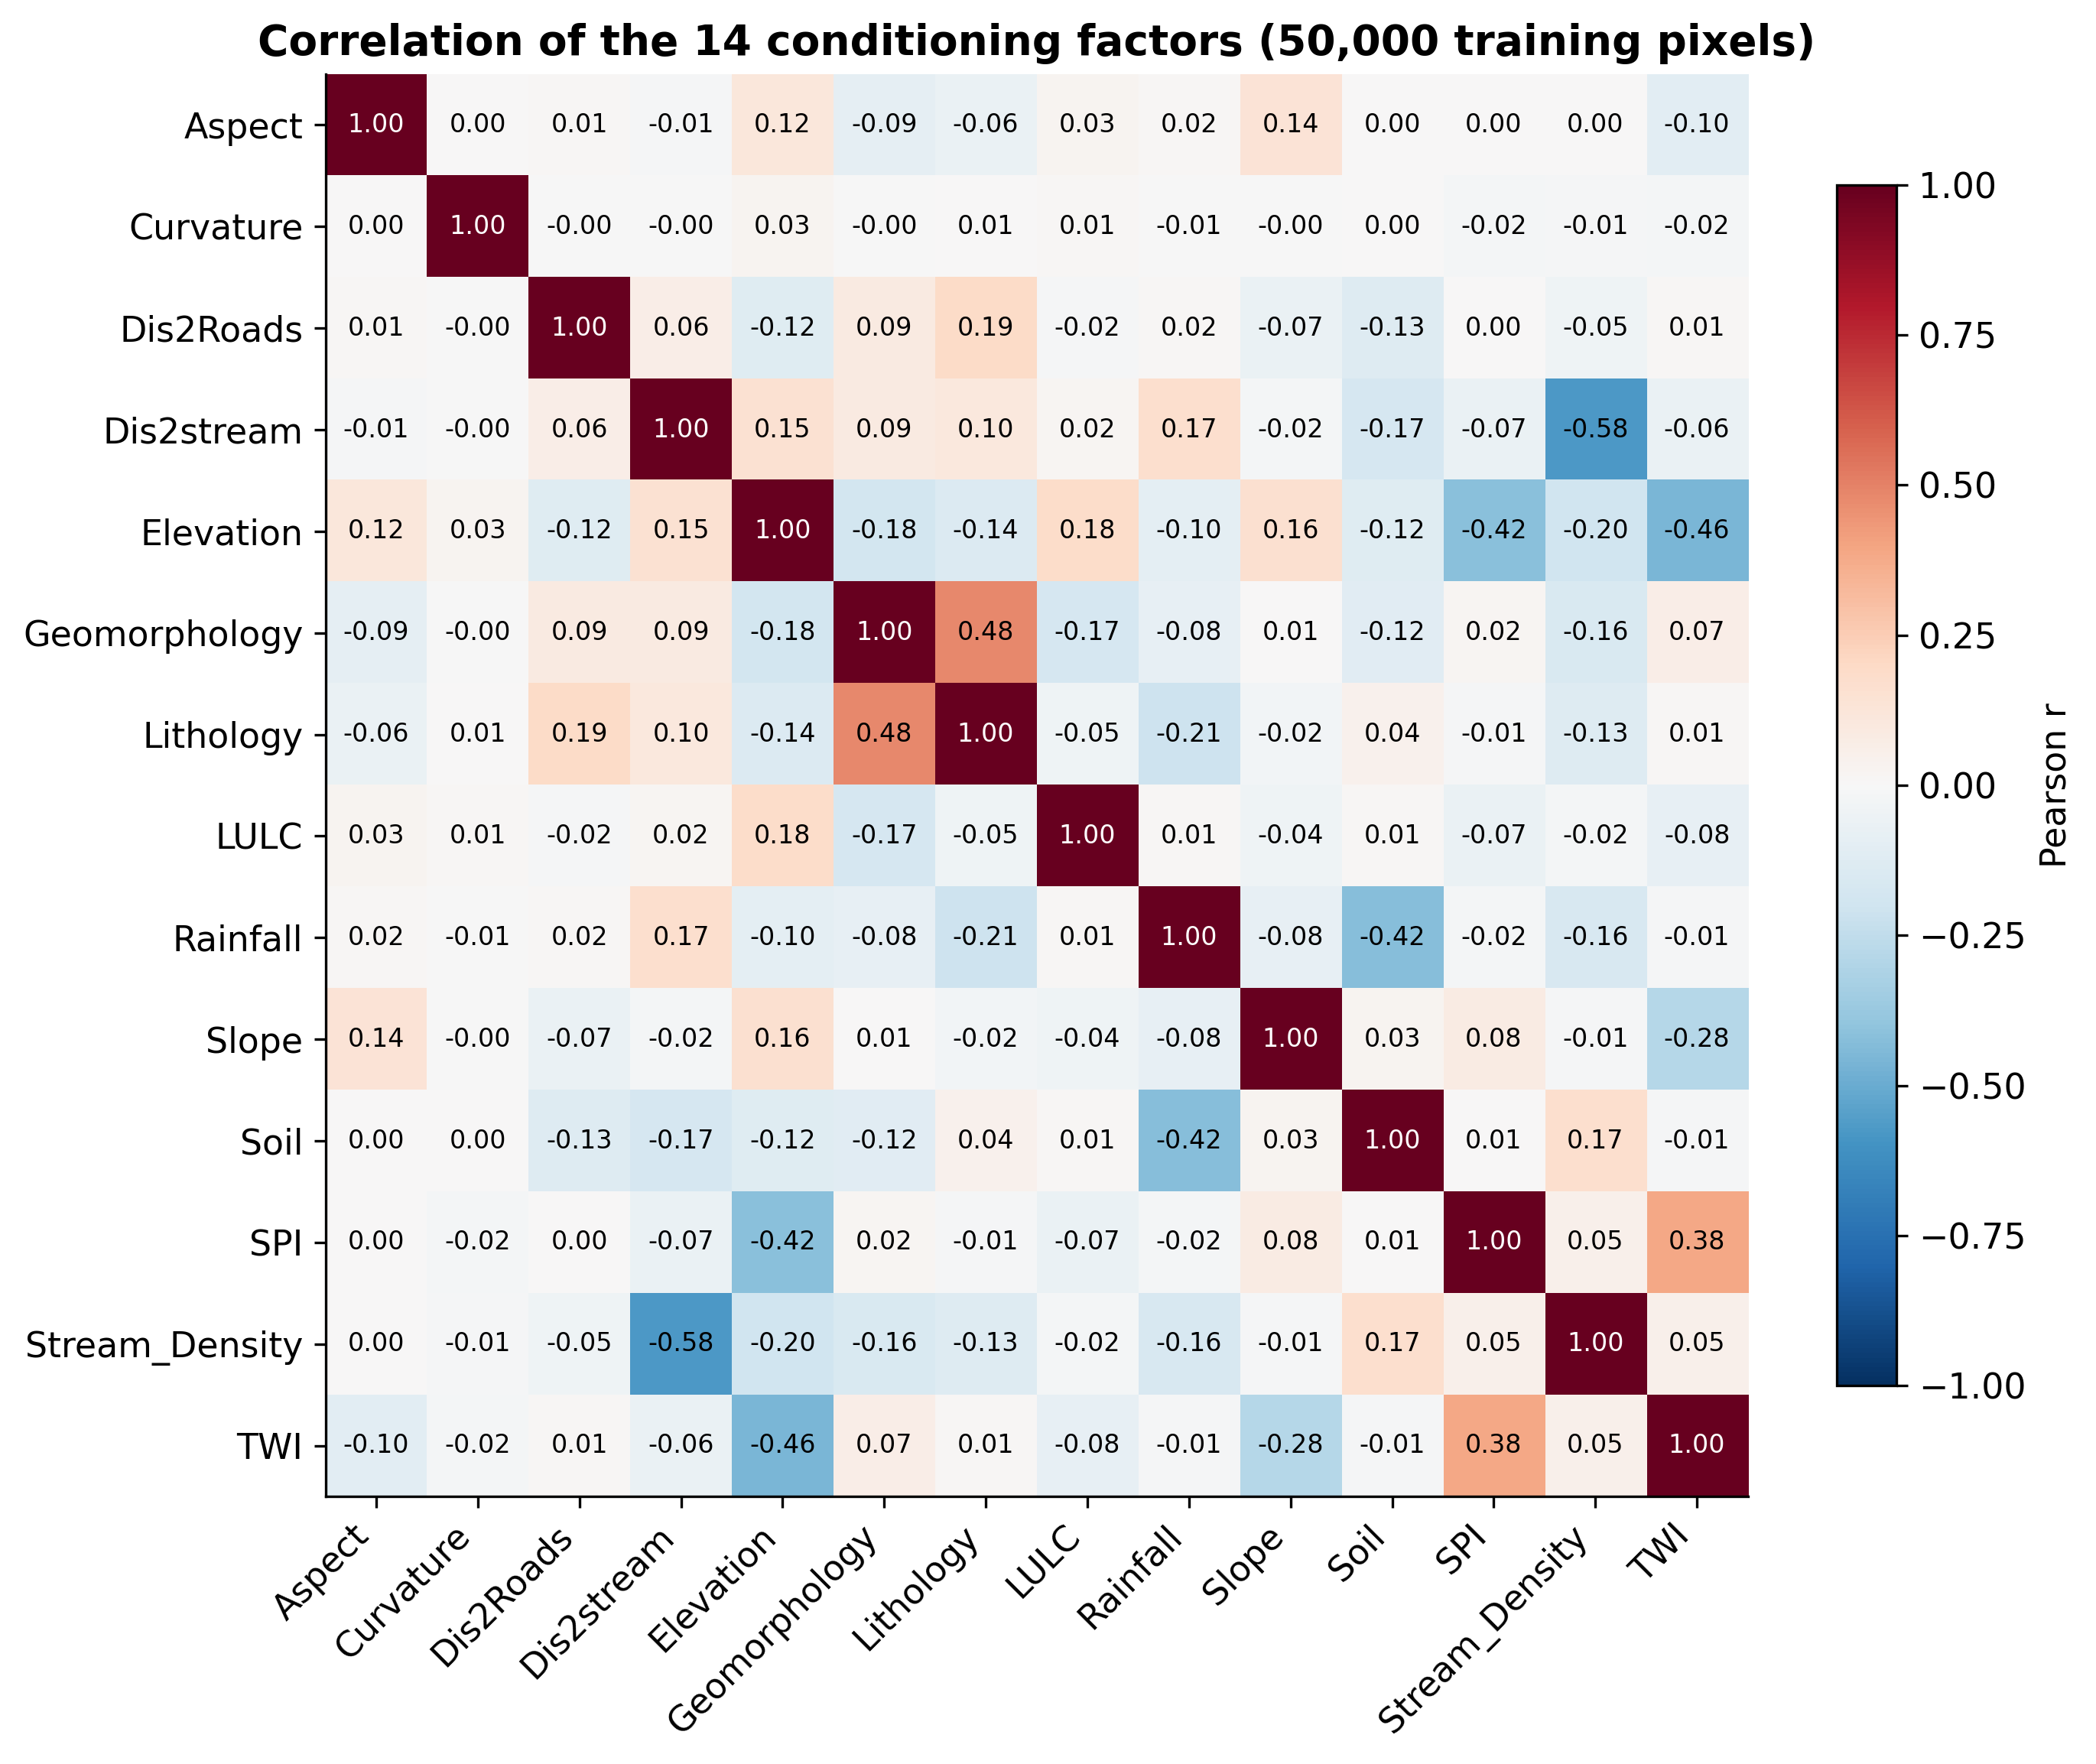
\includegraphics[width=0.95\textwidth]{Figures_v2/Correlation_Matrix_Robust.png}
    \caption{Pearson correlation matrix for the fourteen CgFs computed from 50,000 training pixels. The strongest correlations are between Distance to Stream and Stream Density ($r = -0.58$), Geomorphology and Lithology ($r = 0.48$), Elevation and TWI ($r = -0.46$), Rainfall and Soil ($r = -0.42$), and Elevation and SPI ($r = -0.42$). Slope and TWI are only weakly correlated ($r = -0.28$).}
    \label{fig:corrmatrix}
\end{figure}

\subsection{Model Architectures and Training}

\subsubsection{Random Forest}
RF is a bagging ensemble constructing $T$ independent decision trees, each trained on a bootstrap resample using a random subset of $\sqrt{p}$ features at each split node \citep{breiman2001, belgiu2016}. Predictions are averaged probability estimates across all trees. The scikit-learn implementation was used with $T = 150$ trees and maximum depth of 16, on all 14 raw CgFs.

\subsubsection{XGBoost}
XGBoost \citep{chen2016} constructs an additive ensemble of decision trees sequentially, each fitted to the negative gradient of a regularised second-order Taylor expansion of the loss:
\begin{equation}
    \mathcal{L}^{(t)} \approx \sum_{i=1}^{n} \left[g_i f_t(x_i) + \frac{1}{2}h_i f_t^2(x_i)\right] + \Omega(f_t)
\end{equation}
where $g_i$ and $h_i$ are the first and second derivatives of the loss, and $\Omega(f_t)$ penalises tree complexity via $L_1$ and $L_2$ regularisation. Hyperparameters: maximum depth = 8, learning rate = 0.1, subsample = 0.8, up to 1,000 boosting rounds with early stopping on the validation set (20 rounds without AUC improvement), histogram tree method. Validation AUC was still improving at round 1,000, so all 1,000 rounds were kept (Figure~\ref{fig:training_curves}).

\subsubsection{CatBoost}
CatBoost \citep{prokhorenkova2018} introduces two algorithmic innovations: (i) \textit{Ordered Boosting}, using a random permutation to compute unbiased gradient estimates and mitigate target leakage; and (ii) \textit{Oblivious Trees} (symmetric decision trees), applying the same split at all nodes of a given depth level for efficient and regularised inference \citep{Dorogush2018}. Training: 800 iterations, learning rate 0.1, depth 8.

\subsubsection{Artificial Neural Network}
The ANN employed a shallow feed-forward topology trained on all 14 standardised CgFs:
\begin{multline}
    \text{Input}(p) \to \text{Linear}(64) \to \text{ReLU} \to \text{BatchNorm} \to \text{Dropout}(0.3) \\
    \to \text{Linear}(32) \to \text{ReLU} \to \text{Linear}(1) \to \sigma
\end{multline}
where $\sigma$ is the sigmoid activation and $p = 14$. Batch normalisation and dropout serve as regularisation against overfitting \citep{ioffe2015, srivastava2014}. Loss: Binary Cross-Entropy with Logits; optimisation: Adam \citep{kingma2014}, learning rate $10^{-3}$, 15 epochs, batch size 4,096. Implemented in PyTorch \citep{paszke2019}. Training and validation losses per epoch are shown in Figure~\ref{fig:training_curves}.

\subsubsection{Deep Neural Network}
The DNN extended the ANN by increasing depth:
\begin{multline}
    \text{Input}(p) \to \text{Linear}(128) \to \text{ReLU} \to \text{BN} \to \text{Drop}(0.4) \to \text{Linear}(64) \\
    \to \text{ReLU} \to \text{BN} \to \text{Drop}(0.3) \to \text{Linear}(32) \to \text{ReLU} \to \text{Linear}(1) \to \sigma
\end{multline}
The deeper architecture theoretically enables hierarchical feature abstraction but, as the results demonstrate, confers no performance advantage over tree ensembles for this tabular dataset \citep{grinsztajn2022, shwartzziv2022}. The same training configuration as the ANN was applied: Adam, $\text{lr} = 10^{-3}$, 15 epochs, batch size 4,096.

\subsection{SHAP Explainability Analysis}
\label{sec:shap_method}

To provide model-conditioned, physically interpretable importance scores, SHAP \citep{lundberg2017, lundberg2020} were computed post-training for all five models. SHAP uniquely satisfies the four Shapley axioms --- efficiency, symmetry, linearity, and dummy \citep{shapley1953} --- guaranteeing a fair attribution of each prediction to each input feature that is both theoretically sound and locally accurate.

\subsubsection{SHAP Computation per Model Type}

\begin{description}[style=nextline, align=left]
  \item[\textbf{XGBoost:}] Exact TreeSHAP via \texttt{booster.predict(pred\_contribs=True)}, XGBoost's native SHAP path; the last (bias) column is discarded.

  \item[\textbf{CatBoost:}] Exact Shapley values via \texttt{model.get\_feature\_importance(data=pool, type=`ShapValues')}.

  \item[\textbf{RandomForest:}] \texttt{shap.TreeExplainer} \citep{lundberg2020} applied to the trained 150-tree forest itself.

  \item[\textbf{ANN and DNN:}] \texttt{shap.GradientExplainer} (expected gradients, an extension of Integrated Gradients \citep{Sundararajan2017}) with 500 training pixels as background.
\end{description}

SHAP values were computed on a balanced sample of $N = 5{,}000$ test pixels ($2{,}500$ flood; $2{,}500$ non-flood). XGBoost, CatBoost, ANN, and DNN attributions are in log-odds units and RF attributions in probability units, so mean absolute SHAP values $\bar{|\phi_j|}$ were min--max normalised to $[0,1]$ within each model before comparison.

\subsection{Spatial Prediction}

Each trained model generated a continuous probability map $\hat{P} \in [0,1]$ for every valid district pixel, constituting the flood susceptibility map (FSM). All outputs were saved as float32 GeoTIFF files with the grid's coordinate reference system and a NoData value outside the district. For visualisation, the continuous FSMs were reclassified into five susceptibility classes using Natural Breaks (Jenks) computed on the XGBoost probability map and applied to all five models: Very Low (0.00--0.12), Low (0.12--0.35), Moderate (0.35--0.64), High (0.64--0.88), and Very High (0.88--1.00).

\subsection{Threshold Optimisation: Maximum Critical Success Index}

Converting continuous FSM probabilities to binary FHMs requires selection of a decision threshold $\tau$. Standard approaches use $\tau = 0.5$ or Youden's Index \citep{youden1950}:
\begin{equation}
    J = \text{Sensitivity} + \text{Specificity} - 1 = \text{TPR} - \text{FPR}
\end{equation}
These are suboptimal for imbalanced flood inventories where false negatives carry asymmetric operational costs. This study adopted Max-CSI \citep{schaefer1990, wilks2019}:
\begin{equation}
    \text{CSI} = \frac{\text{TP}}{\text{TP} + \text{FP} + \text{FN}}
\end{equation}
where TP, FP, and FN denote true positives, false positives, and false negatives. The CSI simultaneously penalises all three error types and does not reward true negatives (safe pixels correctly classified as safe), making it uniquely aligned with the operational objective of flood hazard detection \citep{mason2003, Pham2021}. Given ROC-curve-derived thresholds $\{\tau_k\}$ with corresponding true positive rate (TPR) and false positive rate (FPR), the CSI was computed efficiently via:
\begin{equation}
    \text{CSI}_k = \frac{\text{TPR}_k \cdot P}{P + \text{FPR}_k \cdot N}
\end{equation}
where $P$ and $N$ are the total flood and non-flood pixel counts respectively. The optimal threshold is $\tau^* = \tau_{\arg\max_k \text{CSI}_k}$, and Youden's threshold is $\tau_{\arg\max_k J_k}$. Both thresholds were chosen on the validation set and then applied unchanged to the test set and to the full map. Pixels with $\hat{P} \geq \tau^*$ were classified as Flood Hazard Zone (1); otherwise as Safe Zone (0). The CSI and Youden's J curves across all thresholds, with the test CSI at each chosen threshold, are presented in the Results section (Figure~\ref{fig:maxcsi}).

\subsection{Validation Metrics}

Model performance was assessed on the test set using: (1) AUC --- discrimination ability across all possible thresholds; (2) CSI at $\tau^*$ --- threshold-specific flood detection accuracy penalising FP and FN; (3) Sensitivity (TPR) --- fraction of actual flood pixels correctly identified; (4) Specificity (TNR) --- fraction of safe pixels correctly identified; (5) overall Accuracy; and (6) calibration, summarised by the expected calibration error (ECE) over ten equal-width probability bins \citep{Niculescu-Mizil2005}. These metrics jointly address ranking ability, operational classification performance, and the reliability of the probabilities themselves \citep{Fawcett2006, Powers2011}. Training, validation, and test AUC are reported together to quantify overfitting.

\subsection*{Use of AI Tools}
\textcolor{red}{\textit{[Author note: complete this statement accurately before submission. The October 2026 re-analysis (input audit, retraining, evaluation scripts, figures, and the revised text) was carried out with the assistance of an AI coding assistant (Claude, Anthropic), so the earlier suggested wording ``not used for data analysis'' no longer applies. Suggested wording, to be verified and adjusted: ``An AI assistant (Claude, Anthropic) was used to help write analysis code, audit the input data, and draft and edit parts of the manuscript. All AI-assisted code, results, and text were reviewed and verified by the authors, who take full responsibility for the work.'']}}

%% ============================================================
%%  4. RESULTS
%% ============================================================
\section{Results}

\subsection{Multi-Collinearity Analysis}
\label{sec:res_vif}

No CgF approaches the VIF threshold (Table~\ref{tab:vif}): VIF ranges from 1.001 (Curvature) to 1.821 (Elevation), so all fourteen factors were retained for every model, including the neural networks. Slope (VIF = 1.19) and TWI (VIF = 1.51) are only weakly correlated ($r = -0.28$), because the contributing-area term dominates the TWI in this low-relief terrain. The correlation matrix (Figure~\ref{fig:corrmatrix}) shows a moderate negative correlation between Distance to Stream and Stream Density ($r = -0.58$), consistent with the relationship between channel proximity and drainage density in the Gangetic floodplain. The Geomorphology--Lithology correlation ($r = 0.48$) reflects the co-occurrence of landform units and underlying formations, and the negative correlations of Elevation with TWI ($r = -0.46$) and SPI ($r = -0.42$) are expected because lower-lying areas accumulate flow. Rainfall and Soil are also negatively correlated ($r = -0.42$), as both vary mainly from north to south across the district.

\begin{table}[H]
\centering
\caption{VIF scores for all fourteen CgFs (50,000 training pixels), ordered by VIF value. All factors are below the threshold of 10 and were retained for all five models.}
\label{tab:vif}
\small
\begin{tabular}{lcc}
\toprule
\textbf{Factor} & \textbf{VIF} & \textbf{Feature Set} \\
\midrule
Elevation          & 1.821 & All models \\
Stream Density     & 1.617 & All models \\
Distance to River  & 1.536 & All models \\
TWI                & 1.511 & All models \\
Rainfall           & 1.460 & All models \\
Lithology          & 1.447 & All models \\
Geomorphology      & 1.446 & All models \\
Soil               & 1.392 & All models \\
Stream Power Index & 1.391 & All models \\
Slope              & 1.189 & All models \\
Distance to Roads  & 1.089 & All models \\
LULC               & 1.065 & All models \\
Aspect             & 1.041 & All models \\
Curvature          & 1.001 & All models \\
\bottomrule
\end{tabular}
\end{table}

\subsection{Model Validation and Performance Metrics}

Table~\ref{tab:results} presents the test-set results for all five models at their Max-CSI thresholds. Training, validation, and test AUC are compared in Table~\ref{tab:training}. ROC curves for the training and test sets are shown in Figures~\ref{fig:roc_train} and~\ref{fig:roc_val}, respectively.

\begin{table}[H]
\centering
\caption{AUC on the training (200,000-pixel random subsample), validation, and test sets, and expected calibration error (ECE, ten bins) on the test set.}
\label{tab:training}
\begin{adjustbox}{max width=\linewidth}
\begin{tabular}{lcccc}
\toprule
\textbf{Model} & \textbf{Training AUC} & \textbf{Validation AUC} & \textbf{Test AUC} & \textbf{Test ECE} \\
\midrule
XGBoost       & 0.9966 & 0.9917 & 0.9920 & 0.023 \\
CatBoost      & 0.9803 & 0.9791 & 0.9794 & 0.027 \\
RandomForest  & 0.9774 & 0.9702 & 0.9708 & 0.054 \\
DNN           & 0.9510 & 0.9510 & 0.9511 & 0.013 \\
ANN           & 0.9450 & 0.9449 & 0.9452 & 0.014 \\
\bottomrule
\end{tabular}
\end{adjustbox}
\end{table}

\begin{table}[H]
\centering
\caption{Test-set performance of the five models at their Max-CSI thresholds (chosen on the validation set), ranked by CSI.}
\label{tab:results}
\begin{adjustbox}{max width=\linewidth}
\begin{tabular}{lcccccc}
\toprule
\textbf{Model} & \textbf{AUC} & \textbf{CSI} & \textbf{Sensitivity} & \textbf{Specificity} & \textbf{Accuracy} & \textbf{$\tau^*$} \\
\midrule
XGBoost       & 0.9920 & 0.9229 & 0.9586 & 0.9504 & 0.9550 & 0.493 \\
CatBoost      & 0.9794 & 0.8731 & 0.9320 & 0.9138 & 0.9240 & 0.494 \\
RandomForest  & 0.9708 & 0.8483 & 0.9206 & 0.8911 & 0.9076 & 0.487 \\
DNN           & 0.9511 & 0.8041 & 0.9087 & 0.8336 & 0.8758 & 0.446 \\
ANN           & 0.9452 & 0.7946 & 0.9125 & 0.8102 & 0.8676 & 0.429 \\
\bottomrule
\end{tabular}
\end{adjustbox}
\end{table}

Validation and test AUC agree to within 0.001 for every model, and the gap between training and test AUC is small: 0.005 for XGBoost, 0.007 for RF, 0.001 for CatBoost, and below 0.001 for ANN and DNN. None of the models overfits appreciably, so the lower scores of the neural networks are not an overfitting effect.

XGBoost achieved the highest performance across all metrics (AUC = 0.9920; CSI = 0.9229) at $\tau^* = 0.493$. CatBoost ranked second (AUC = 0.9794; CSI = 0.8731) and RF third (AUC = 0.9708; CSI = 0.8483), consistent with the competitiveness of ensemble methods on tabular geospatial data \citep{belgiu2016, Rodriguez-Galiano2012}. DNN (CSI = 0.8041) and ANN (CSI = 0.7946) ranked last. Their thresholds ($\tau^* = 0.446$ and 0.429) are only moderately below 0.5, and Table~\ref{tab:training} shows that the neural networks are in fact the best-calibrated models (ECE 0.013--0.014, against 0.023--0.054 for the tree ensembles). Their lower CSI therefore reflects weaker discrimination (lower AUC), not miscalibrated probabilities. The gap between the best tree-based model and the best neural network is 0.119 CSI points, which on the district's 1,469 km\textsuperscript{2} corresponds to several tens of square kilometres of additional misclassified area.

\begin{figure}[H]
    \centering
    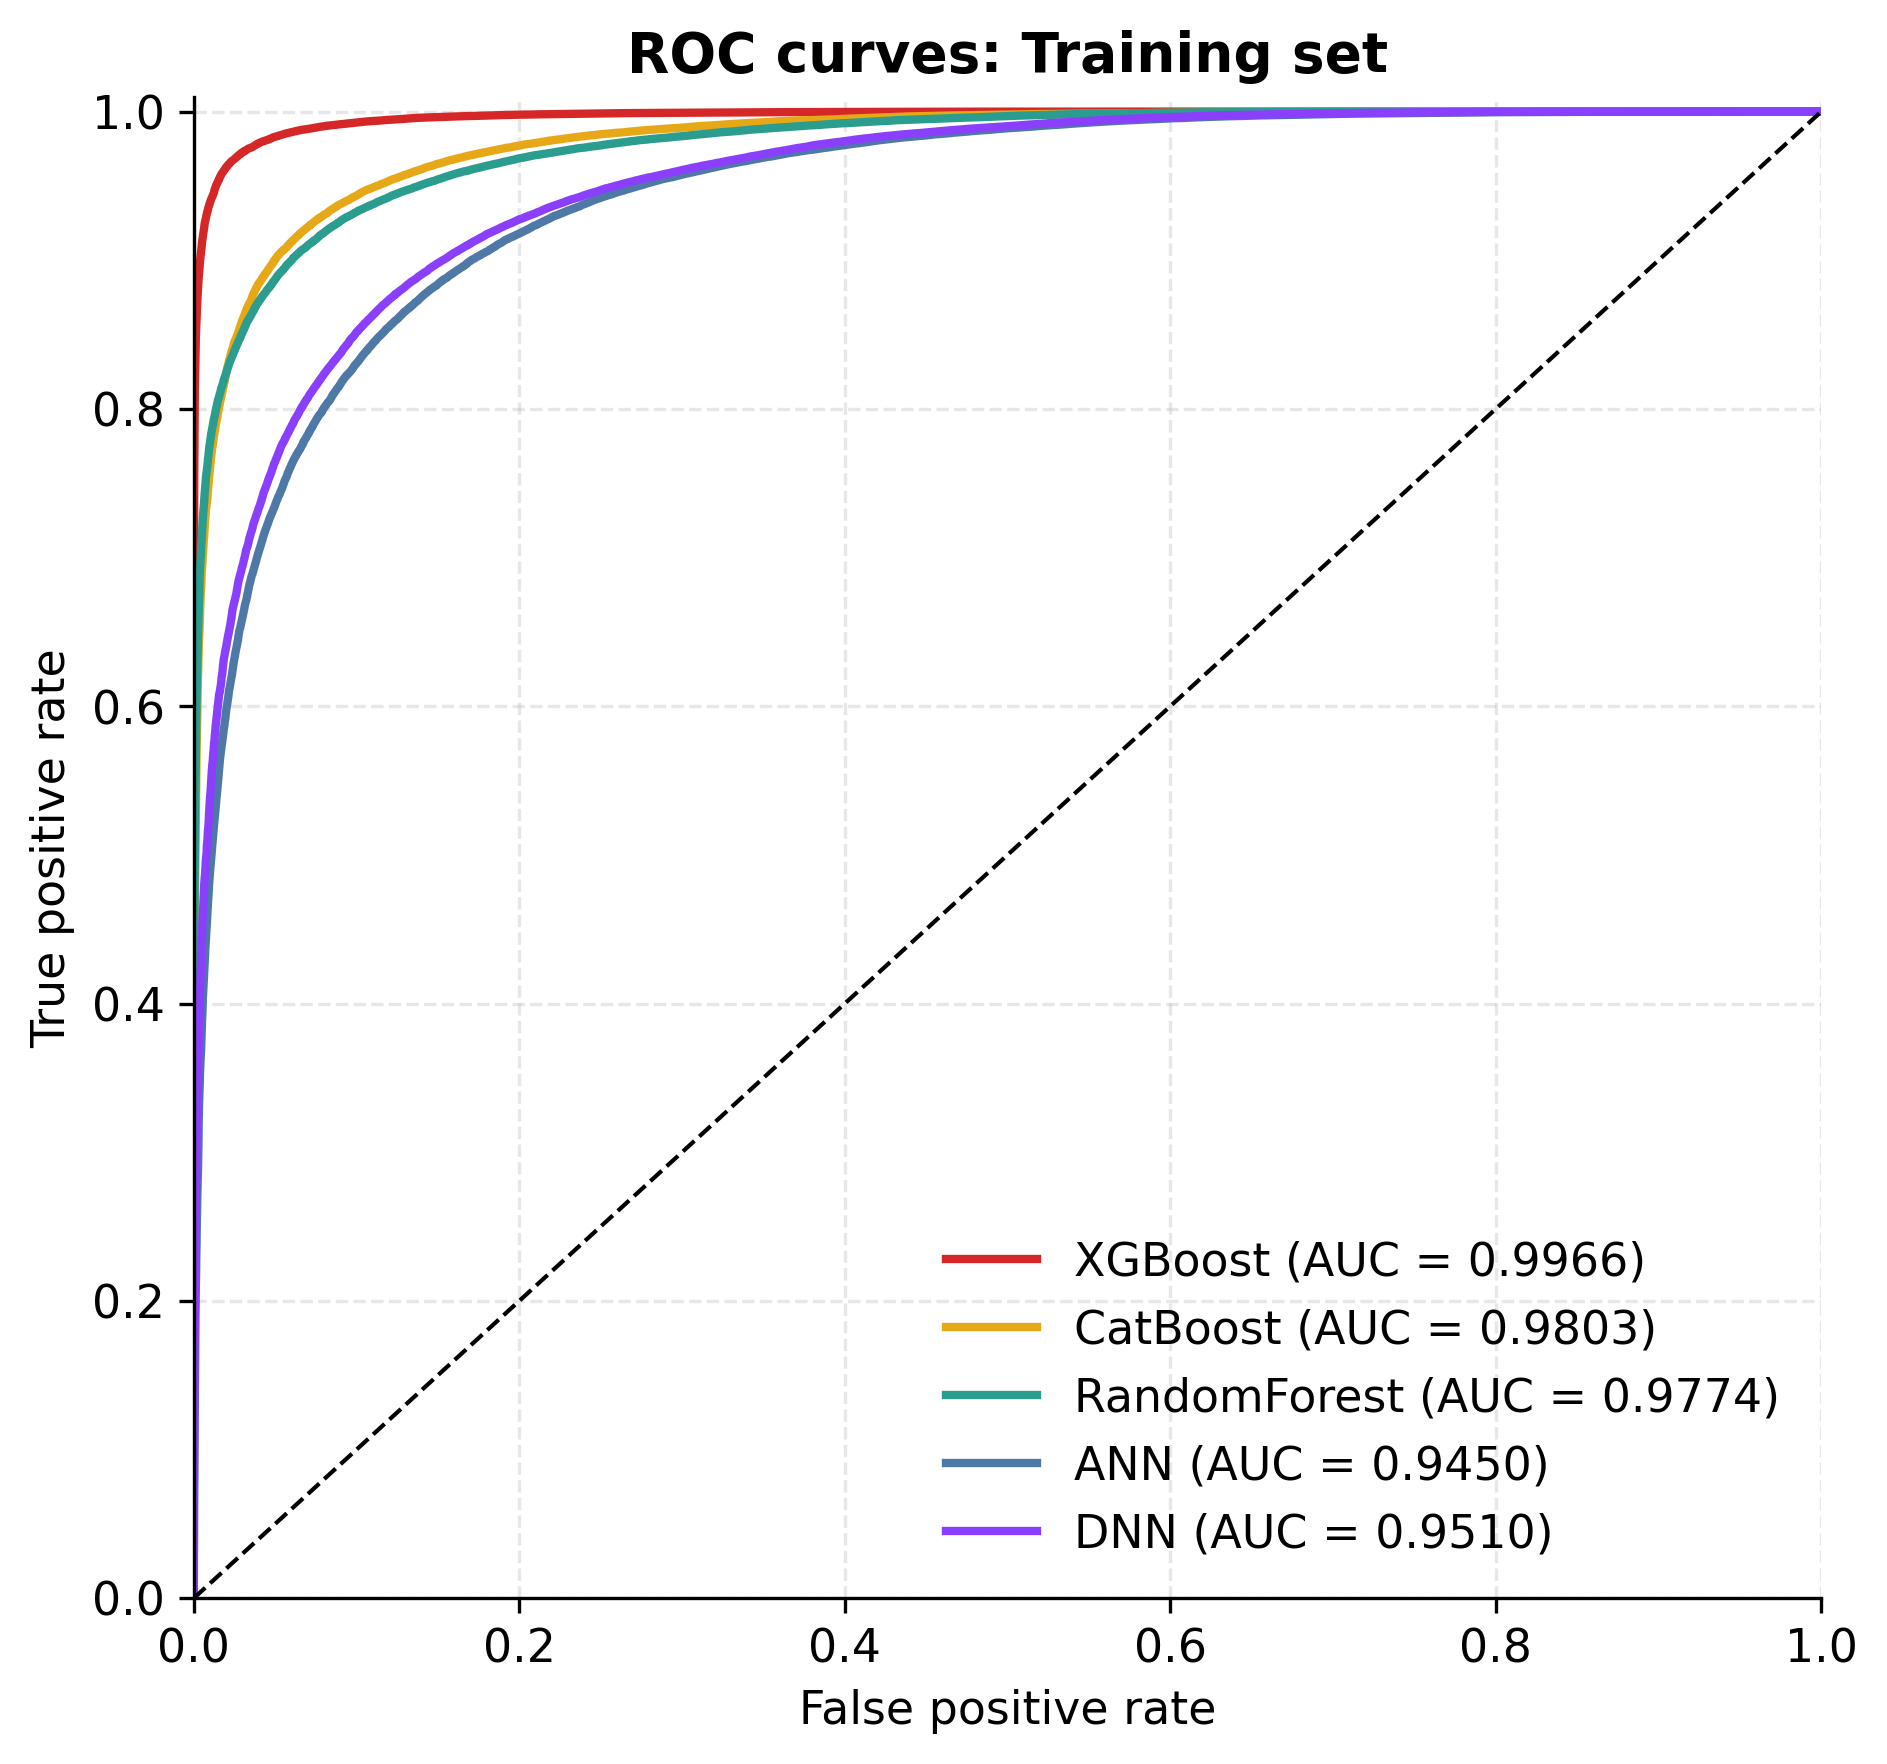
\includegraphics[width=0.90\textwidth]{Figures_v2/Training__ROC.png}
    \caption{ROC curves for all five models on the training set (200,000-pixel random subsample of the 70\% training split). AUC values are reported in parentheses. Training AUC is close to the test AUC (Figure~\ref{fig:roc_val}) for every model.}
    \label{fig:roc_train}
\end{figure}

\begin{figure}[H]
    \centering
    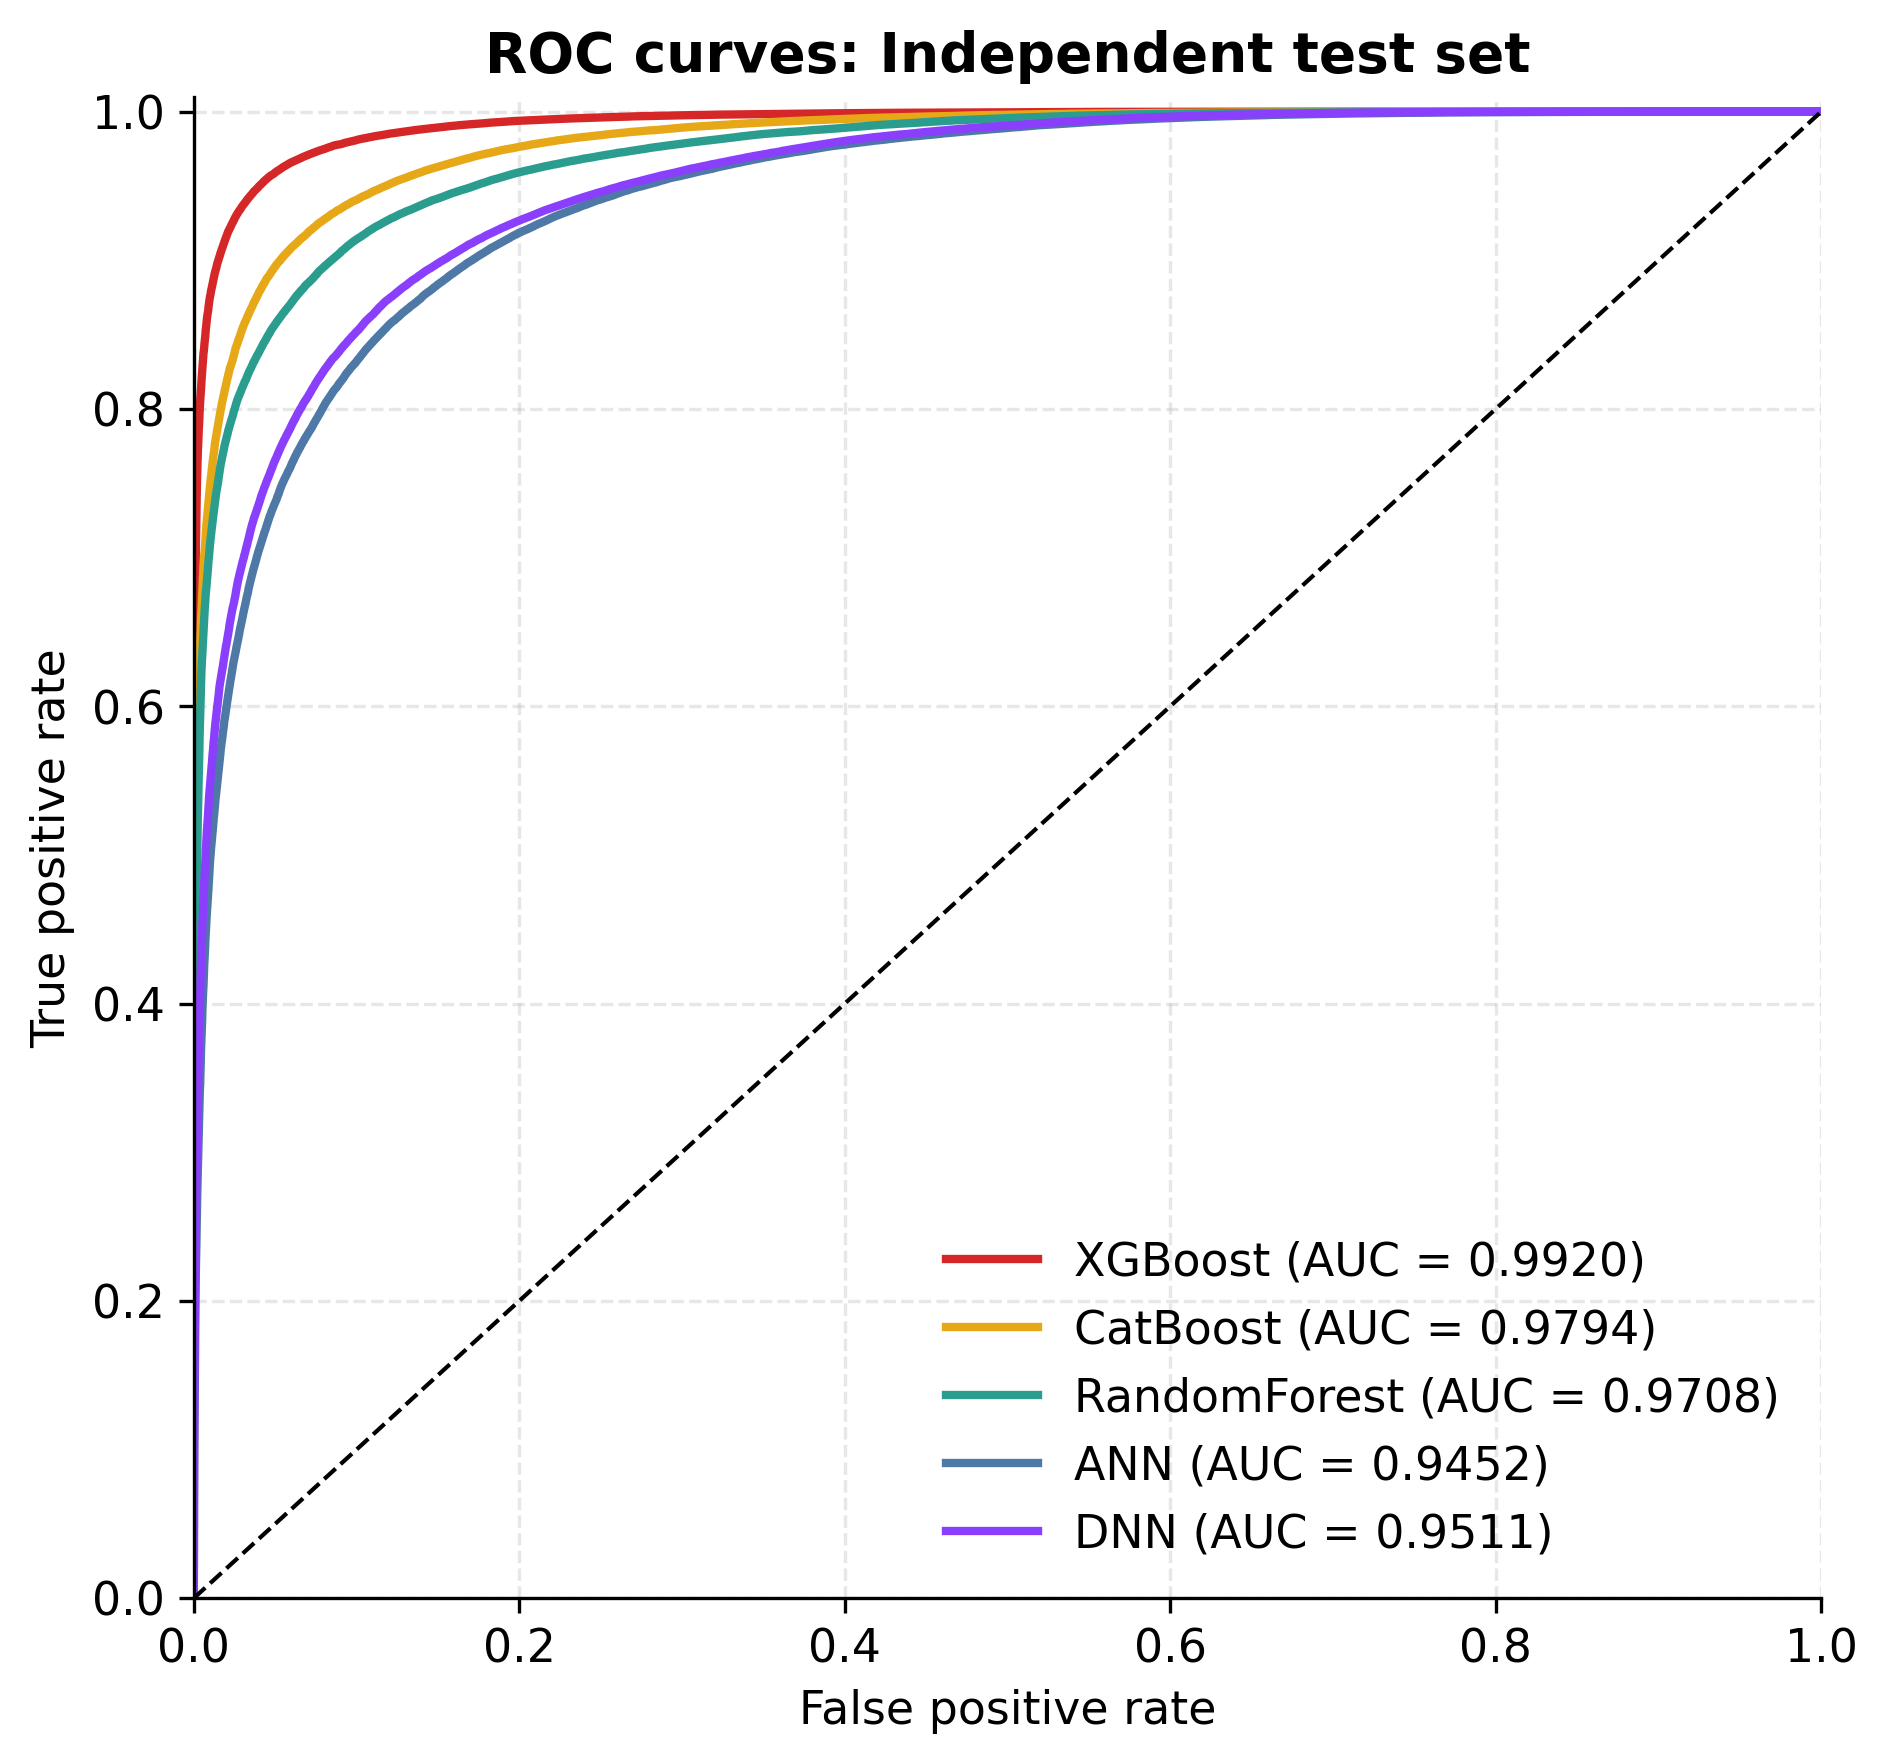
\includegraphics[width=0.90\textwidth]{Figures_v2/Validation_ROC.png}
    \caption{ROC curves for all five models on the independent test set (20\% of district pixels, never used for training, early stopping, or threshold selection). AUC values are reported in parentheses. XGBoost (AUC = 0.9920), CatBoost (0.9794), and RF (0.9708) lie above DNN (0.9511) and ANN (0.9452) across most of the FPR range.}
    \label{fig:roc_val}
\end{figure}

\subsection{Threshold Method Comparison: Max-CSI vs.\ Youden's Index}

Max-CSI gave a higher test CSI than Youden's Index for all five models (Table~\ref{tab:threshold}), but the gains are small: from +0.0022 (XGBoost) to +0.0083 (ANN), with a mean of +0.0048. Max-CSI thresholds were consistently \textit{lower} than Youden's thresholds (0.429--0.494 against 0.527--0.560; Figure~\ref{fig:maxcsi}c): with flood pixels forming 56\% of the district, maximising the CSI favours sensitivity (Max-CSI sensitivity exceeds Youden sensitivity by 0.015--0.046), at the cost of some specificity. The fixed 0.5 cut-off performs almost as well as Max-CSI here (CSI within 0.0035 for every model), because the classes are nearly balanced and the probabilities are reasonably calibrated; the value of Max-CSI is that it selects a threshold for the operational objective explicitly instead of relying on these conditions.

\begin{table}[H]
\centering
\caption{Max-CSI and Youden's Index thresholds (chosen on the validation set) and the test-set CSI at each. $\Delta$CSI is the CSI gain of Max-CSI over Youden's Index.}
\label{tab:threshold}
\begin{adjustbox}{max width=\linewidth}
\begin{tabular}{lcccccc}
\toprule
\multirow{2}{*}{\textbf{Model}} & \multicolumn{2}{c}{\textbf{Max-CSI}} & \multicolumn{2}{c}{\textbf{Youden's Index}} & \multirow{2}{*}{\textbf{$\Delta$CSI}} \\
\cmidrule(lr){2-3}\cmidrule(lr){4-5}
 & $\tau^*$ & CSI & $\tau^*$ & CSI & \\
\midrule
XGBoost       & 0.493 & 0.9229 & 0.551 & 0.9206 & +0.0022 \\
CatBoost      & 0.494 & 0.8731 & 0.560 & 0.8696 & +0.0035 \\
RandomForest  & 0.487 & 0.8483 & 0.527 & 0.8460 & +0.0023 \\
DNN           & 0.446 & 0.8041 & 0.553 & 0.7966 & +0.0075 \\
ANN           & 0.429 & 0.7946 & 0.544 & 0.7862 & +0.0083 \\
\bottomrule
\end{tabular}
\end{adjustbox}
\end{table}

\begin{figure}[H]
    \centering
    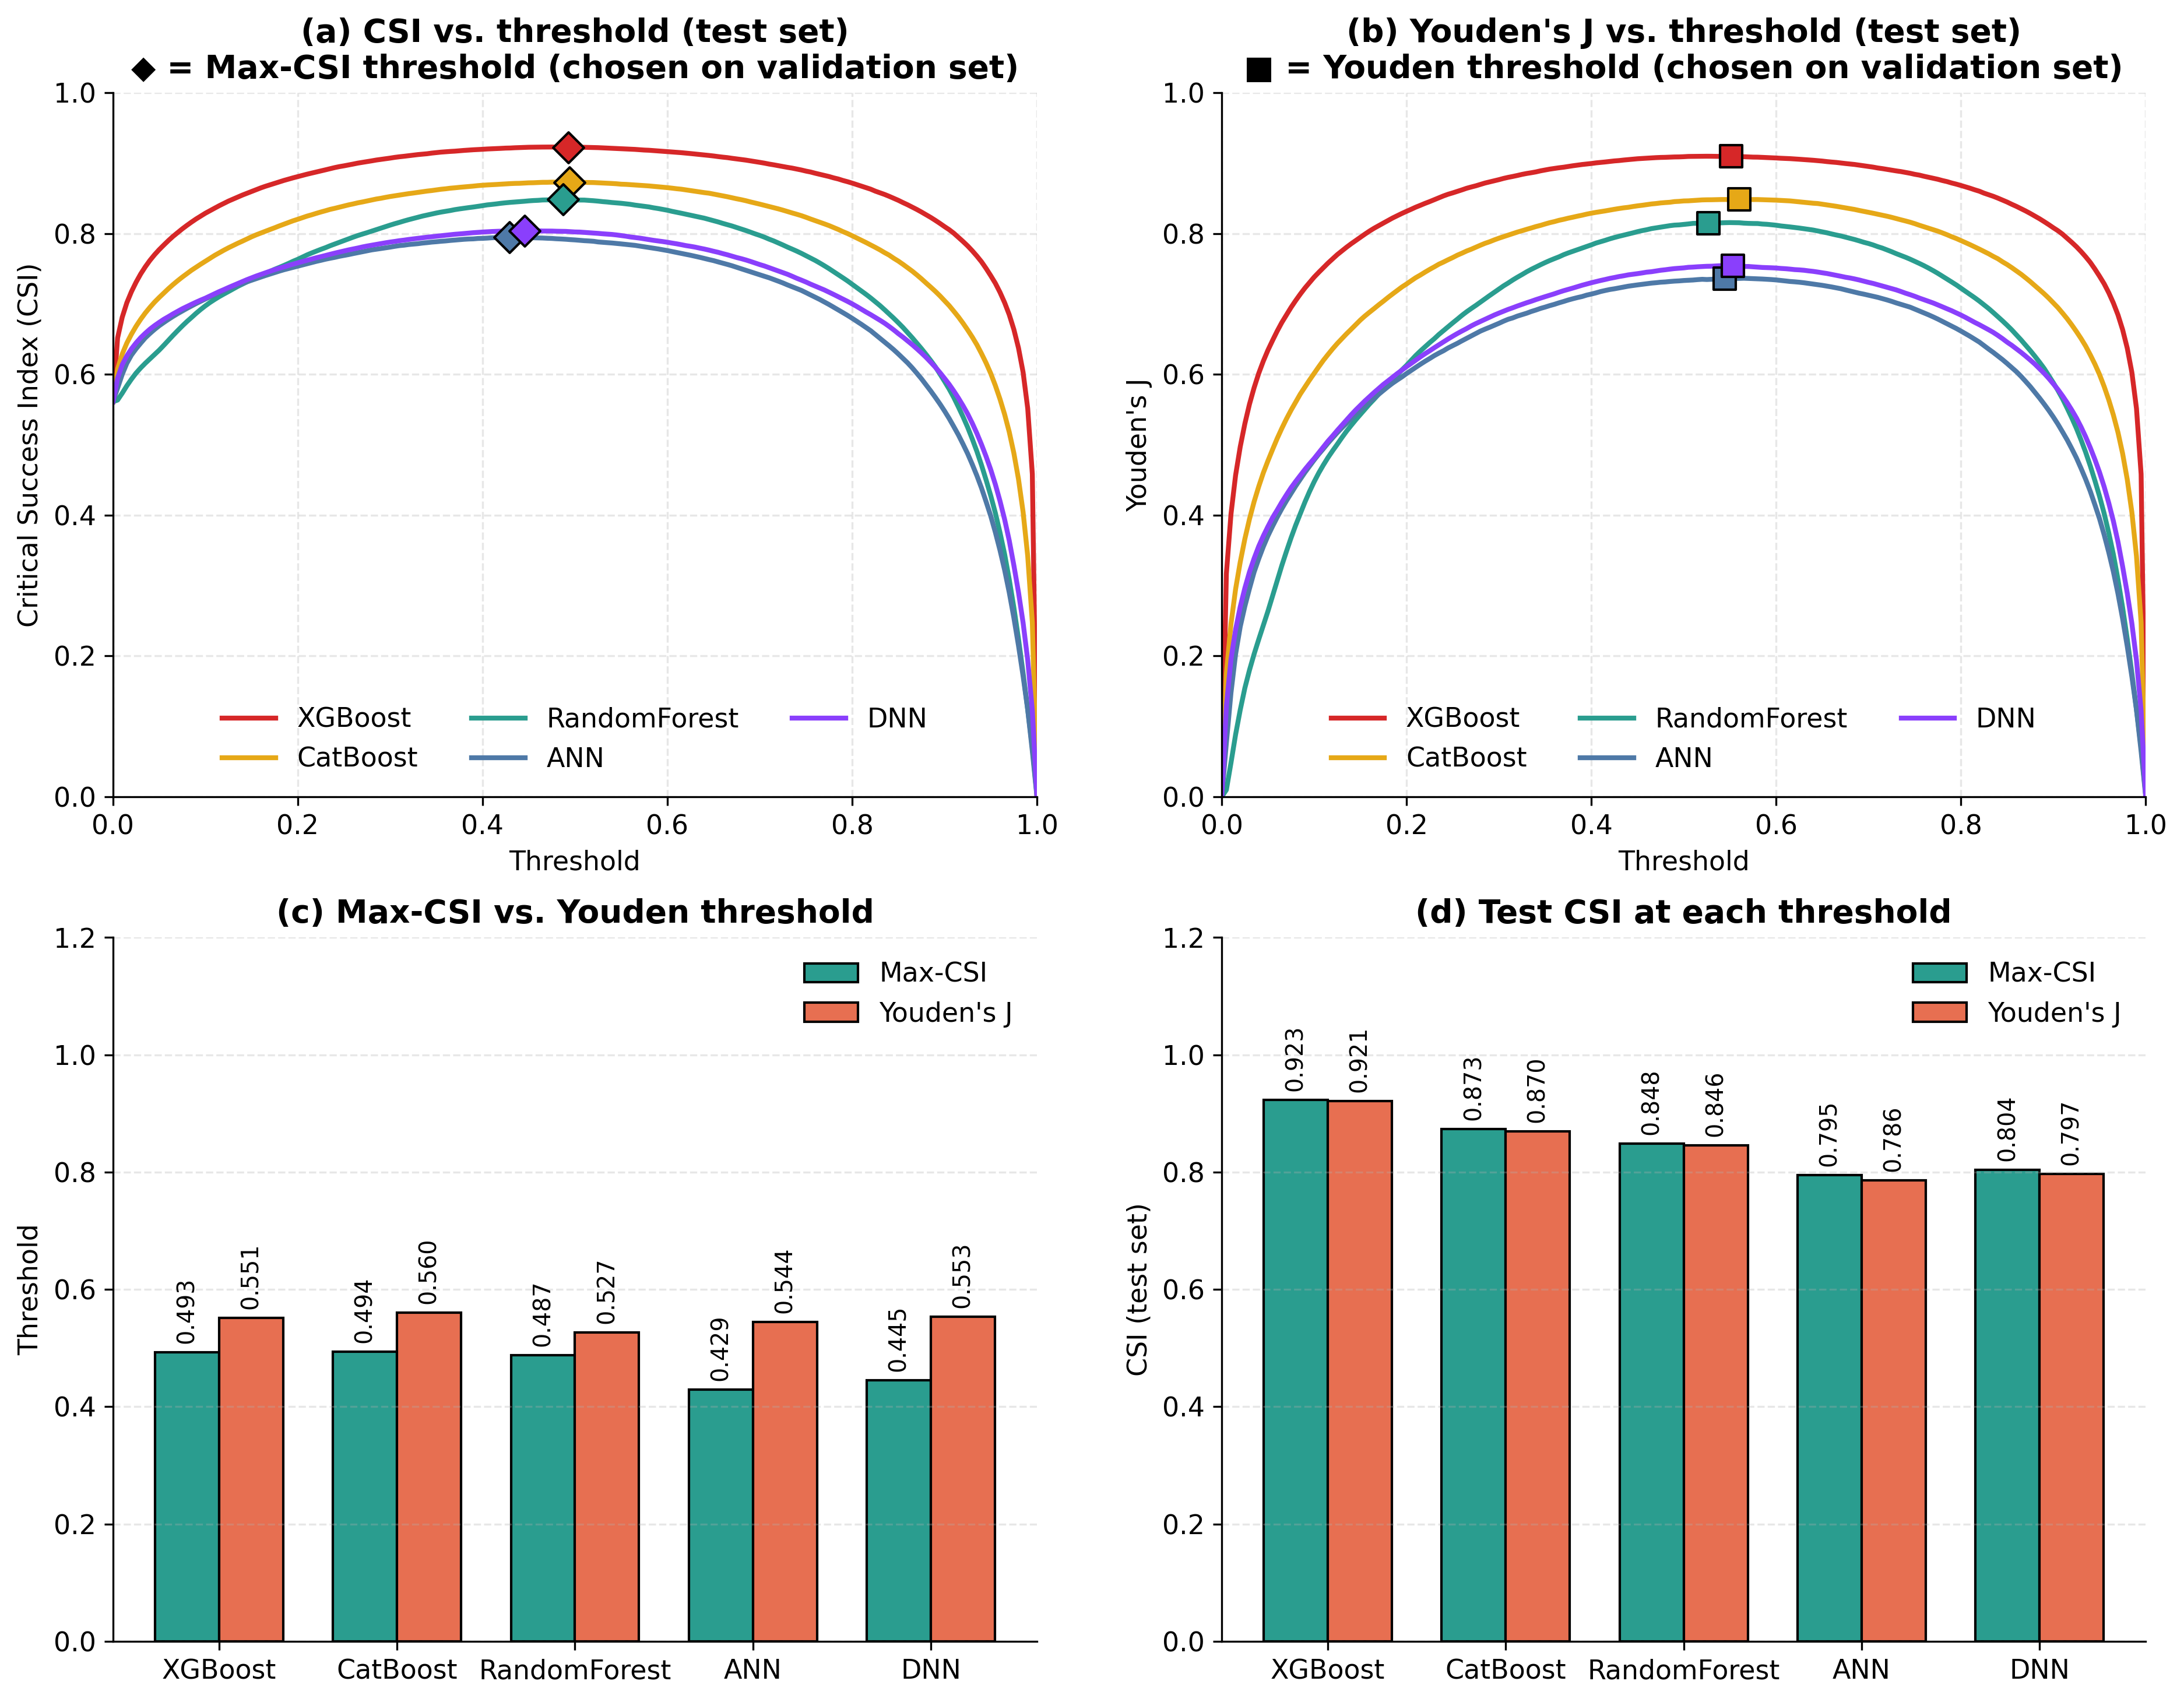
\includegraphics[width=\textwidth]{Figures_v2/Fig_MaxCSI_Threshold_Analysis.png}
    \caption{Threshold analysis for all five models on the independent test set. (a) CSI vs.\ probability threshold; diamonds mark the Max-CSI threshold ($\tau^*$) chosen on the validation set. (b) Youden's J vs.\ threshold; squares mark the Youden threshold chosen on the validation set. (c) Max-CSI and Youden thresholds. (d) Test CSI at the Max-CSI threshold (teal) and the Youden threshold (red). The CSI curves are flat near their maxima, so the gain from Max-CSI is small but consistent.}
    \label{fig:maxcsi}
\end{figure}

\subsection{SHAP-Based Conditioning Factor Importance}
\label{sec:shap}

To identify the dominant drivers of flood susceptibility and quantify their individual contributions to model predictions, SHapley Additive exPlanations (SHAP) values were computed for all five trained models \citep{lundberg2017, lundberg2020}.  SHAP assigns each conditioning factor a contribution $\phi_j$ for each pixel prediction, satisfying the efficiency, symmetry, linearity, and dummy Shapley axioms \citep{shapley1953}:
\begin{equation}
  f(\mathbf{x}) = \phi_0 + \sum_{j=1}^{p} \phi_j
  \label{eq:shap}
\end{equation}
where $f(\mathbf{x})$ is the model output and $\phi_0$ is the baseline expected output.  Mean absolute SHAP values $\bar{|\phi_j|} = N^{-1}\sum_i |\phi_{ij}|$ over the balanced sample of $N = 5{,}000$ test pixels (Section~\ref{sec:shap_method}) measure each CgF's average contribution to the predictions.

\subsubsection{Cross-Model SHAP Rankings}

Table~\ref{tab:shap} presents the normalised mean absolute SHAP scores under XGBoost, and Table~\ref{tab:shap_allmodels} and Figure~\ref{fig:shap_heatmap} compare all five models. Per-model beeswarm plots are shown in Figure~\ref{fig:shap_beeswarm_xgb} and Figures~\ref{fig:shap_beeswarm_cat}--\ref{fig:shap_beeswarm_dnn}.

\begin{table}[H]
\centering
\caption{Normalised mean $|\text{SHAP}|$ scores for the fourteen conditioning factors under XGBoost (TreeSHAP; $N = 5{,}000$ balanced test pixels). Scores are min--max normalised to $[0,1]$. The cross-model rank column gives the range of ranks over all five models (Table~\ref{tab:shap_allmodels}).}
\label{tab:shap}
\begin{adjustbox}{max width=\linewidth}
\begin{tabular}{clccc}
\toprule
\textbf{Rank} & \textbf{Conditioning Factor} & \textbf{SHAP Score} & \textbf{Cross-model Rank} & \textbf{Physical Role} \\
\midrule
1  & Rainfall           & 1.000 & 1--4  & Monsoon precipitation (smooth regional field) \\
2  & Geomorphology      & 0.993 & 1--2  & Landform unit: \textit{chaur}, levee, active channel \\
3  & Soil Type          & 0.816 & 1--3  & Infiltration capacity and runoff generation \\
4  & Elevation          & 0.594 & 3--4  & Gravitational drainage gradient \\
5  & Dist.\ to Roads    & 0.420 & 5--8  & Road embankment drainage obstruction \\
6  & Stream Density     & 0.371 & 6--8  & Drainage network concentration \\
7  & Dist.\ to Stream   & 0.362 & 6--7  & Proximity to bank overflow source \\
8  & LULC               & 0.300 & 5--8  & Surface imperviousness and roughness \\
9  & Stream Power Index & 0.129 & 9--10 & Erosive energy proxy \\
10 & Lithology          & 0.110 & 9--10 & Substrate permeability \\
11 & TWI                & 0.065 & 11    & Soil saturation propensity \\
12 & Slope              & 0.028 & 12    & Local gradient \\
13 & Aspect             & 0.024 & 13    & Directional moisture exposure \\
14 & Curvature          & 0.000 & 14    & Concavity index \\
\bottomrule
\end{tabular}
\end{adjustbox}
\end{table}

\subsubsection{Dominant Predictors: Rainfall, Geomorphology, Soil, and Elevation}

The same four factors --- Rainfall, Geomorphology, Soil, and Elevation --- occupy ranks 1--4 in all five models; only their order differs. XGBoost ranks Rainfall first (1.000) with Geomorphology almost level (0.993); CatBoost ranks Geomorphology first; RF, ANN, and DNN rank Soil first.

\textbf{Geomorphology} ranks first or second in every model. In Khagaria's multi-river alluvial system, geomorphological unit type directly encodes inundation exposure: \textit{chaur} depressions (abandoned meander ox-bow basins) flood first and drain last; active channel belts and Kosi sand bars are intermittently inundated; natural levees adjacent to the main channels resist all but catastrophic events; and older alluvial terraces (\textit{diara} land) are inundated only during decadal-scale events. This process-level separation is information that no single topometric index carries. In the beeswarm plot (Figure~\ref{fig:shap_beeswarm_xgb}), the most extensive unit (class code 1, 60\% of the district) receives negative contributions and the remaining units positive ones.

\textbf{Soil Type} ranks first to third, reflecting the role of hydraulic conductivity in partitioning monsoon precipitation between infiltration and surface runoff. Fine-textured alluvial soils (clay-dominated Inceptisols and Entisols) in the \textit{chaur} depressions and older floodplain surfaces saturate quickly under sustained monsoon rain, after which most further precipitation becomes direct runoff. The soil layer is mapped at roughly 1 km resolution, and its straight unit boundaries are visible in the susceptibility maps (Section~\ref{sec:maps}).

\textbf{Rainfall} shows a monotonic positive relationship in the beeswarm plot: higher mean monsoon precipitation increases the predicted flood probability. Its importance should be interpreted with care. The rainfall layer is a smooth field interpolated from coarse gridded data (1,165--1,320 mm across the district), so it varies mainly with position; part of its SHAP importance is likely to reflect its use by the models as a regional location variable rather than a pixel-level physical trigger.

\textbf{Elevation} ranks third or fourth despite Khagaria's limited relief, because the pixel-level signal resolves the metre-scale transitions from \textit{chaur} depressions to levee ridges. Low elevation consistently increases the predicted flood probability (Figure~\ref{fig:shap_beeswarm_xgb}).

\subsubsection{Lower-Ranked Predictors and Physical Interpretation}

Distance to Roads, Stream Density, Distance to Stream, and LULC form a second tier (ranks 5--8 in every model). The relatively high rank of Distance to Roads reflects road embankments acting as hydraulic barriers that redirect and pond flood water in the low-gradient plain; LULC captures the water-retaining kharif paddy fields that dominate the district. SPI and Lithology follow (ranks 9--10). \textbf{TWI}, \textbf{Slope}, \textbf{Aspect}, and \textbf{Curvature} rank 11--14 in all five models: in near-flat terrain where slope estimates are dominated by DEM noise, these terrain derivatives carry little information beyond Elevation and Geomorphology.

\subsubsection{Cross-Model SHAP Consistency}

Figure~\ref{fig:shap_heatmap} shows the ranks across all five models. The rank agreement is high: the top four and the bottom four factors are identical sets in every model, and the middle tier differs only in order. ANN and DNN rankings are almost identical to each other and close to RF. This consistency supports a \textit{minimum viable feature set} (MVFS) of \{Geomorphology, Soil, Rainfall, Elevation\}, compilable from freely available datasets (Bhukosh, NBSS\&LUP, IMD/CHIRPS, SRTM), subject to the caveat on Rainfall above.

%% ── SHAP FIGURES ──────────────────────────────────────────────────────────

%% ── SHAP TABLE (replaces Fig_SHAP_All_Models bar chart) ──────────────────

\begin{table}[H]
\centering
\caption{Normalised mean $|\text{SHAP}|$ scores and feature importance ranks for all five models. Scores are min--max normalised to $[0,1]$ within each model. Rank 1 = most important.}
\label{tab:shap_allmodels}
\begin{adjustbox}{max width=\linewidth}
\begin{tabular}{l cc cc cc cc cc}
\toprule
\multirow{2}{*}{\textbf{Conditioning Factor}}
  & \multicolumn{2}{c}{\textbf{XGBoost}}
  & \multicolumn{2}{c}{\textbf{CatBoost}}
  & \multicolumn{2}{c}{\textbf{RandomForest}}
  & \multicolumn{2}{c}{\textbf{ANN}}
  & \multicolumn{2}{c}{\textbf{DNN}} \\
\cmidrule(lr){2-3}\cmidrule(lr){4-5}\cmidrule(lr){6-7}\cmidrule(lr){8-9}\cmidrule(lr){10-11}
  & Score & Rank & Score & Rank & Score & Rank & Score & Rank & Score & Rank \\
\midrule
Rainfall           & 1.000 & 1  & 0.805 & 3  & 0.724 & 3  & 0.546 & 4  & 0.628 & 4  \\
Geomorphology      & 0.993 & 2  & 1.000 & 1  & 0.982 & 2  & 0.975 & 2  & 0.985 & 2  \\
Soil Type          & 0.816 & 3  & 0.983 & 2  & 1.000 & 1  & 1.000 & 1  & 1.000 & 1  \\
Elevation          & 0.594 & 4  & 0.654 & 4  & 0.579 & 4  & 0.733 & 3  & 0.704 & 3  \\
Dist.\ to Roads    & 0.420 & 5  & 0.342 & 5  & 0.241 & 6  & 0.197 & 8  & 0.194 & 8  \\
Stream Density     & 0.371 & 6  & 0.280 & 8  & 0.162 & 8  & 0.199 & 7  & 0.208 & 7  \\
Dist.\ to Stream   & 0.362 & 7  & 0.341 & 6  & 0.241 & 7  & 0.216 & 6  & 0.209 & 6  \\
LULC               & 0.300 & 8  & 0.306 & 7  & 0.360 & 5  & 0.276 & 5  & 0.242 & 5  \\
Stream Power Index & 0.129 & 9  & 0.157 & 9  & 0.075 & 10 & 0.169 & 9  & 0.175 & 9  \\
Lithology          & 0.110 & 10 & 0.134 & 10 & 0.157 & 9  & 0.128 & 10 & 0.127 & 10 \\
TWI                & 0.065 & 11 & 0.059 & 11 & 0.037 & 11 & 0.053 & 11 & 0.058 & 11 \\
Slope              & 0.028 & 12 & 0.025 & 12 & 0.018 & 12 & 0.023 & 12 & 0.023 & 12 \\
Aspect             & 0.024 & 13 & 0.018 & 13 & 0.014 & 13 & 0.004 & 13 & 0.004 & 13 \\
Curvature          & 0.000 & 14 & 0.000 & 14 & 0.000 & 14 & 0.000 & 14 & 0.000 & 14 \\
\bottomrule
\multicolumn{11}{l}{\textit{Source: TreeSHAP (XGBoost, CatBoost, RF); \texttt{shap.GradientExplainer} (ANN, DNN).}} \\
\multicolumn{11}{l}{\textit{Sample: $N = 5{,}000$ balanced test pixels (2,500 flood; 2,500 non-flood). Scores min--max normalised per model.}} \\
\end{tabular}
\end{adjustbox}
\end{table}

\begin{figure}[H]
  \centering
  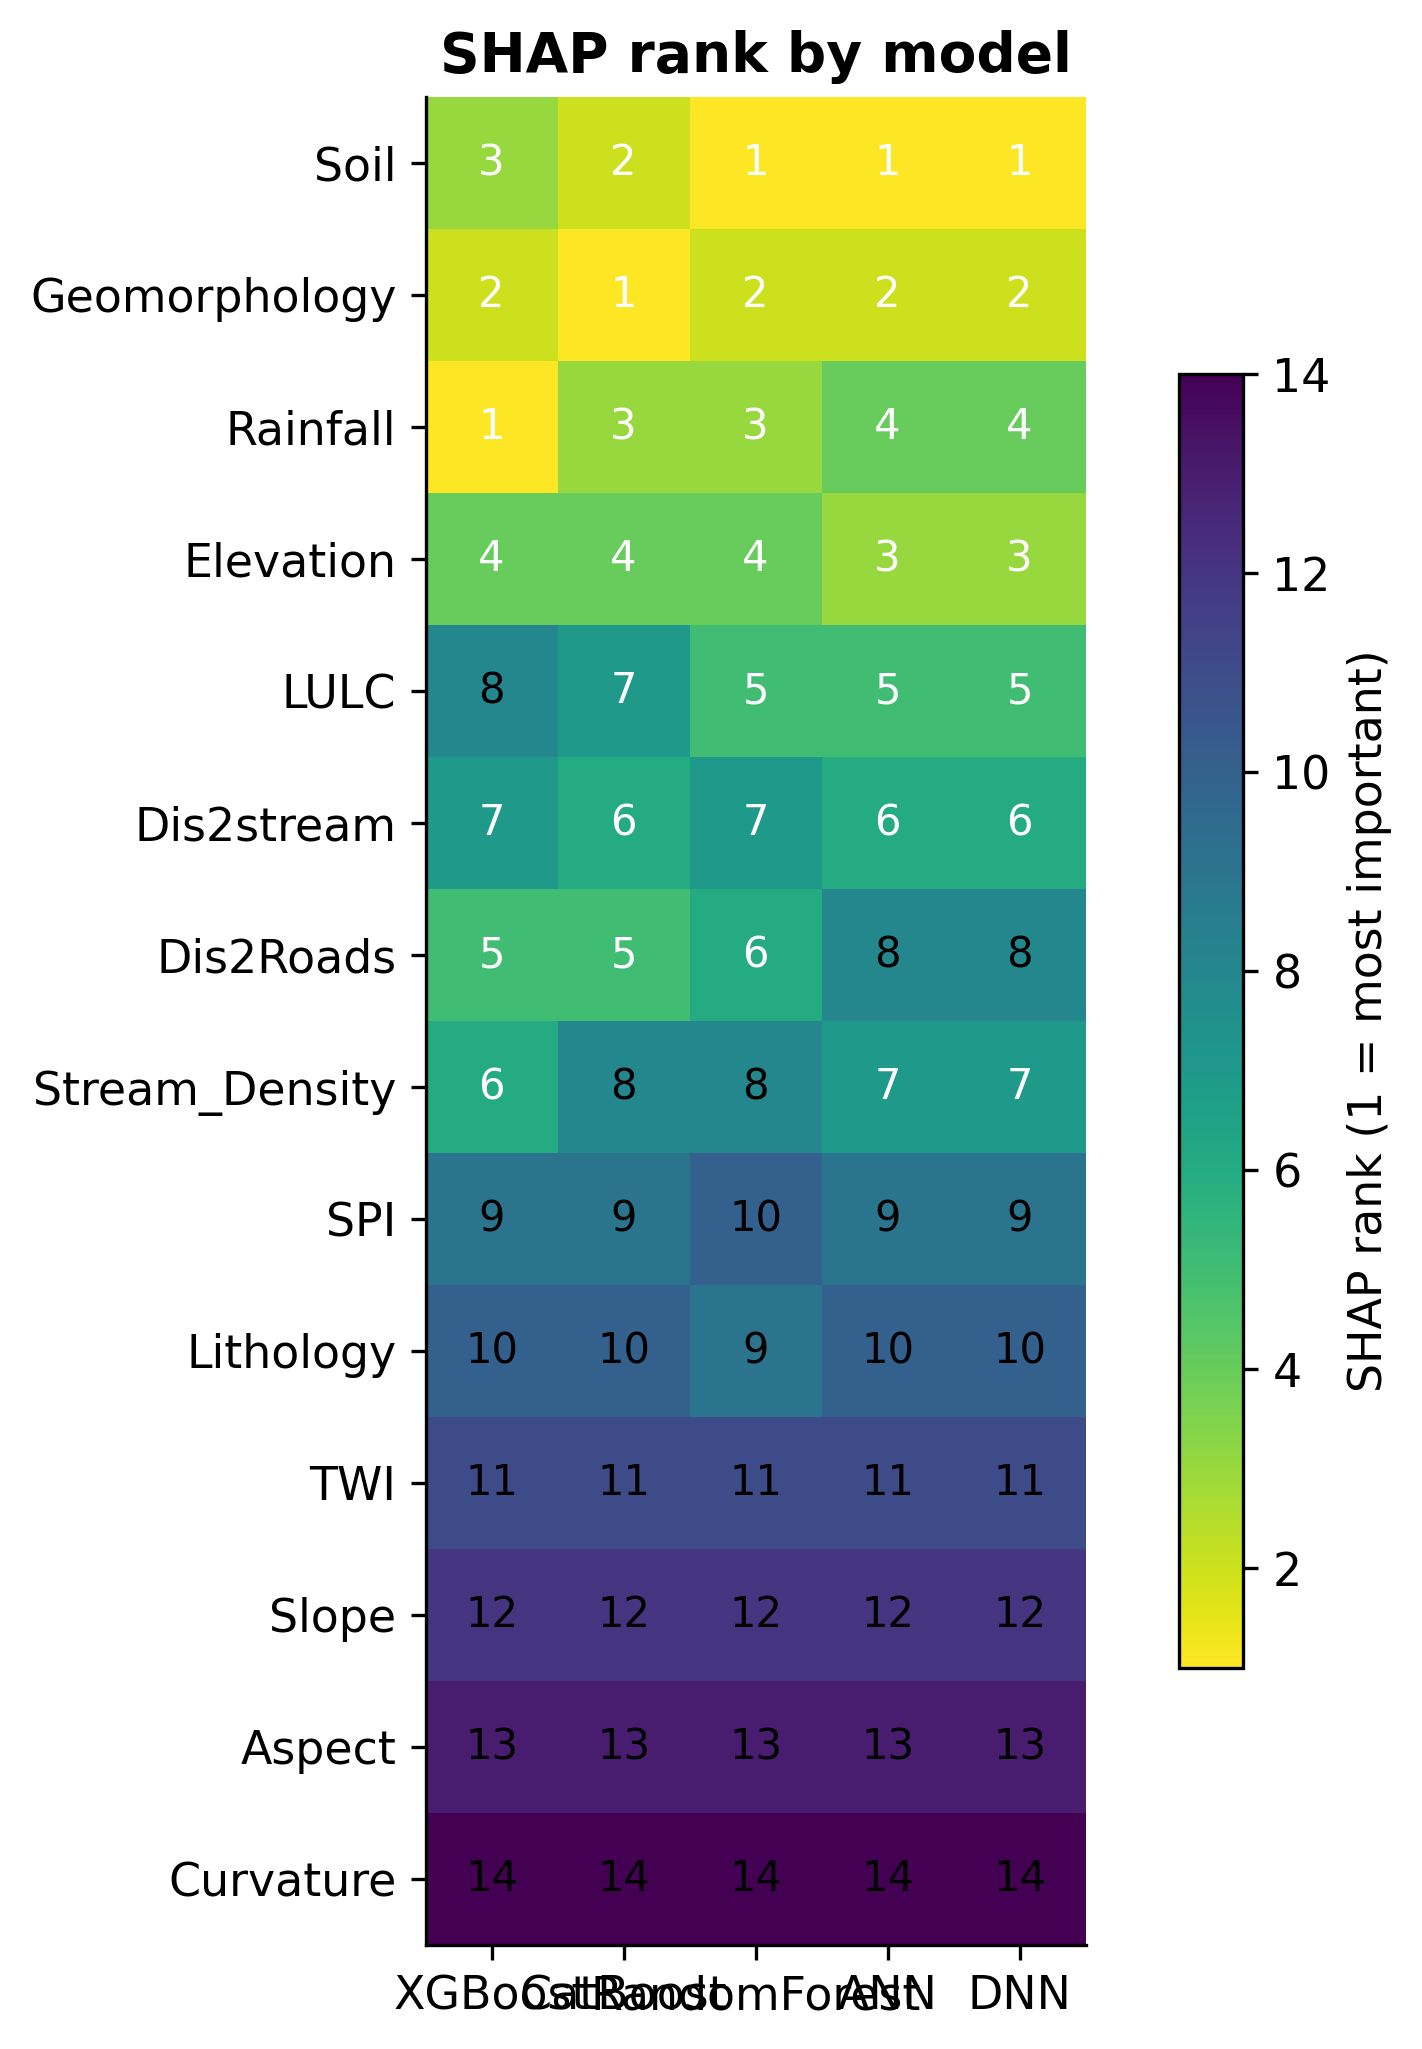
\includegraphics[width=0.75\textwidth]{Figures_v2/Fig_SHAP_Rank_Heatmap.png}
  \caption{Cross-model SHAP rank heatmap (rank 1 = most important). Rainfall, Geomorphology, Soil, and Elevation occupy ranks 1--4 in all five models, and TWI, Slope, Aspect, and Curvature ranks 11--14.}
  \label{fig:shap_heatmap}
\end{figure}

\begin{figure}[H]
  \centering
  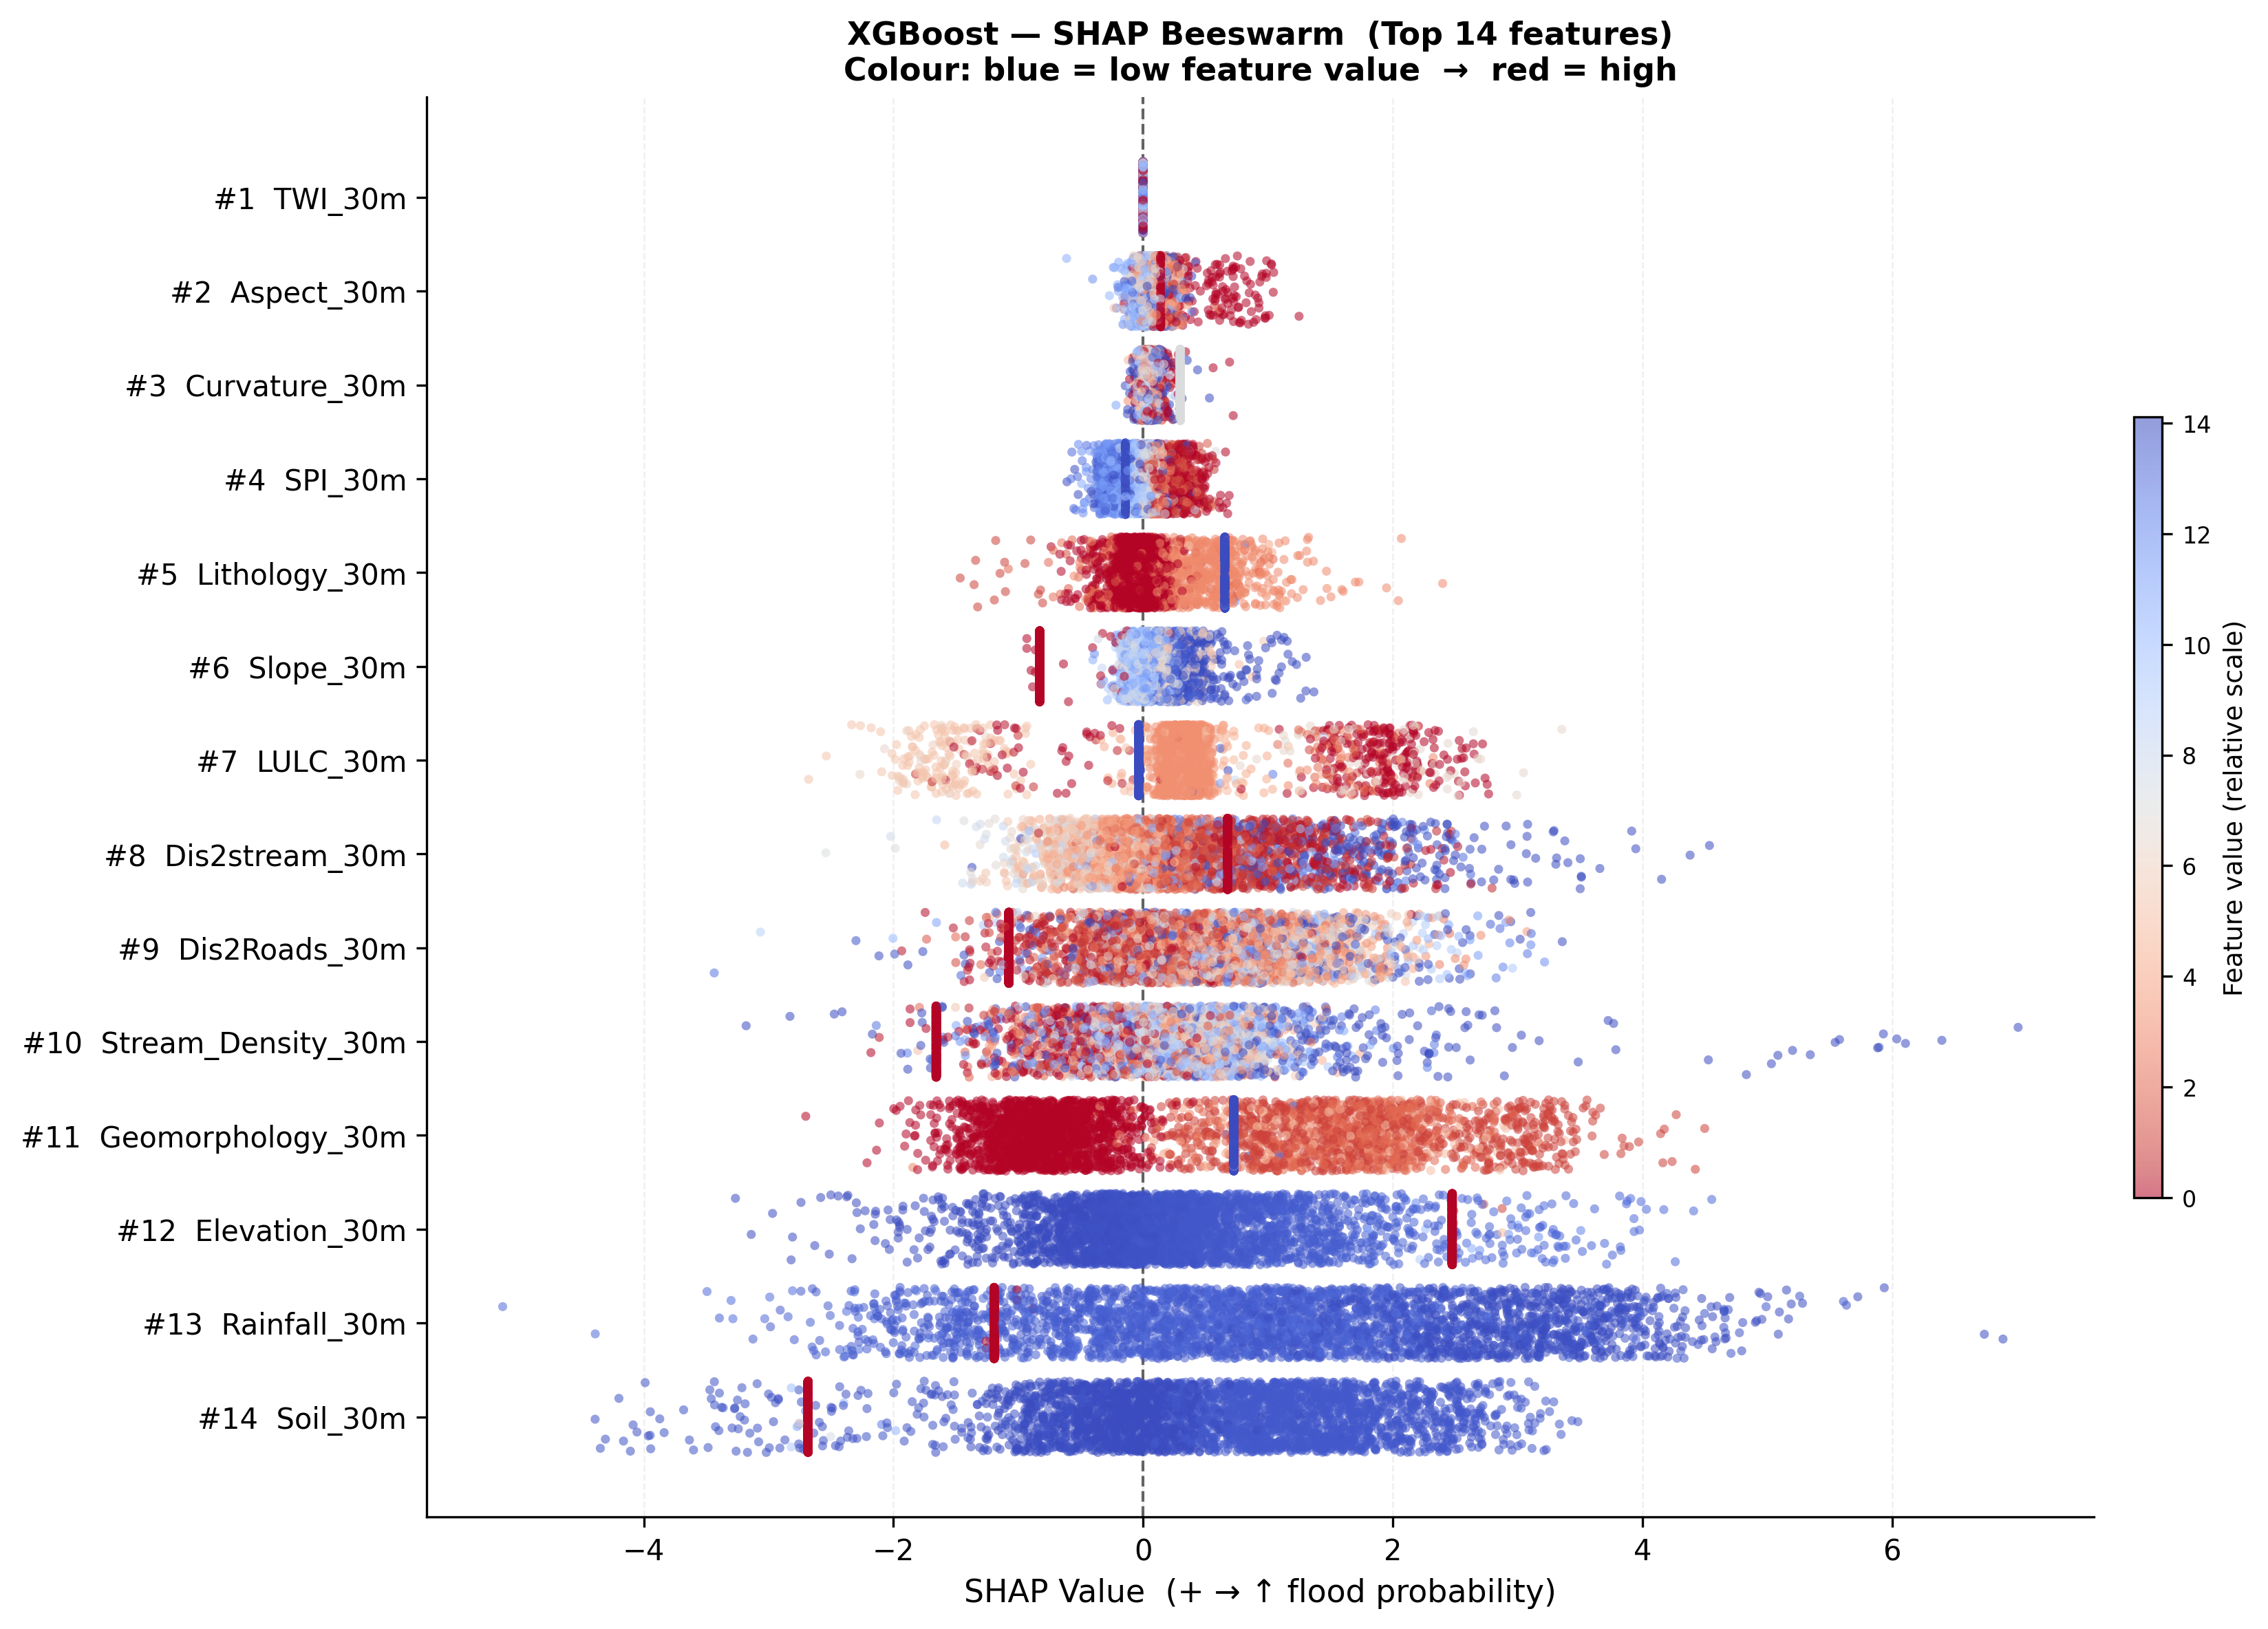
\includegraphics[width=\textwidth]{Figures/Fig_SHAP_Beeswarm_XGBoost.png}
  \caption{XGBoost SHAP beeswarm plot. Each point represents one of the 5,000 balanced test pixels; $x$-axis = SHAP value (positive = increased flood probability); colour = feature value (blue = low, red = high; for categorical factors the colour is the class code). Rainfall and Geomorphology have the widest spread. High rainfall and low elevation increase the predicted flood probability. Curvature, Aspect, and Slope have negligible spread.}
  \label{fig:shap_beeswarm_xgb}
\end{figure}

\subsection{Computational Efficiency}

All five models were trained on CPU (64 threads) in about two minutes in total for 1.14 million training pixels: RF in 11 s, XGBoost (1,000 rounds) in 37 s, CatBoost in 36 s, ANN in 16 s, and DNN in 27 s, including prediction of the validation and test sets. Training cost is therefore not a practical constraint for any of the models at district scale; the choice between them rests on accuracy.

\subsection{Flood Susceptibility and Hazard Maps}
\label{sec:maps}

\begin{figure}[H]
    \centering
    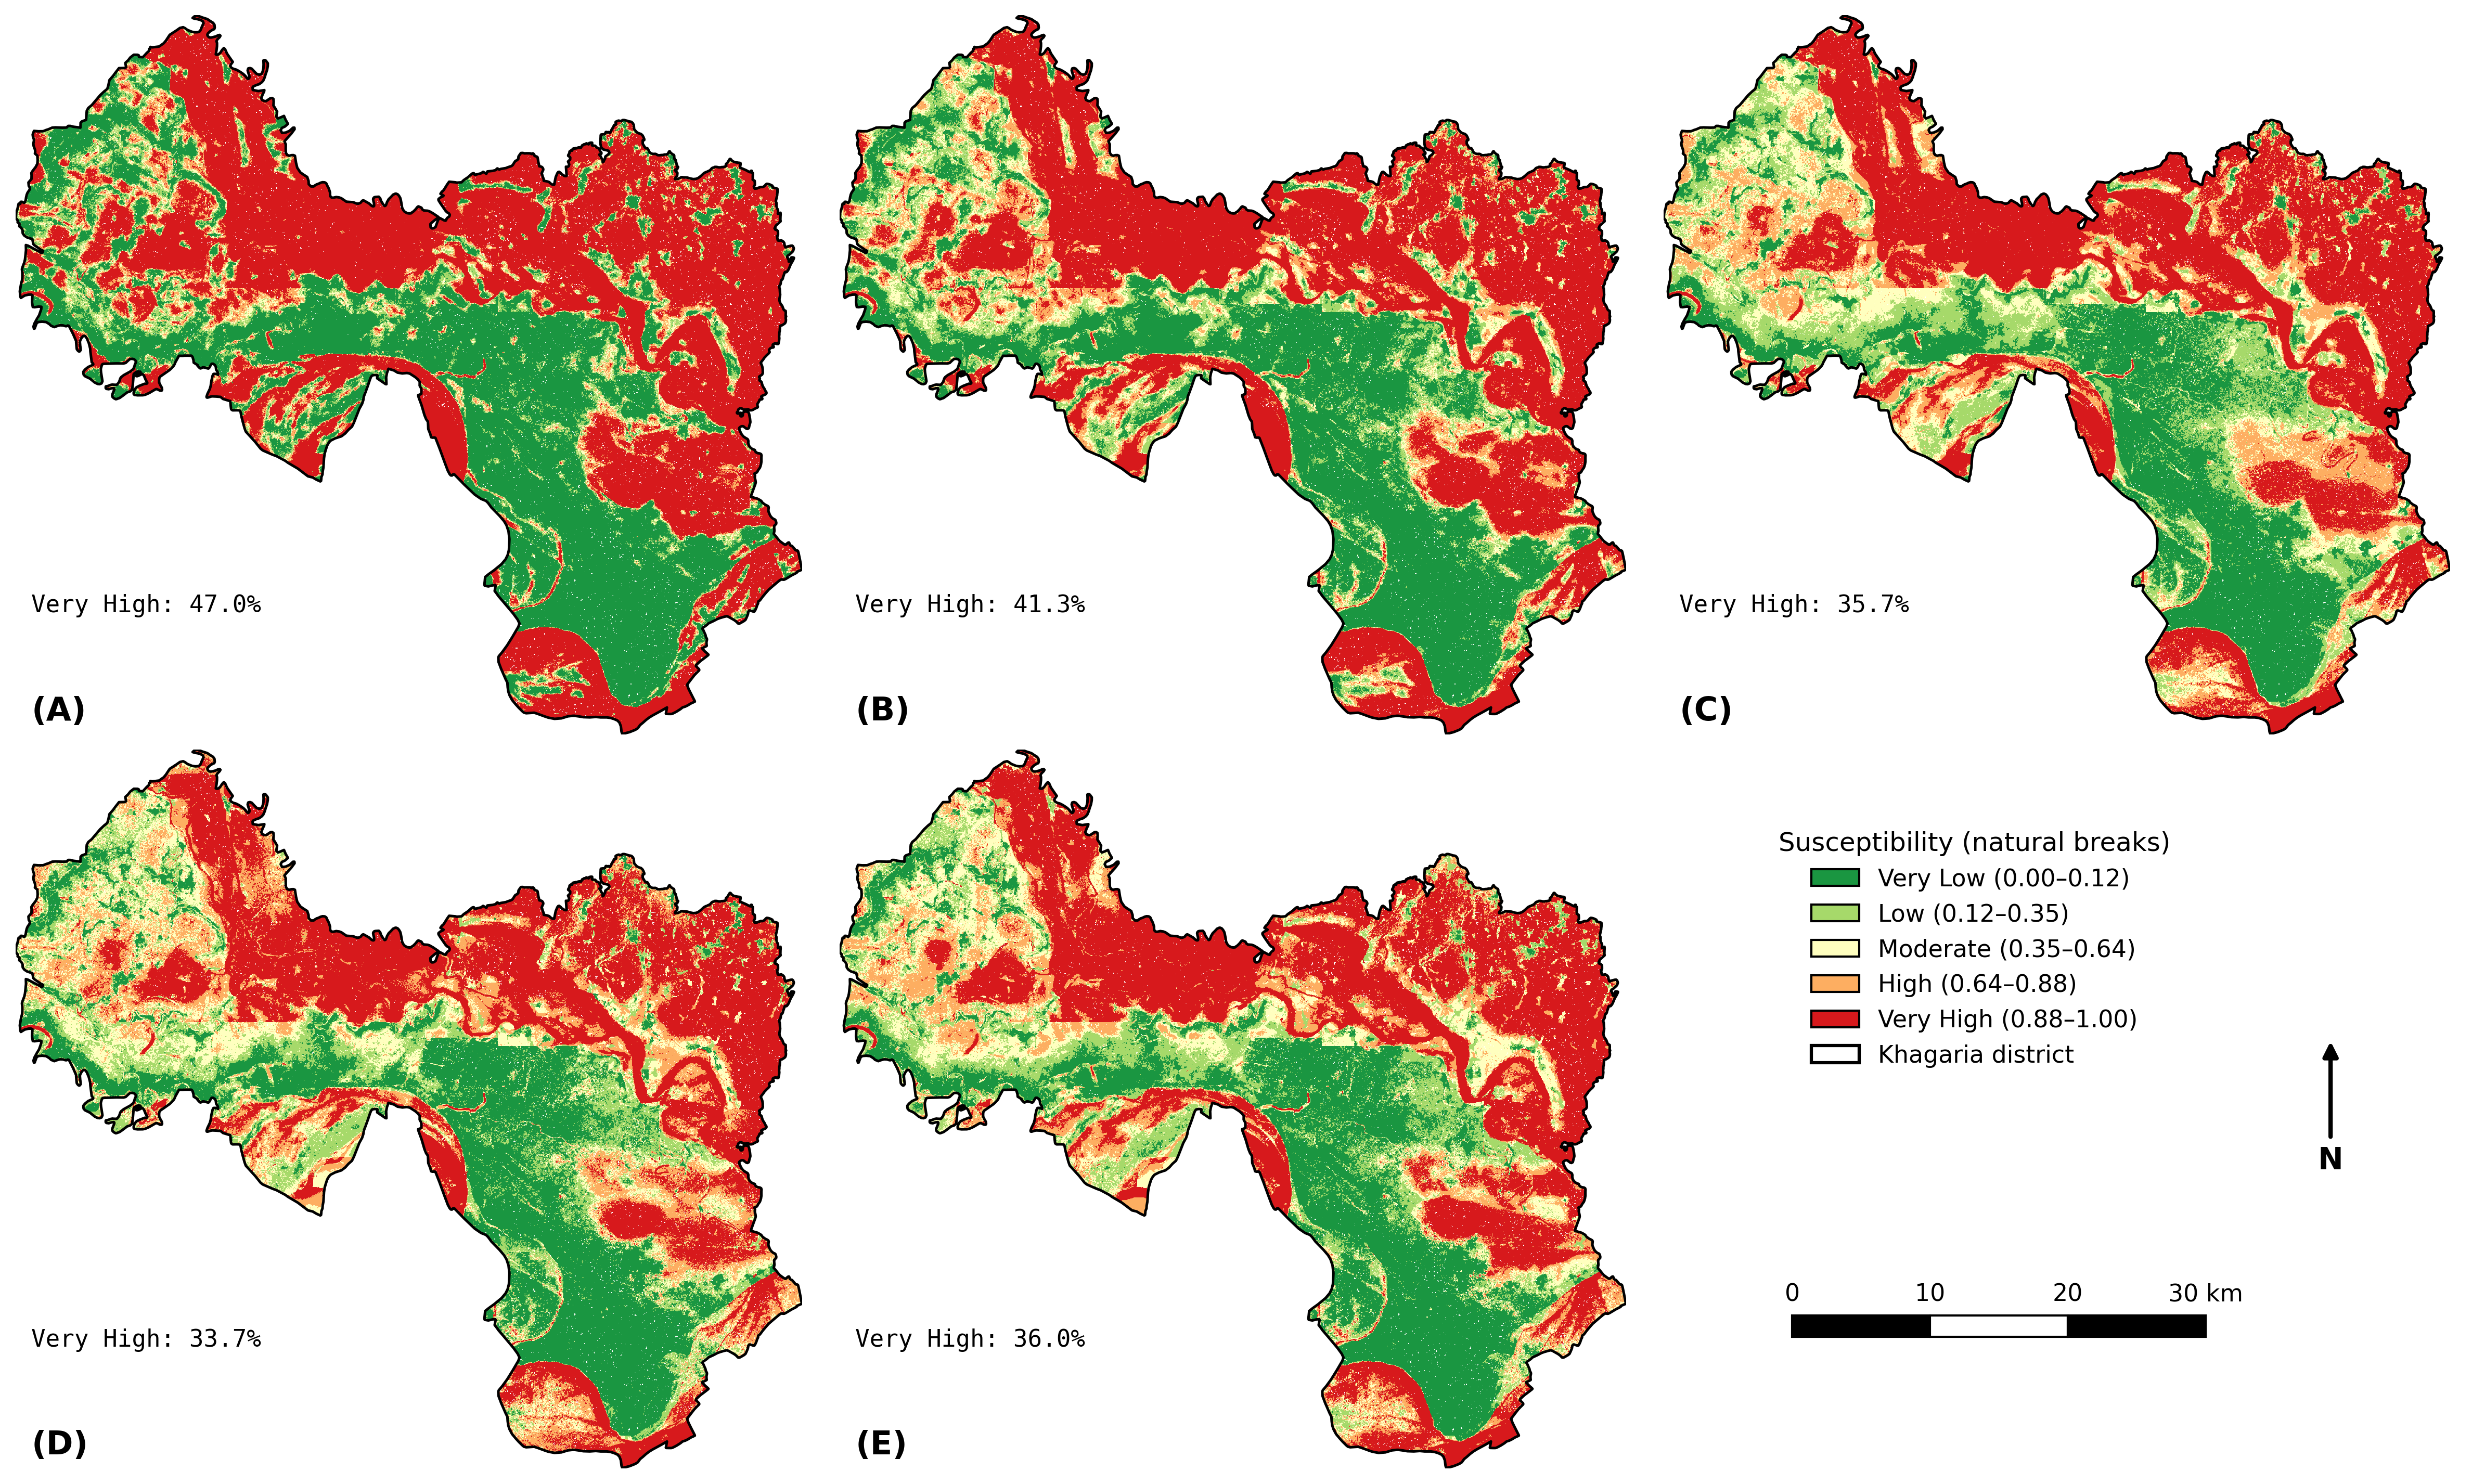
\includegraphics[width=\textwidth]{Figures_v2/Fig_Flood_Susceptibility_Maps.png}
    \caption{Flood susceptibility maps (FSMs) for Khagaria district from all five models, classified into five natural-break classes computed on the XGBoost map: Very Low (0.00--0.12), Low (0.12--0.35), Moderate (0.35--0.64), High (0.64--0.88), and Very High (0.88--1.00). (A) XGBoost; (B) CatBoost; (C) RandomForest; (D) ANN; (E) DNN. The share of the district in the Very High class is given in each panel. The straight east--west boundary across the centre of the district follows a unit boundary of the roughly 1 km soil map.}
    \label{fig:fsm}
\end{figure}

The five FSMs share the same large-scale pattern: Very High susceptibility in the Kosi meander belt across the north of the district, along the Burhi Gandak corridor, in the south-eastern backwater zone, and along the Ganga in the south, and Very Low susceptibility on the higher ground in the centre and south-centre. The \textit{chaur} depressions appear as isolated high-susceptibility patches. XGBoost (Figure~\ref{fig:fsm}A) produces the most polarised map, with most pixels in either the Very Low or the Very High class; CatBoost, RF, ANN, and DNN (Figures~\ref{fig:fsm}B--E) place progressively more area in the intermediate classes. A straight east--west line across the centre of the district in all five maps follows a unit boundary of the roughly 1 km soil map; it is an artefact of the input resolution, made visible because Soil is a top-three predictor.

\begin{figure}[H]
    \centering
    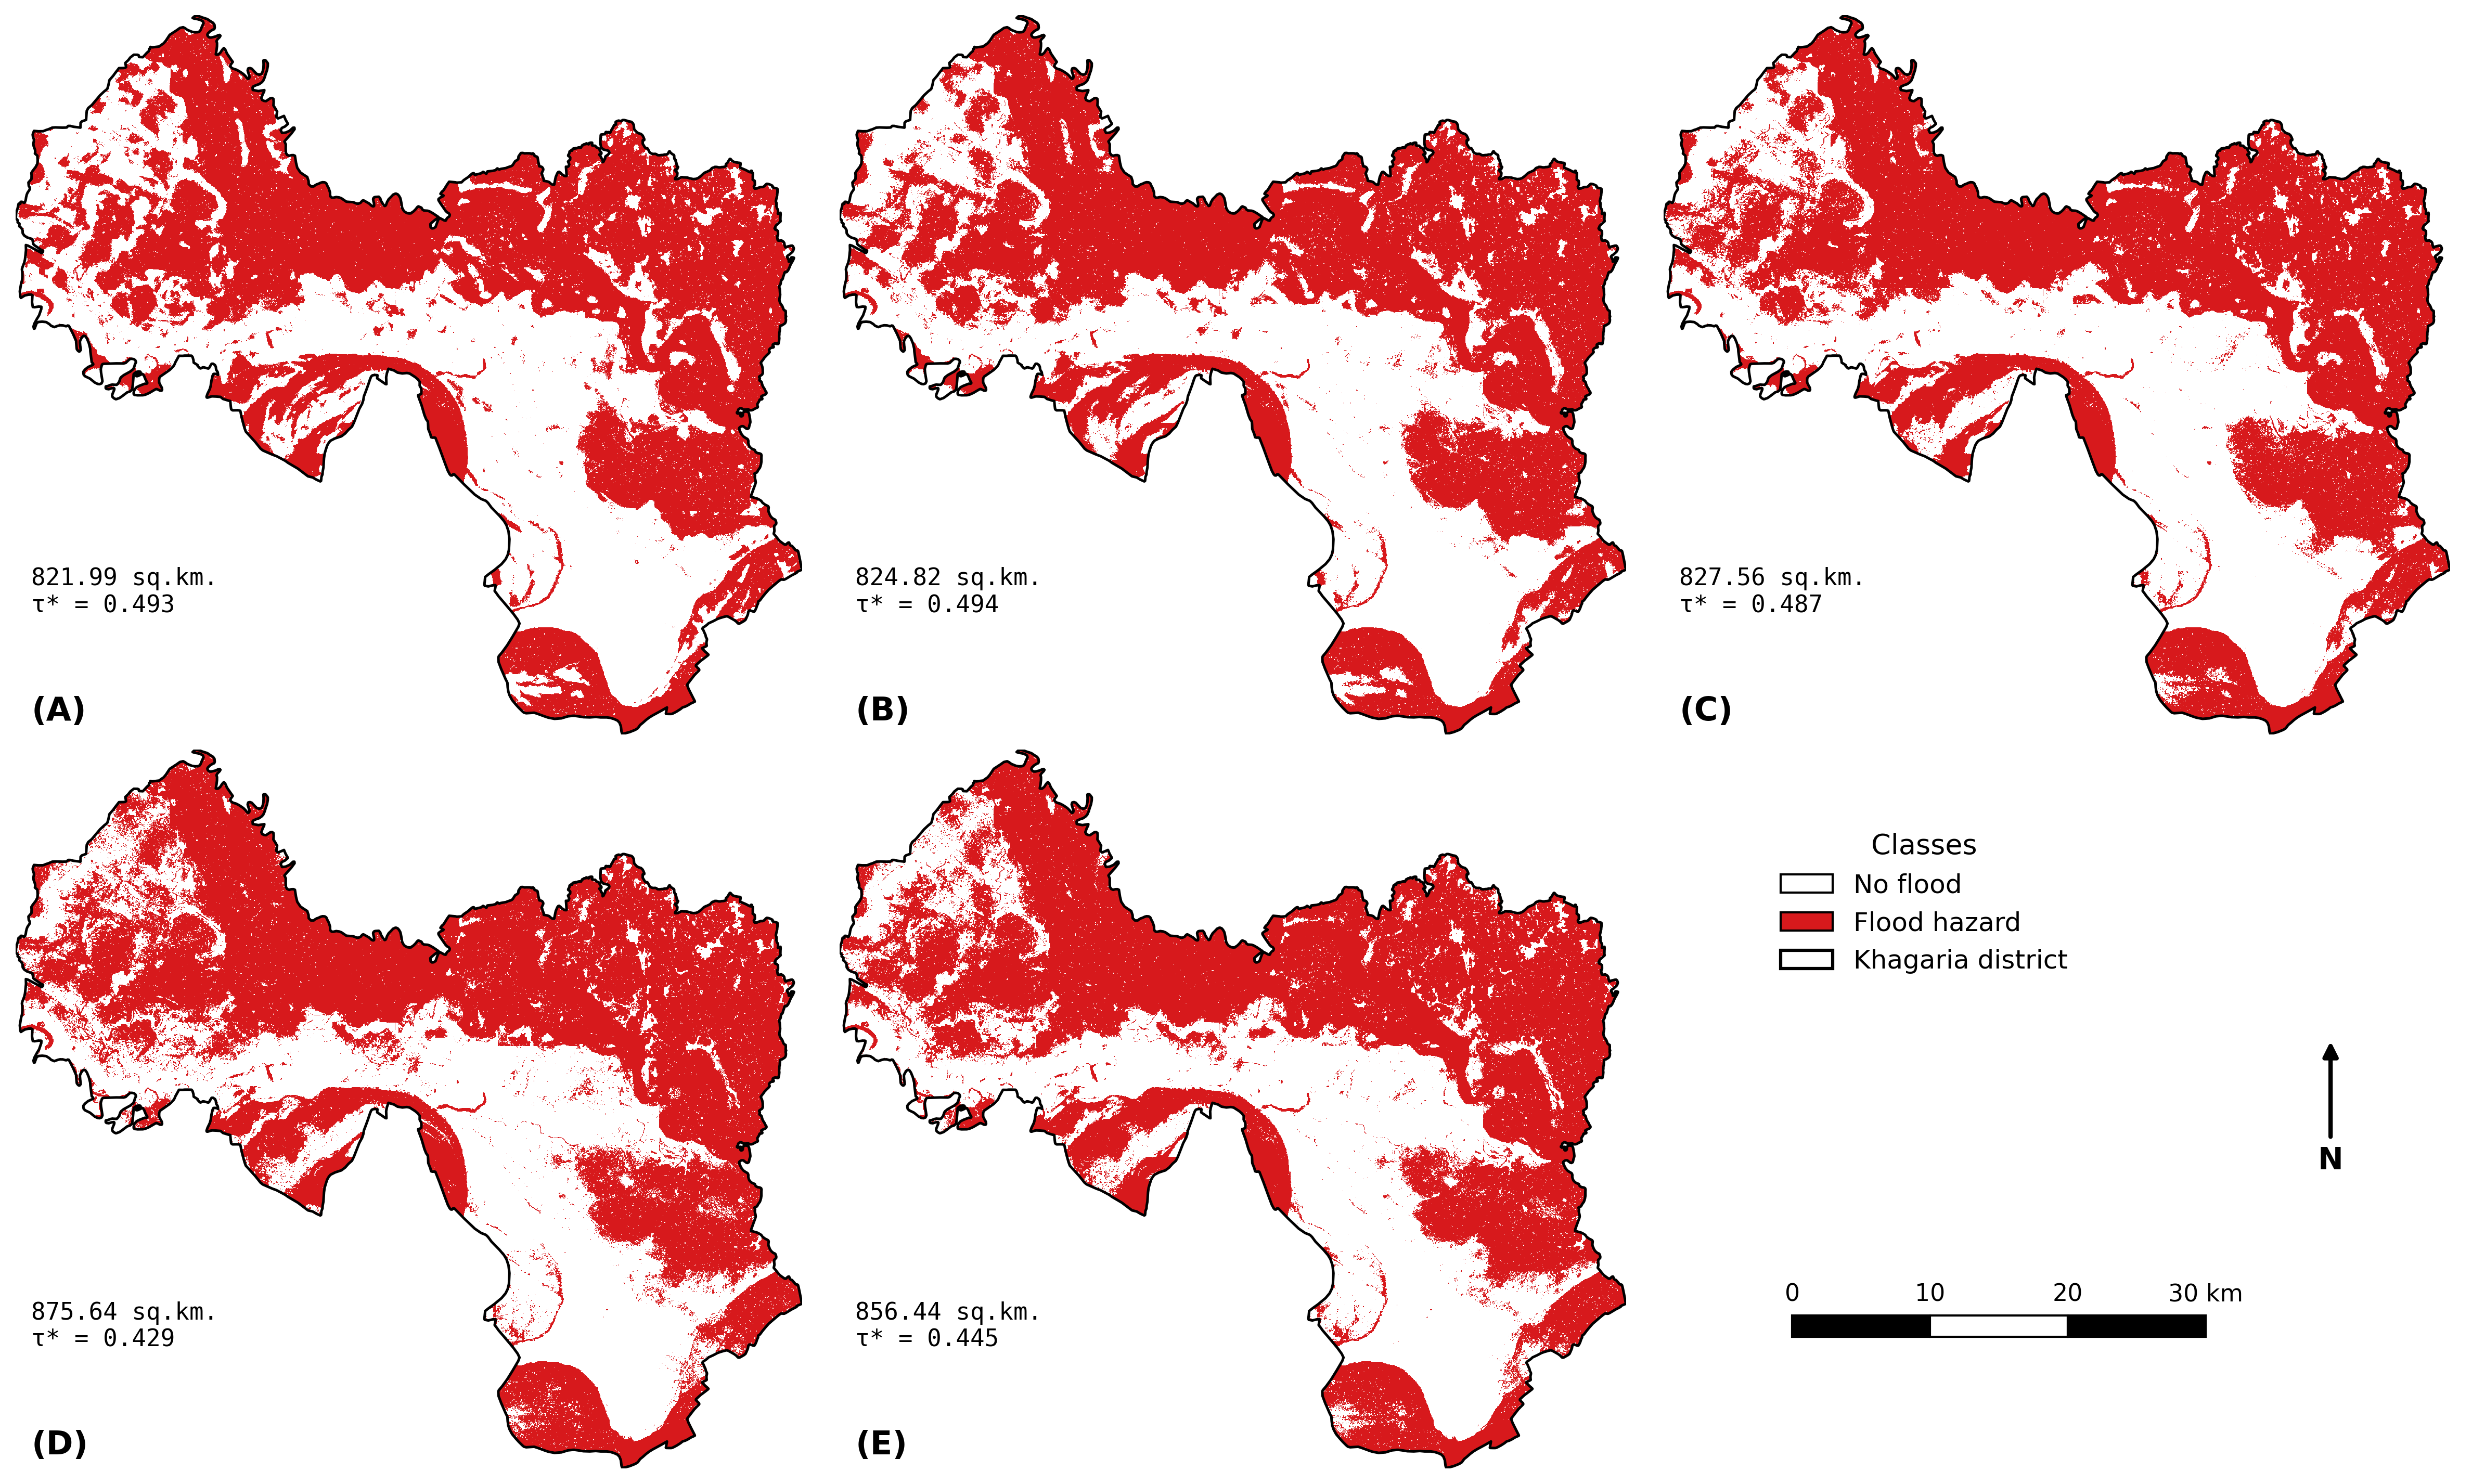
\includegraphics[width=\textwidth]{Figures_v2/FHM.png}
    \caption{Binary flood hazard maps (FHMs) for all five models at their Max-CSI thresholds ($\tau^*$, chosen on the validation set). (A) XGBoost ($\tau^* = 0.493$, flood area = 821.99 km\textsuperscript{2}); (B) CatBoost ($\tau^* = 0.494$, 824.82 km\textsuperscript{2}); (C) RandomForest ($\tau^* = 0.487$, 827.56 km\textsuperscript{2}); (D) ANN ($\tau^* = 0.429$, 875.64 km\textsuperscript{2}); (E) DNN ($\tau^* = 0.446$, 856.44 km\textsuperscript{2}). Red = Flood Hazard Zone; White = Safe Zone. The three tree-based models give flood extents of 822--828 km\textsuperscript{2}, close to the inventory extent of 824.4 km\textsuperscript{2}; the neural networks give 856--876 km\textsuperscript{2}.}
    \label{fig:fhm}
\end{figure}

The tree-based FHMs (Figure~\ref{fig:fhm}A--C) cover 821.99, 824.82, and 827.56 km\textsuperscript{2} (XGBoost, CatBoost, RF) --- a range of 5.6 km\textsuperscript{2} around the inventory extent of 824.4 km\textsuperscript{2}. The DNN and ANN FHMs cover 856.44 and 875.64 km\textsuperscript{2}, 4--6\% more than the inventory, because their lower thresholds trade specificity for sensitivity (Table~\ref{tab:results}). Where the models agree, they agree strongly: all five flag the same 734.4 km\textsuperscript{2} as hazard and none flags 519.4 km\textsuperscript{2}, so 85.4\% of the district receives the same class from every model, and only 215.3 km\textsuperscript{2} (14.7\%) is disputed.

\subsection{Susceptibility Class Area Statistics}

Table~\ref{tab:area} presents the share of the district (1,469.0 km\textsuperscript{2} of valid pixels) in each susceptibility class for all five FSMs. XGBoost assigns 47.0\% of the district to the Very High class and 34.4\% to Very Low, leaving only 18.6\% in the three intermediate classes. The other models spread more area over the intermediate classes (31.9\%--42.8\%), with Very High shares between 33.7\% (ANN) and 41.3\% (CatBoost).

\begin{table}[H]
\centering
\caption{Percentage of the district area (1,469.0 km\textsuperscript{2} of valid pixels) in each flood susceptibility class (natural breaks computed on the XGBoost map) for each model.}
\label{tab:area}
\begin{adjustbox}{max width=\linewidth}
\begin{tabular}{lccccc}
\toprule
\textbf{Model} & \textbf{Very Low (\%)} & \textbf{Low (\%)} & \textbf{Moderate (\%)} & \textbf{High (\%)} & \textbf{Very High (\%)} \\
\midrule
XGBoost      & 34.35 & 7.40  & 4.61  & 6.63  & 47.02 \\
CatBoost     & 28.48 & 11.14 & 8.42  & 10.62 & 41.33 \\
RandomForest & 22.11 & 15.79 & 12.08 & 14.29 & 35.73 \\
ANN          & 23.48 & 13.39 & 13.17 & 16.23 & 33.73 \\
DNN          & 23.49 & 14.02 & 12.49 & 14.04 & 35.96 \\
\end{tabular}
\end{adjustbox}
\end{table}

%% ============================================================
%%  5. DISCUSSION
%% ============================================================
\section{Discussion}

\subsection{Physical Interpretation of SHAP-Derived Feature Importance}
\label{sec:disc_shap}

The SHAP analysis shows that all five models rely on the same small set of factors. Rainfall, Geomorphology, Soil, and Elevation occupy the top four ranks in every model, and their consistency across very different learners indicates that the models have captured stable relationships in the data rather than artefacts of one algorithm.

\paragraph{Geomorphology as the dominant integrative predictor.}
Geomorphology ranks first or second in all five models (normalised score 0.975--1.000). It acts as an integrated, process-aware landform classifier that encodes information unavailable to any single topometric index: \textit{chaur} depressions trap monsoon and backwater inundation, whereas natural levees and older alluvial terraces flood only in extreme events. This finding is consistent with the geomorphic flood index framework of \citet{samela2017} and with the geomorphological controls documented for Bihar floods \citep{sinha2008}, and supports the view that landform classification subsumes much of the predictive content of terrain derivatives in near-flat alluvial environments.

\paragraph{Soil type: the infiltration--runoff switch.}
Soil ranks first in RF, ANN, and DNN and second or third in the boosted models. It marks the threshold between infiltration-dominated and runoff-dominated response: fine-textured alluvial clays on the floodplain surface saturate quickly and then generate direct runoff, while sandy loams on levee crests and \textit{diara} land keep higher infiltration capacities through the monsoon \citep{NBSSLUPbihar2020}. Because the soil layer is mapped at about 1 km, its unit boundaries also imprint straight edges on the susceptibility maps; a finer soil map would remove this artefact.

\paragraph{Rainfall: physical trigger or location proxy?}
Rainfall ranks first in XGBoost and third or fourth elsewhere. Monsoon precipitation is the primary trigger of the synchronised river peaks that flood Khagaria, but within a single district the long-term mean rainfall field varies by only 155 mm and changes smoothly with position. A smooth regional field of this kind can serve the models as a coordinate, separating the north of the district (Kosi belt) from the centre. Its high SHAP rank should therefore not be read as evidence that pixel-level rainfall differences cause the flood pattern; event rainfall or discharge would be needed to test that.

\paragraph{Model-specificity of importance profiles.}
The rank heatmap (Figure~\ref{fig:shap_heatmap}) shows that the models differ mainly in the order of the top four and of the second tier (Distance to Roads, Stream Density, Distance to Stream, LULC). XGBoost gives more weight to Rainfall and Distance to Roads, whereas RF and the neural networks give more weight to Soil and LULC. ANN and DNN have almost identical rankings.

\paragraph{Terrain derivatives: low importance in flat terrain.}
TWI, Slope, Aspect, and Curvature rank 11--14 in every model. In terrain where the SRTM slope is dominated by vertical quantisation and noise, these derivatives carry little information beyond Elevation and Geomorphology. Flood susceptibility studies in similar alluvial settings that include all SRTM-derived indices without checking their importance risk adding noise predictors \citep{tehrany2019, khosravi2018}.

\subsection{Why Tree-Based Models Outperform Deep Learning on Tabular Geospatial Data}

The results agree with the tabular-data benchmarks \citep{grinsztajn2022, shwartzziv2022, mcelfresh2023}: gradient-boosted trees outperform the neural architectures on this structured, medium-dimensional dataset. The CSI gap between XGBoost (0.923) and the best neural network, DNN (0.804), is 0.119 points, and the AUC gap is 0.041.

The most direct explanation is inductive bias \citep{Mitchell1980}. Flood susceptibility in alluvial plains is largely governed by threshold-type rules on individual factors --- a pixel is at risk if it lies in a particular landform or soil unit, below a critical elevation, or within a certain distance of a channel. Axis-aligned conditions of this kind are what recursive binary partitioning in decision trees represents \citep{breiman2001}, whereas neural networks with smooth activations favour smooth decision surfaces \citep{Popov2021}. The four most important factors here include two categorical maps (Geomorphology and Soil) entered as integer codes, which trees can split directly but which a neural network must approximate with smooth functions of an arbitrary code order; one-hot encoding of these factors would be a fairer test for the neural networks. Notably, the weaker performance of ANN and DNN is not a calibration problem: their probabilities are the best calibrated of the five models (ECE 0.013--0.014), and their optimal thresholds (0.43--0.45) are only moderately below 0.5. Their wider hazard maps (856--876 km\textsuperscript{2}) follow from lower discrimination, which forces the CSI-optimal threshold to trade specificity for sensitivity.

Where DL does excel in hydrology is in tasks with fundamentally different structural properties. Long Short-Term Memory networks and Transformer architectures applied to time-series streamflow forecasting \citep{Kratzert2018, Frame2022} leverage temporal autocorrelation and sequential process dynamics across thousands of basin-hours of training data. Large-scale weather prediction models \citep{Bi2023, Lam2023} exploit the high spatial dimensionality of gridded atmospheric fields. The key discriminating factor is data structure: DL is the appropriate choice when inputs are high-dimensional (images, time series, gridded fields), whereas tree ensembles are the more reliable default for tabular classification with a small set of handcrafted features \citep{mcelfresh2023, shwartzziv2022}. Flood susceptibility mapping with 10--20 terrain-derived attributes per pixel falls in the latter category.

Data scale and tuning effort also matter. The training set here contains 1.14 million pixels, but they are strongly spatially autocorrelated, so the effective number of independent samples is much smaller \citep{roberts2017}. Dropout and batch normalisation regularise the networks, but ensemble methods achieve efficient implicit regularisation through bootstrap sampling and feature subsampling \citep{dietterich2000, breiman2001}. These findings are consistent with geohazard-specific evidence: \citet{Arabameri2021} found XGBoost superior to ANN in gully erosion susceptibility; \citet{Iban2022} reported CatBoost outperforming DL for landslide susceptibility; \citet{zhang2022} demonstrated XGBoost dominance in multi-hazard susceptibility frameworks; and \citet{Arora2024Argens} showed that RF and XGBoost outperformed ANN when benchmarked against high-resolution hydrodynamic flood hazard maps over the Argens Basin, France. For geospatial hazard susceptibility mapping with conventional CgF inputs, tree-based ensembles are a sound default choice.

\subsection{Max-CSI Thresholding and Operational Hazard Map Quality}

Max-CSI gave a higher test CSI than Youden's Index for all five models, although the gain was small (mean $\Delta\text{CSI} = +0.0048$). The size of the gain depends on the setting. Here the flood class covers 56\% of the district and the probabilities are reasonably calibrated, so the CSI curve is flat around 0.5 and every sensible threshold performs similarly; the fixed 0.5 cut-off is within 0.0035 CSI of Max-CSI for every model. Larger gains are expected where floods are rare or probabilities are poorly calibrated, which is the usual situation in flood susceptibility studies \citep{tehrany2019, Costache2020, Arora2022SERRA}. The general argument for Max-CSI is that it states the operational objective explicitly: the CSI ignores true negatives and penalises both missed floods and false alarms \citep{schaefer1990, mason2003}, so the threshold is chosen for flood detection rather than for overall accuracy. Choosing the threshold on a validation split, as done here, also keeps the reported test CSI free of selection bias.

The close agreement between the XGBoost FHM extent (821.99 km\textsuperscript{2}) and the inventory extent (824.4 km\textsuperscript{2}) should be interpreted with care: because maximising the CSI pushes false-positive and false-negative counts towards balance, CSI-optimal thresholding pulls the predicted flood area towards the reference area, so extent agreement is partly a property of the criterion rather than independent validation. The more informative result is the pixel-level agreement: XGBoost misclassifies 4.5\% of test pixels (CSI 0.923), and the five models agree on 85.4\% of the district. The neural networks overestimate the extent by 4--6\% at their CSI-optimal thresholds, reflecting their weaker discrimination.

\subsection{Bihar Floods and the Upper North Bihar Crisis Zone}

The derived XGBoost FHM spatially resolves flood dynamics that are qualitatively well-understood in the Bihar flood literature but have not previously been mapped at pixel-level resolution using ML methods. High-hazard zones trace the Kosi meander belt, the Burhi Gandak corridor, and the Ganga backwater zone with precision that closely mirrors historical flood damage records \citep{bhuvan2010, tatatrusts2024, sinha2008, Arora2025SciRep, Arora2022SERRA}. The model's delineation of \textit{chaur} depressions as distinct high-hazard polygons sharply separated from safer levee ridges resolves sub-kilometre geomorphological features operationally critical for waterlogging risk assessment but absent from coarser official flood atlases \citep{bhuvan2010}.

The upper North Bihar region --- spanning the Himalayan foothills and the immediate flood-receiving districts of Darbhanga, Sitamarhi, Madhubani, Supaul, and Saharsa in addition to Khagaria --- constitutes one of the most consistently and severely flood-affected corridors on Earth. The driving mechanism is structurally embedded: the Kosi, Bagmati, Gandak, and Kamla Balan all originate in Nepal's Himalayas, where snowmelt and concentrated monsoon precipitation generate simultaneous peak discharges that arrive on the Bihar plains within days of each other \citep{sinha2008, mishra2018, Jha2012, Costache2021Geocarto}. The Kosi's extraordinary sedimentation rate --- approximately 100--150 million tonnes annually \citep{sinha2008} --- has progressively raised its bed above the surrounding floodplain, making it a perched, above-grade river structurally prone to avulsion. The 2008 Kusaha breach, in which the Kosi shifted its course by approximately 120 km in days and inundated over 3,400 km\textsuperscript{2} of Bihar, is the most extreme recent manifestation of this dynamic \citep{bhuvan2010, mishra2018}. The embankment system constructed since the 1950s has, paradoxically, accelerated bed aggradation within embankments and transferred catastrophic breach risk to downstream districts like Khagaria \citep{beams2024, mishra2018}. ML susceptibility studies of the type conducted here --- operating at pixel level with multi-year SAR-calibrated inventories --- are uniquely positioned to resolve the spatial heterogeneity of this hazard within individual districts. Identification of specific blocks (Parbatta, Gogri, Alauli, Beldaur, Mansi) and landscape elements (\textit{chaurs}, river confluence zones, backwater-prone areas) as consistently high-hazard provides the DDMA with spatial precision needed for targeted embankment reinforcement, early warning system placement, and pre-monsoon evacuation planning. Extension of this methodology to the full upper North Bihar crisis zone --- integrating dynamic variables such as Kosi discharge at Bhimnagar barrage, Sentinel-1-derived soil moisture, and SWOT water surface elevations \citep{Biancamaria2016} --- represents a tractable and high-impact direction for future operational flood forecasting in one of the world's most vulnerable river systems.

\subsection{Spatial Implications and Comparison with Official Assessments}

The pixel-level hazard resolution of the XGBoost FHM is a material improvement over existing official flood hazard atlases \citep{bhuvan2010} that classify hazard at block level. The XGBoost map delineates intra-block heterogeneity at 30 m --- identifying elevated levee ridges along the Kosi and Burhi Gandak as locally safe corridors within otherwise high-hazard blocks, and distinguishing the variable susceptibility of the Parbatta block (where Kosi and Kareh channels produce contrasting micro-topographic flood exposure) from the uniformly high-hazard character of Mansi and Alauli blocks at the Ganga confluence. This spatial detail is operationally relevant for siting flood shelters, planning evacuation routes, and prioritising infrastructure protection. The three tree-based models converge on 822--828 km\textsuperscript{2} ($\approx$56\% of the district) as flood hazard, and all five models agree on the class of 85.4\% of the district, which supports confidence in the hazard delineation. The 14.7\% of the district on which the models disagree marks where field verification would be most useful.

The XGBoost threshold ($\tau^* = 0.493$) is close to 0.5, and all five models have thresholds between 0.43 and 0.50. In this study the choice of threshold therefore matters less than the choice of model; in settings with rarer floods or less well calibrated models, threshold validation becomes more important and should be part of any flood susceptibility study intended for operational use.

\subsection{Limitations and Future Directions}

Several limitations merit acknowledgement. First, and most importantly from a validation standpoint, the train / validation / test partition used stratified \textit{random pixel-level} sampling. Because conditioning factors are strongly spatially autocorrelated at 30 m resolution, test pixels frequently neighbour training pixels in both geographic and feature space; the reported accuracy metrics therefore measure \textit{interpolative} skill within the district and are likely optimistic with respect to transfer to unseen regions or events \citep{roberts2017, ploton2020}. Spatially blocked cross-validation, in which entire contiguous zones are withheld, is the appropriate protocol for estimating extrapolative performance and is a priority for follow-up work. This inflation affects all five models in the same way and therefore does not alter the comparative conclusions or the threshold comparison, which are within-design contrasts. Second, the inventory is the union of three events and labels every non-flooded pixel as safe; pixels that flood in other events (1987, 2004, 2024) are labelled non-flood, so the models learn the observed flood envelope rather than a return-period hazard. Third, the equal-effort configuration protocol means that no model was exhaustively tuned, and the categorical factors were entered as integer codes; one-hot encoding and a deeper hyperparameter search could narrow the gap between the neural networks and the trees, although tabular benchmarks indicate that tuned deep models rarely overtake tuned gradient-boosted trees at this scale \citep{grinsztajn2022, shwartzziv2022, mcelfresh2023}. Fourth, several inputs are coarser than the 30 m grid: the soil map (about 1 km) imprints straight unit boundaries on the maps, and the rainfall field is smooth enough to act partly as a location variable. Fifth, the study relies on 30 m SRTM elevation data, which cannot resolve micro-topographic features --- irrigation canal embankments, road beds, settlement mounds --- that locally modulate inundation at sub-50 m scales \citep{neal2021, Hawker2022}; in this flat terrain the SRTM slope is dominated by quantisation and noise. Integration of LiDAR or Cartosat-3 DEM would substantially enhance spatial precision, particularly for \textit{diara} ridge delineation and road-bounded drainage compartments. The static CgF-based model treats terrain as fixed, precluding direct application to event-specific forecasting where antecedent soil moisture, real-time discharge, and embankment integrity dominate \citep{sinha2008, mishra2018}. Future work should integrate near-real-time hydrological variables --- CWC gauge data, SWOT water surface elevations \citep{Biancamaria2016}, and Sentinel-1 soil moisture --- within an XGBoost or CatBoost framework for dynamic, event-specific flood probability maps. A particularly promising direction to overcome the current data limitation is the use of hydraulic model outputs as the training target. A two-dimensional hydrodynamic simulation (e.g., HEC-RAS 2D, LISFLOOD-FP, or ANUGA) calibrated to the Kosi--Ganga system and run for standard return-period scenarios --- 100-year, 500-year, and 1,000-year recurrence intervals --- would provide physically rigorous inundation extents as target rasters \citep{teng2017, Bates2010}. Training an XGBoost or CatBoost model on these synthetic hydraulic targets would let the ML framework learn extreme-event flood dynamics not yet observed in the multi-event SAR inventory, and would align ML susceptibility products with the return-period framework already used by engineers and planners \citep{neal2021, teng2017}.

Additional directions include LightGBM \citep{ke2017} as a complementary tree-based competitor, one-hot or embedding encodings of the categorical factors for the neural networks, and Transformer-based tabular architectures \citep{Gorishniy2021} as the DL frontier evolves.

%% ============================================================
%%  6. CONCLUSION
%% ============================================================
\section{Conclusion}

This study presented a multi-model comparison of ML and DL approaches for flood susceptibility mapping and FHM derivation in Khagaria district, Bihar --- one of India's most persistently flood-affected districts, situated at the convergence of seven major Himalayan and peninsular river systems. A multi-year multi-mission SAR flood inventory --- ENVISAT ASAR (2008) and Sentinel-1 (2020, 2021) --- covering 824.4 km\textsuperscript{2} (56.1\%) of the modelled district was combined with fourteen non-collinear conditioning factors (maximum VIF 1.82), and five models were trained and evaluated with separate training, validation, and test splits.

XGBoost achieved the highest performance on the independent test set (AUC = 0.9920; CSI = 0.9229; Sensitivity = 0.9586; Specificity = 0.9504; $\tau^* = 0.493$), followed by CatBoost (AUC = 0.9794; CSI = 0.8731) and RF (AUC = 0.9708; CSI = 0.8483), while DNN and ANN yielded lower CSI values of 0.804 and 0.795. The advantage of the tree-based models is consistent with their inductive bias for the axis-aligned, threshold-type decision boundaries that govern alluvial flood inundation, and with the categorical nature of the two most important factors. The neural networks were the best-calibrated models (ECE 0.013--0.014), so their lower CSI reflects weaker discrimination rather than miscalibration.

Max-CSI threshold optimisation gave a higher test CSI than Youden's Index for all five models, by a small margin (mean $\Delta\text{CSI} = +0.0048$), because the near-balanced inventory and reasonably calibrated probabilities make the CSI curve flat around 0.5. The XGBoost FHM at $\tau^* = 0.493$ covers 821.99 km\textsuperscript{2} (56.0\% of the district), and all five models agree on the class of 85.4\% of the district. Rainfall, Geomorphology, Soil, and Elevation are the four dominant predictors in every model, with the caveat that the smooth rainfall field partly acts as a location variable. The FHM resolves intra-district flood heterogeneity at 30 m --- identifying the Kosi meander belt, Burhi Gandak corridor, Ganga backwater zone, and \textit{chaur} depressions as high-hazard zones --- and is a substantially finer product than existing block-level official assessments. The XGBoost FSM assigns 47.0\% of Khagaria's area to the Very High susceptibility class, providing the DDMA with spatial targeting for embankment reinforcement, shelter siting, and evacuation planning.

Future priorities include spatially blocked validation, dynamic integration of real-time hydrological variables for event-specific forecasting, higher-resolution elevation and soil data (LiDAR/Cartosat-3; detailed soil surveys), extension of the multi-year inventory to include the 1987, 2004, and 2024 floods, and scaling the methodology to the full upper North Bihar crisis zone for comprehensive district-level flood risk governance.

%% ============================================================
%%  DECLARATIONS
%% ============================================================

\section*{Statements and Declarations}

%
%
%
\subsection*{Funding}
The first author is supported by the Marie Sk\l odowska-Curie COFUND Fellowship through the SMASH programme, co-funded by the European Union's Horizon Europe Research and Innovation Programme under Grant Agreement No.\ 101081355. The funder had no role in study design, data collection and analysis, decision to publish, or preparation of the manuscript.

\subsection*{Competing Interests}
The authors declare that they have no competing financial interests or personal relationships that could have influenced the work reported in this paper.

\subsection*{Data Availability}
The input rasters, flood inventory, trained models, analysis scripts, and all results (metrics, curves, SHAP values, and maps) are held in a GitHub repository (\url{https://github.com/ami01/khagaria-fhm}) \textcolor{red}{[currently private; make public and archive on Zenodo with a DOI before publication, or revert to ``available on request'']}. Sentinel-1 SAR imagery is publicly available through the Copernicus Data Space Ecosystem (\url{https://dataspace.copernicus.eu}).

\subsection*{Ethics Approval}
Not applicable. This study did not involve human participants or animals.

\section*{Acknowledgements}
The first author is supported by the Marie Sklodowska-Curie COFUND Fellowship through the SMASH programme (European Union's Horizon Europe Research and Innovation Programme, Grant Agreement No. 101081355) at the University of Nova Gorica, hosted at the Slovenian Environment Agency (ARSO). The authors acknowledge the
Flood Management Information System Centre (FMISC), Water Resources Department, Government of Bihar, for providing district-level hydrological baseline data. Sentinel-1 data were obtained from the European Space Agency Copernicus Programme free of charge.

%% ============================================================
%%  REFERENCES
%% ============================================================
\newpage
\bibliographystyle{abbrvnat}
\bibliography{references}



%% ============================================================
%%  SUPPLEMENTARY MATERIAL
%% ============================================================
\newpage
\section*{Supplementary Material}

\setcounter{figure}{0}
\renewcommand{\thefigure}{S\arabic{figure}}
\setcounter{table}{0}
\renewcommand{\thetable}{S\arabic{table}}

\begin{figure}[H]
  \centering
  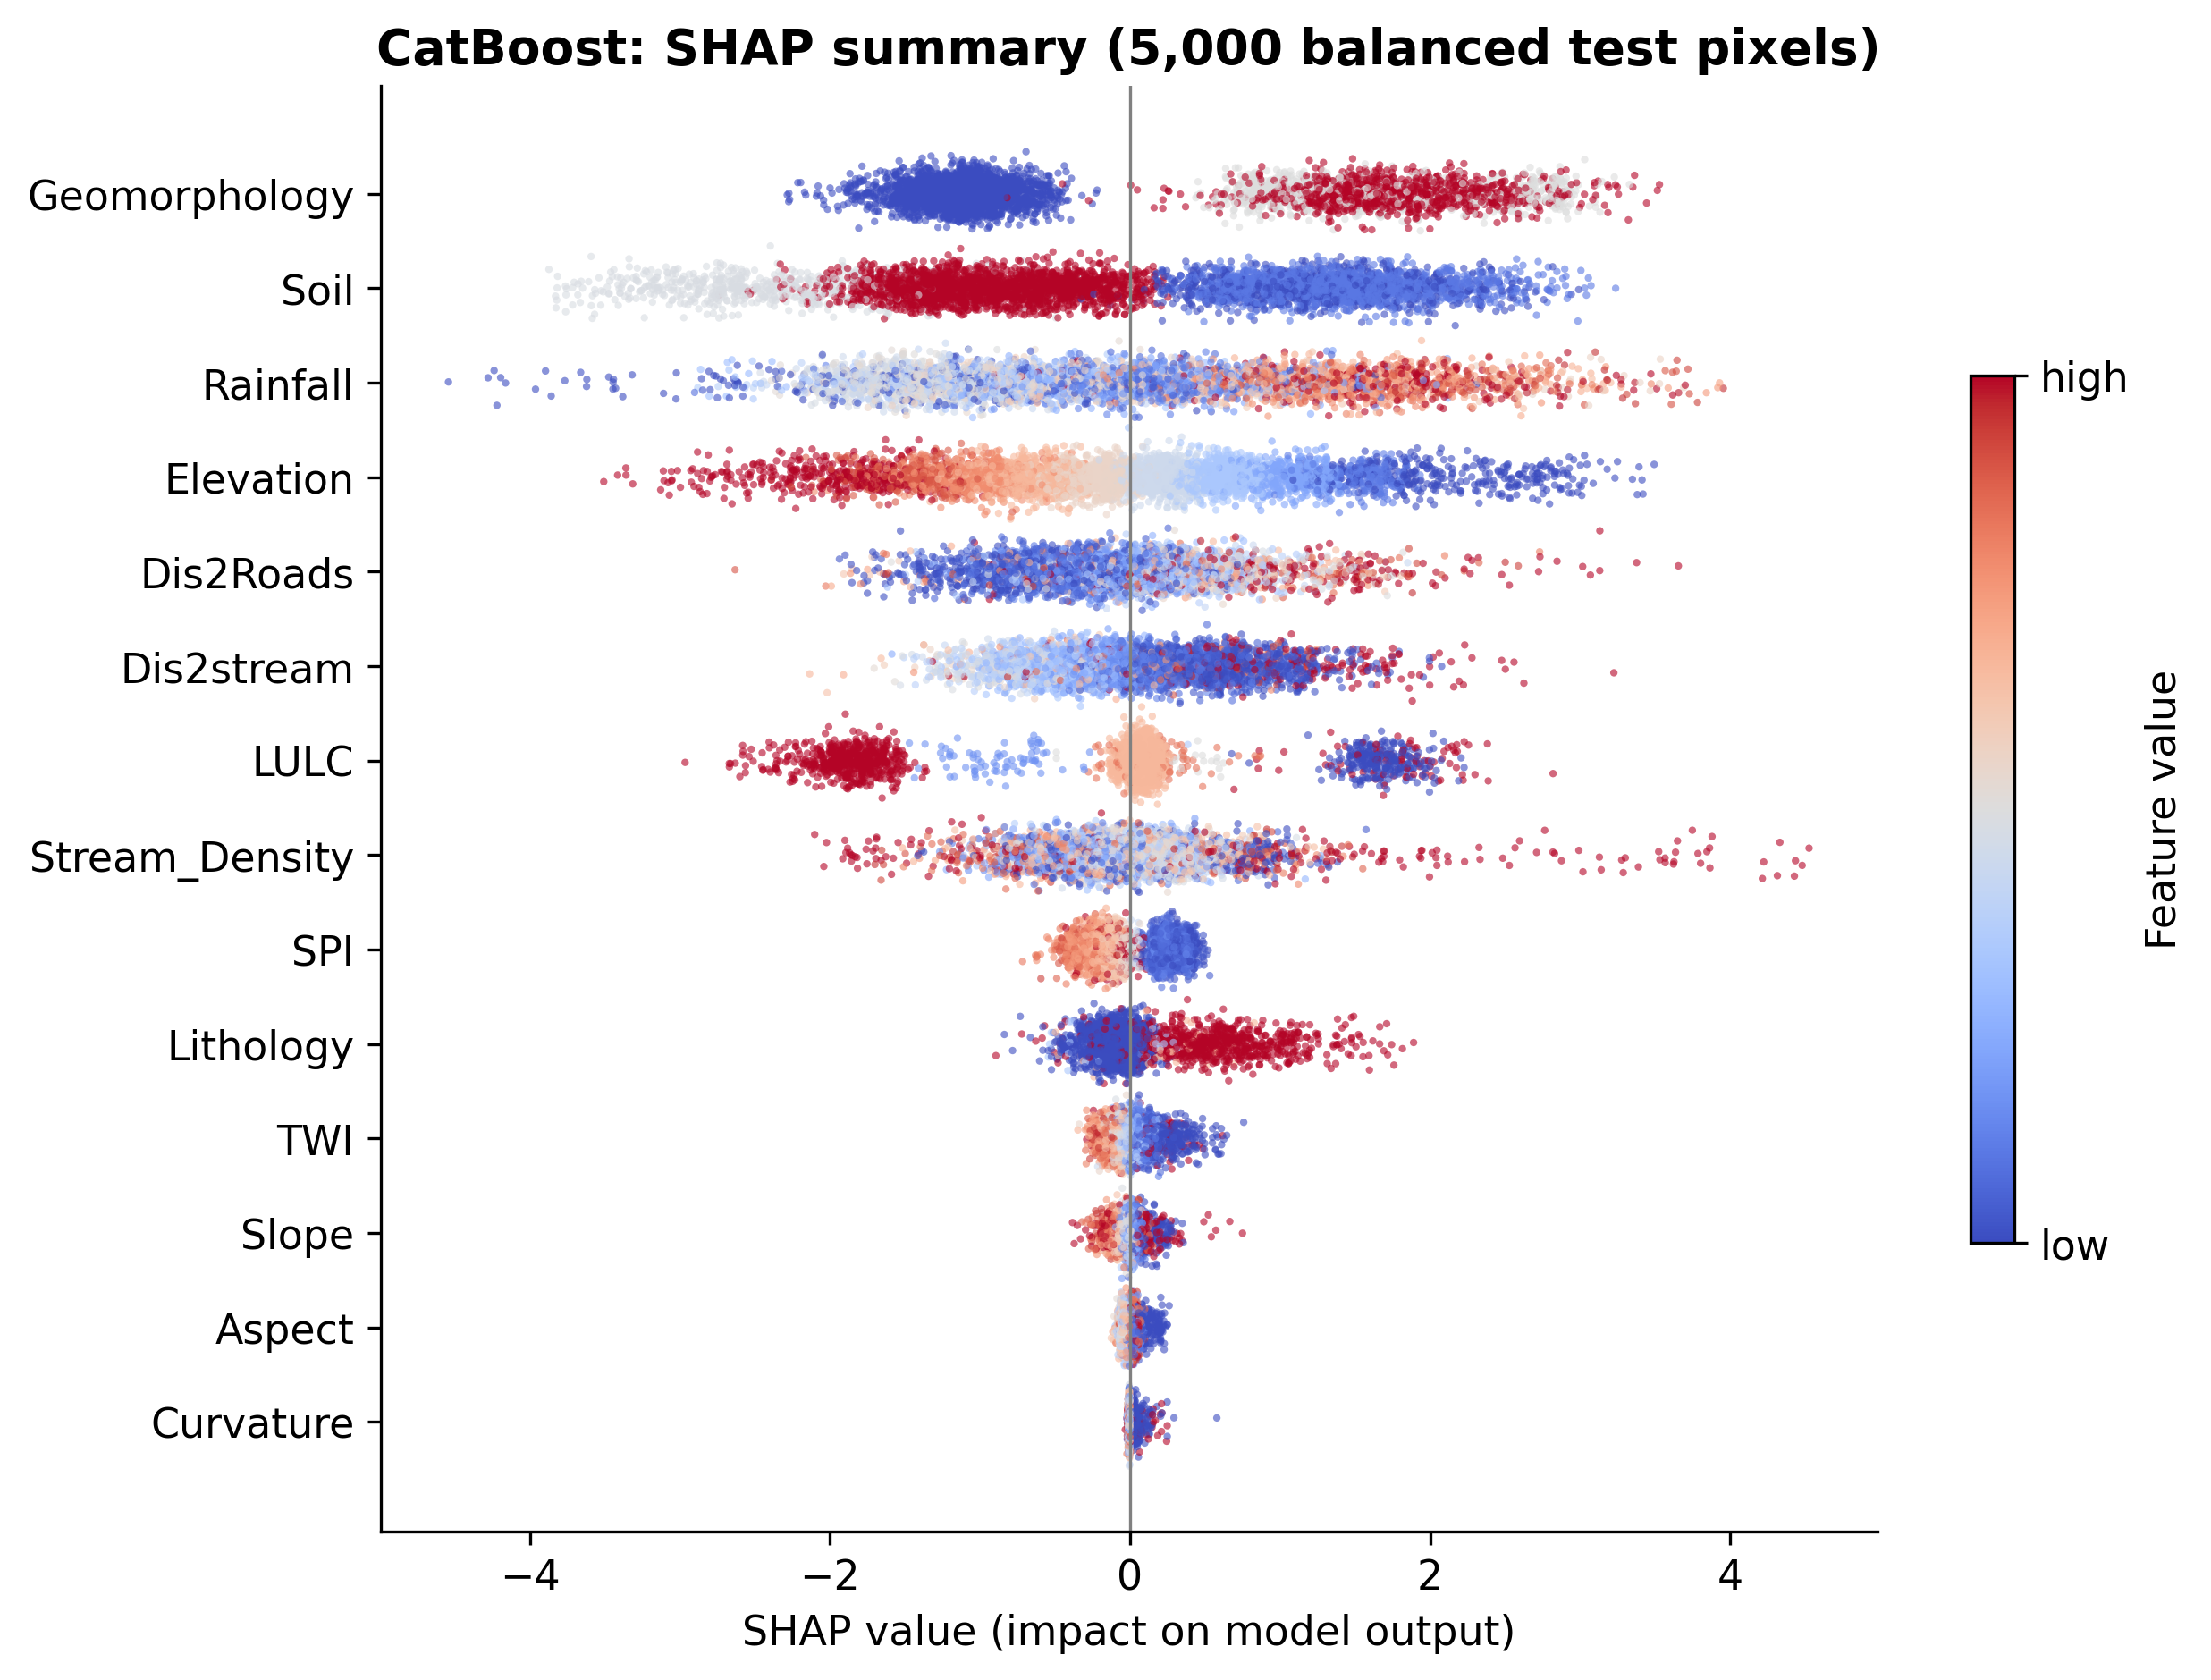
\includegraphics[width=0.85\textwidth]{Figures_v2/Fig_SHAP_Beeswarm_CatBoost.png}
  \caption{CatBoost SHAP beeswarm plot (5,000 balanced test pixels). Geomorphology ranks first, followed by Soil, Rainfall, and Elevation --- the same top four as XGBoost (Figure~\ref{fig:shap_beeswarm_xgb}) in a different order.}
  \label{fig:shap_beeswarm_cat}
\end{figure}

\begin{figure}[H]
  \centering
  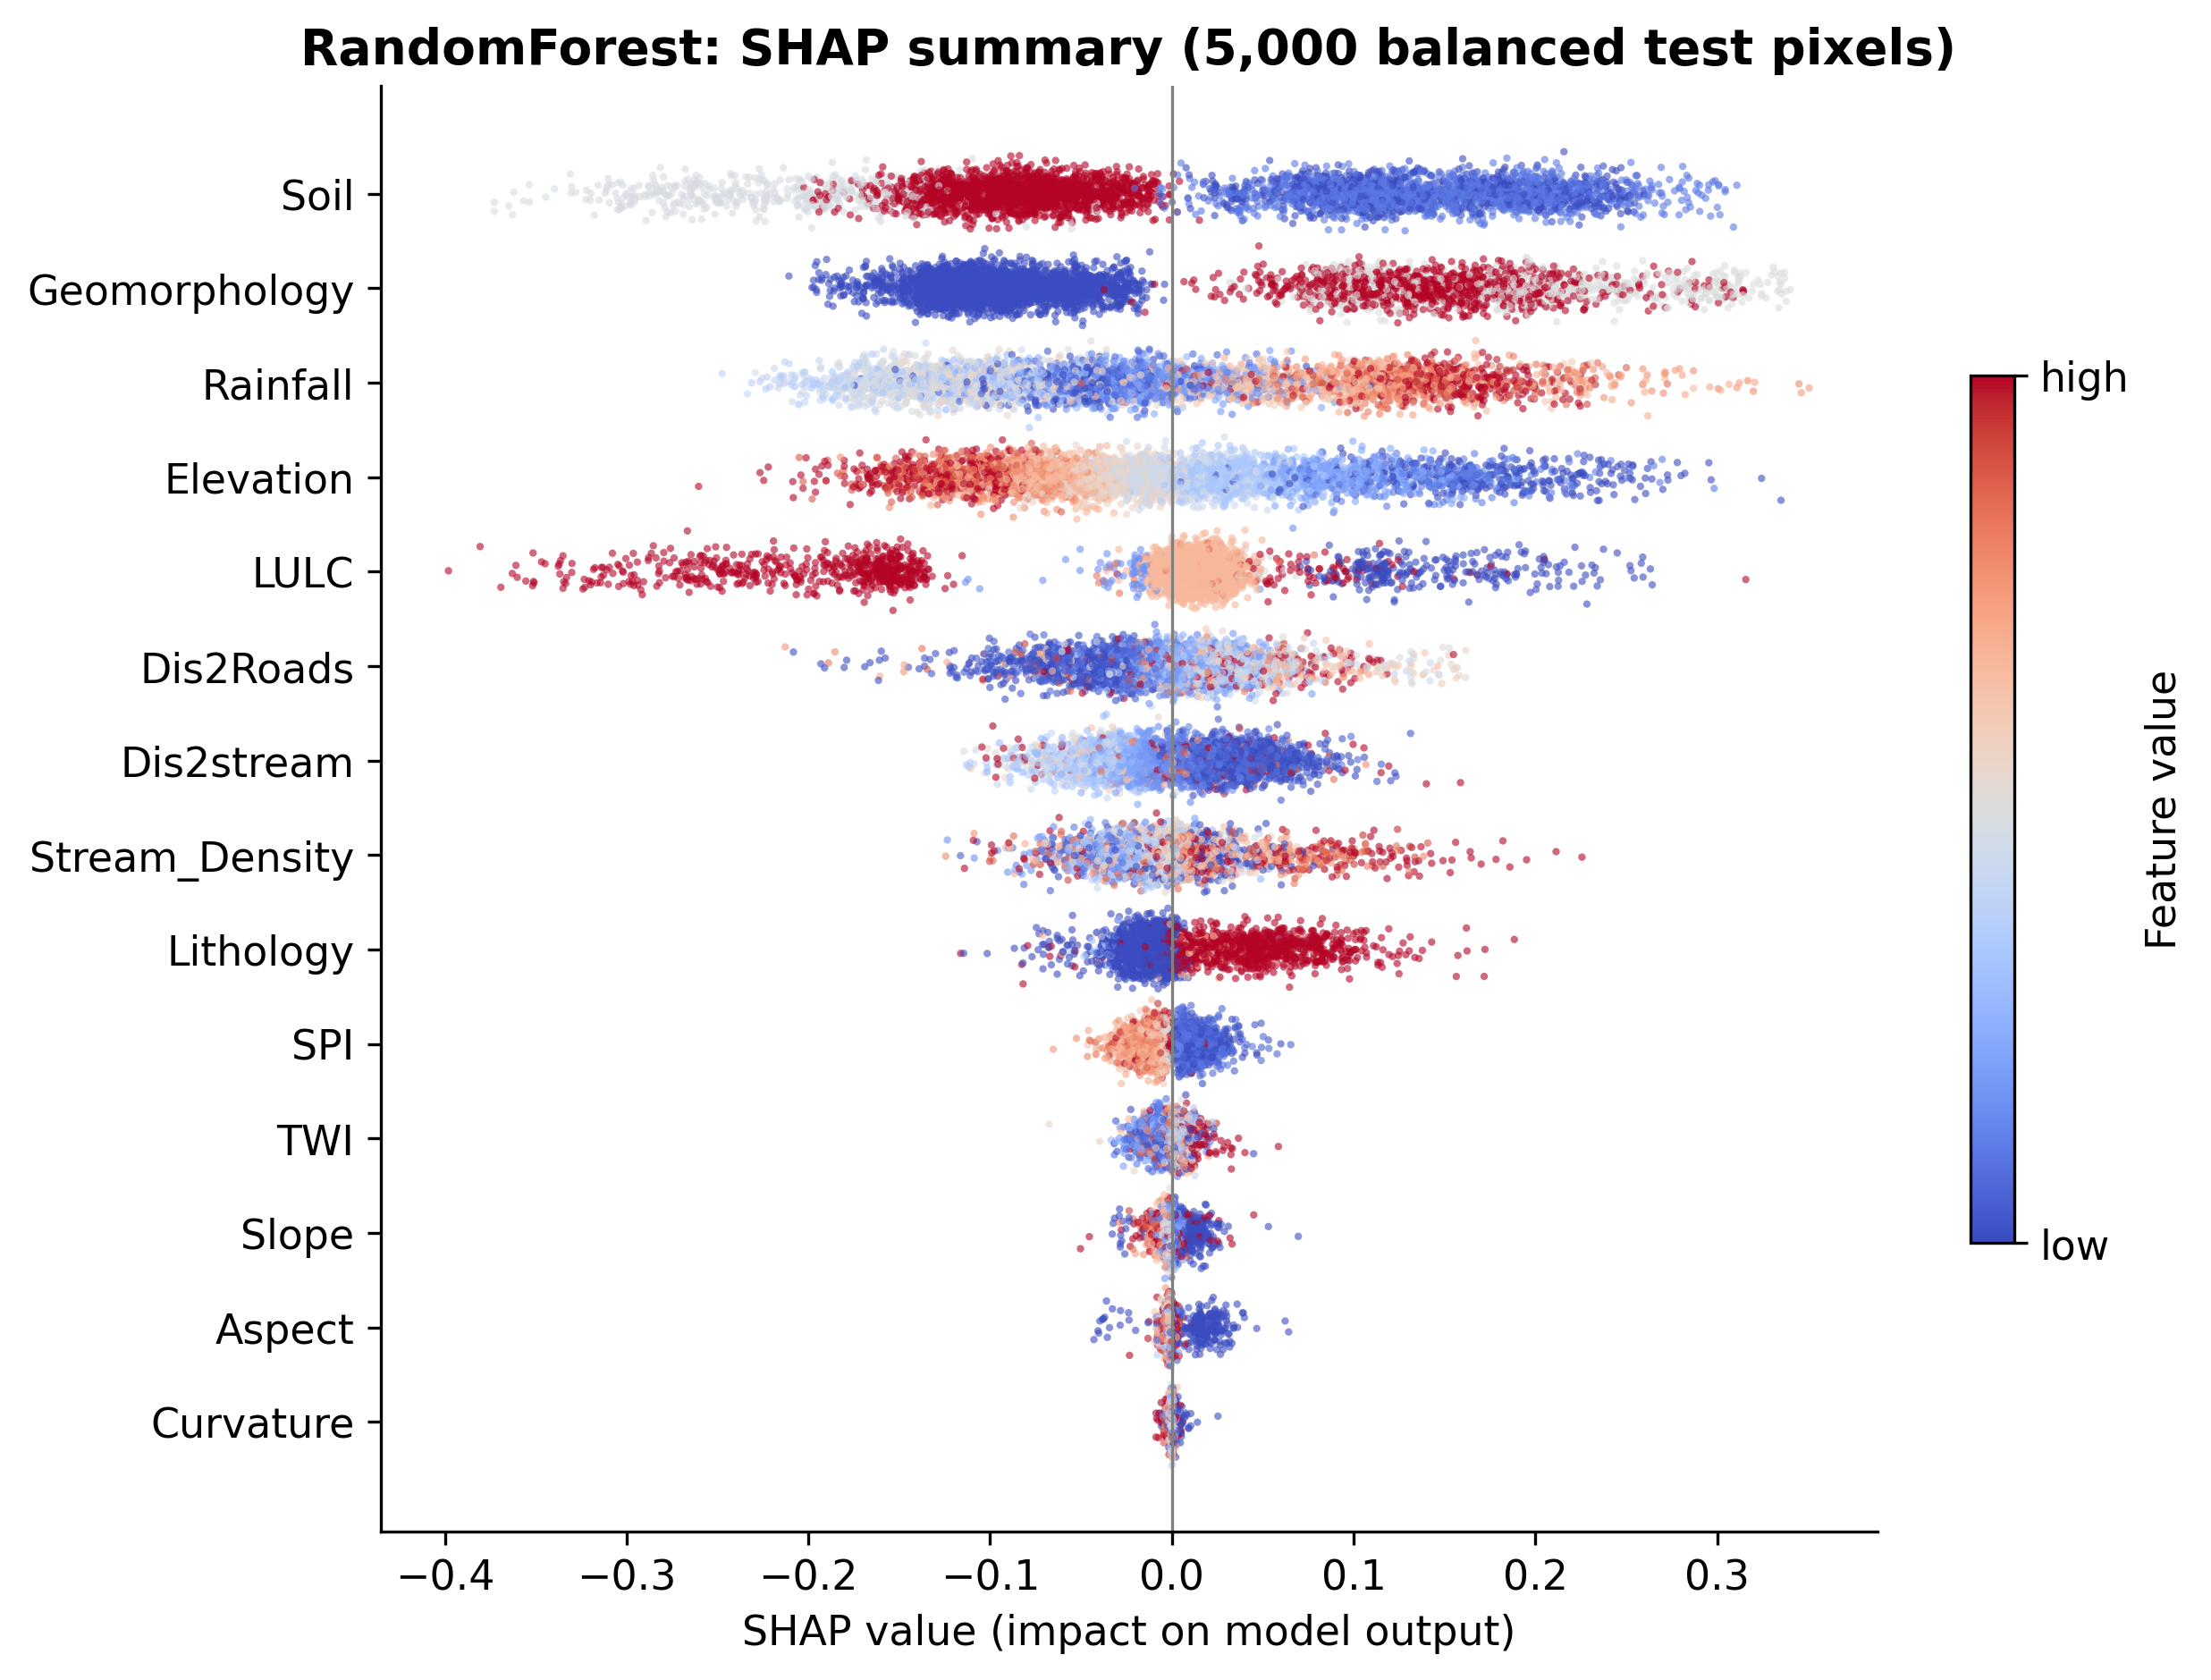
\includegraphics[width=0.85\textwidth]{Figures_v2/Fig_SHAP_Beeswarm_RandomForest.png}
  \caption{RandomForest SHAP beeswarm plot (TreeExplainer on the trained 150-tree forest; values in probability units). Soil ranks first, followed by Geomorphology, Rainfall, and Elevation.}
  \label{fig:shap_beeswarm_rf}
\end{figure}

\begin{figure}[H]
  \centering
  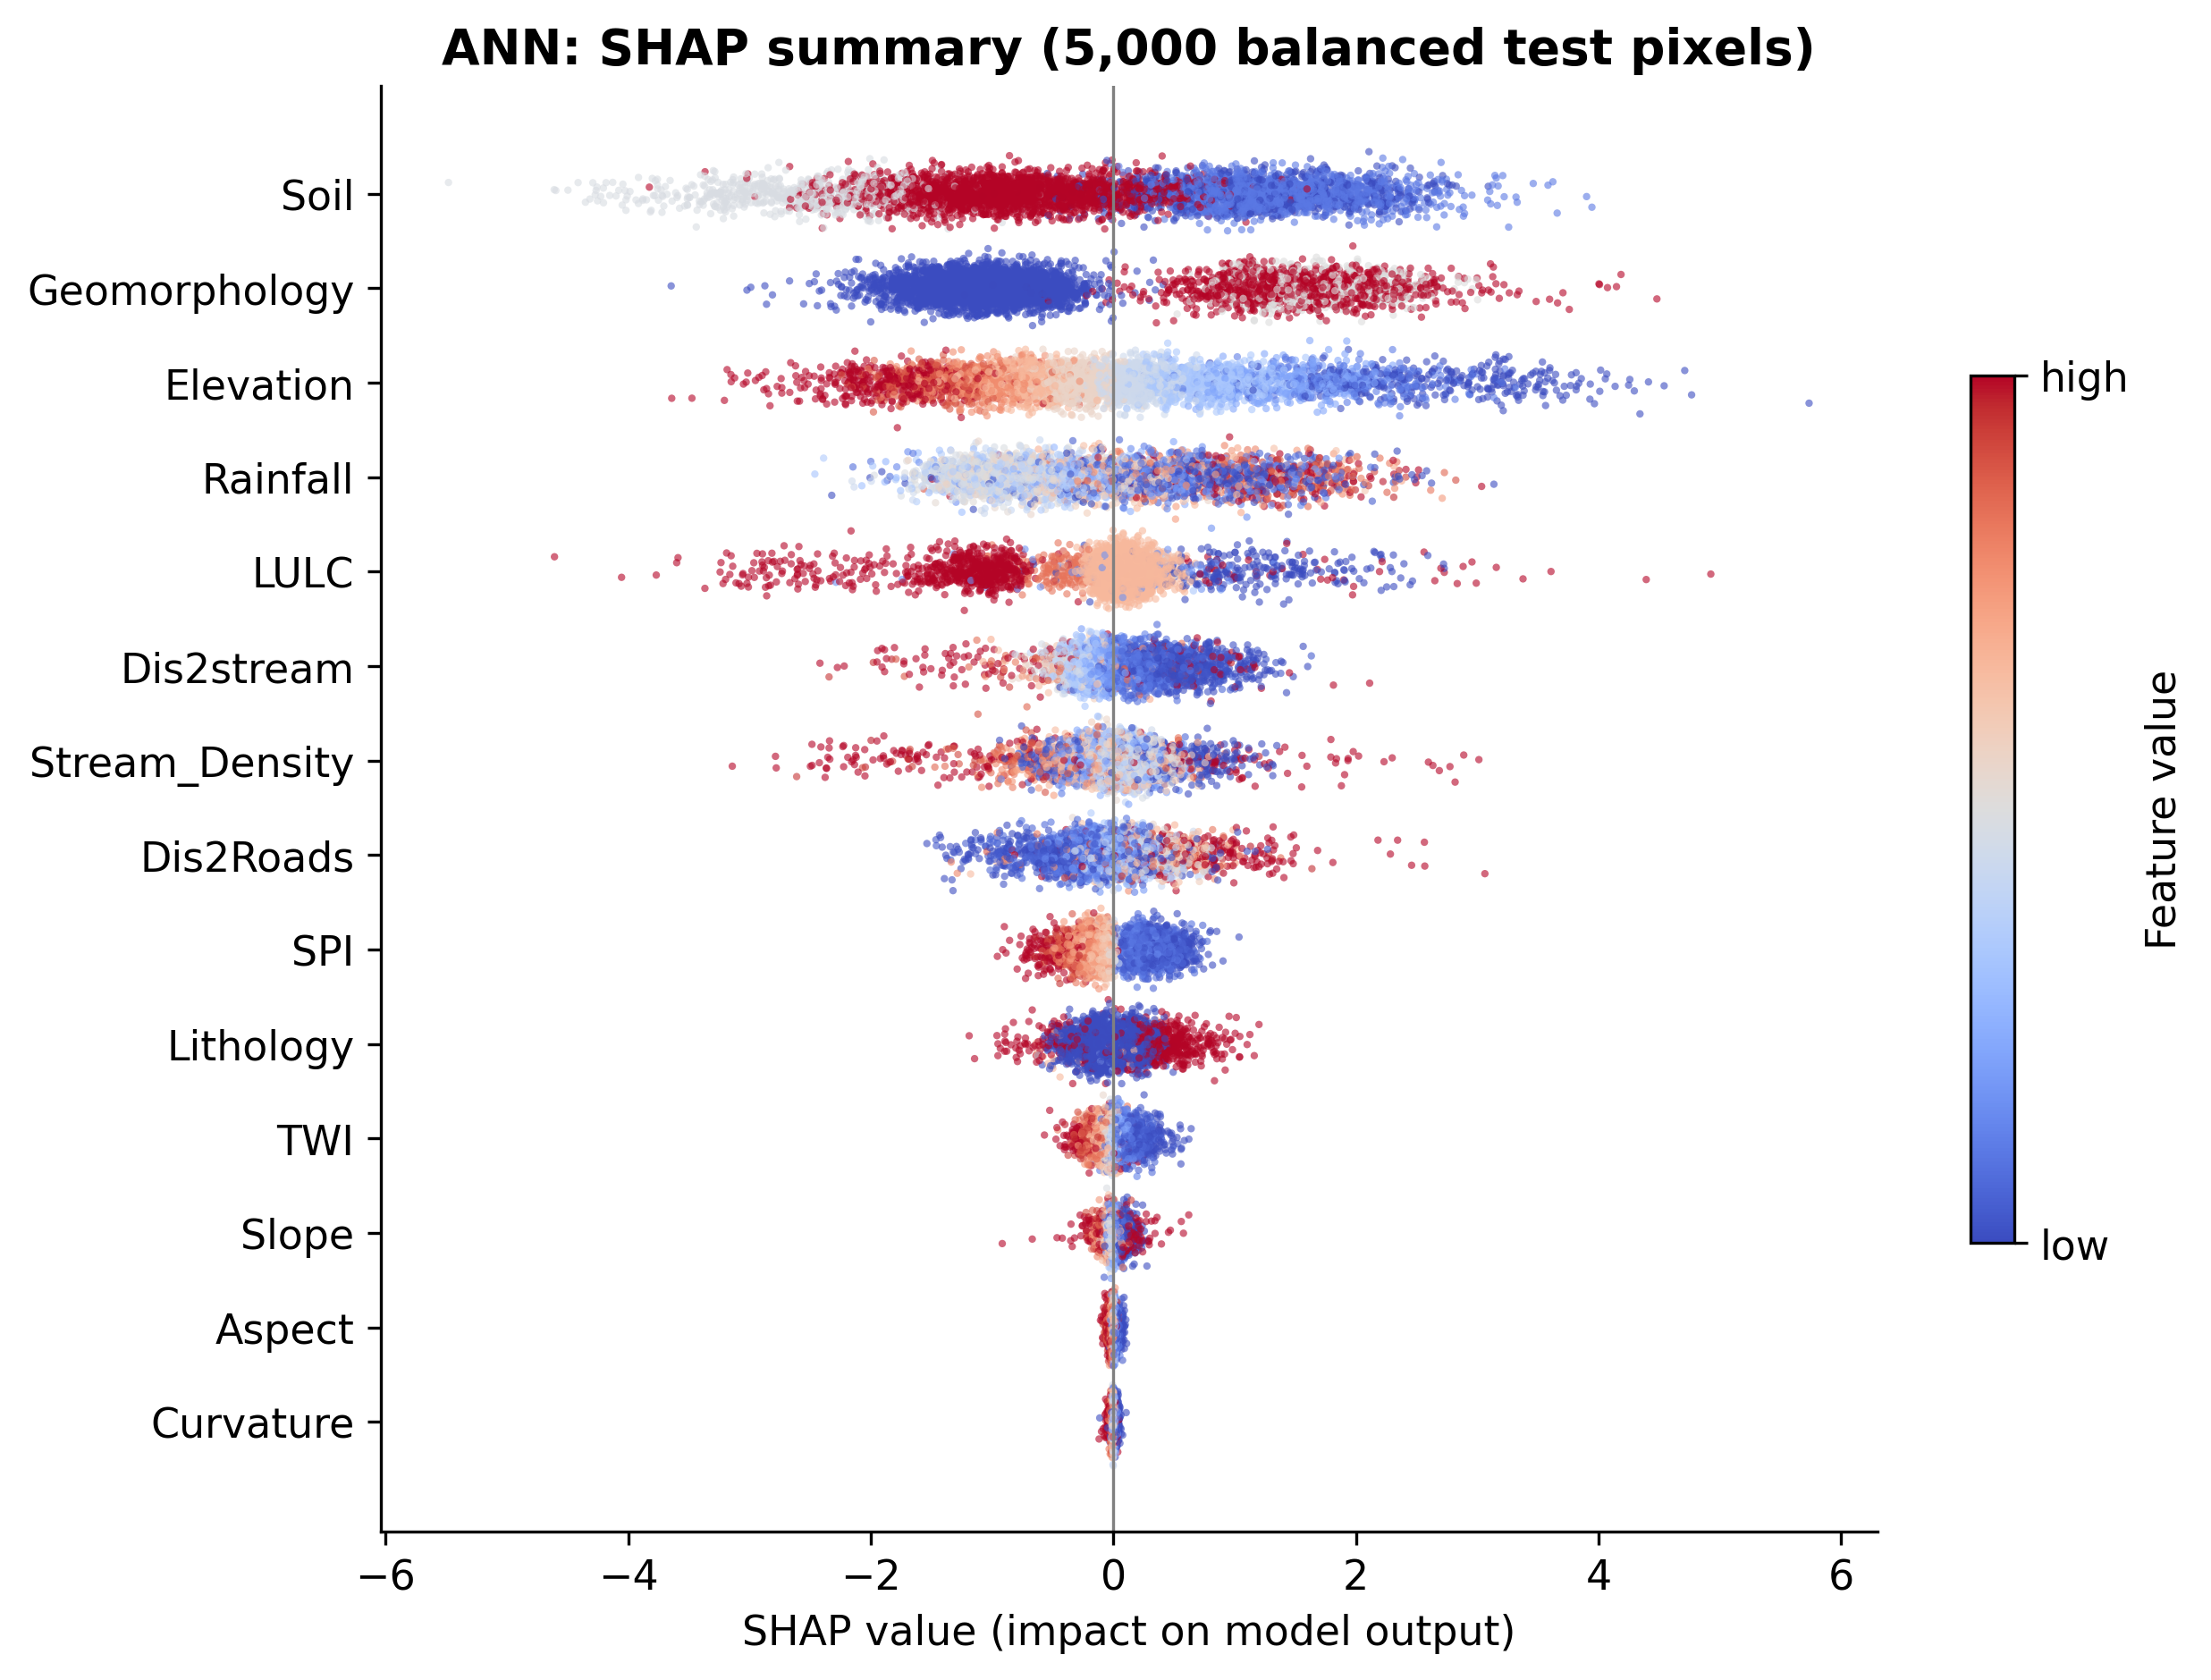
\includegraphics[width=0.85\textwidth]{Figures_v2/Fig_SHAP_Beeswarm_ANN.png}
  \caption{ANN SHAP beeswarm plot (GradientExplainer, all 14 CgFs). Soil, Geomorphology, Elevation, and Rainfall rank 1--4.}
  \label{fig:shap_beeswarm_ann}
\end{figure}

\begin{figure}[H]
  \centering
  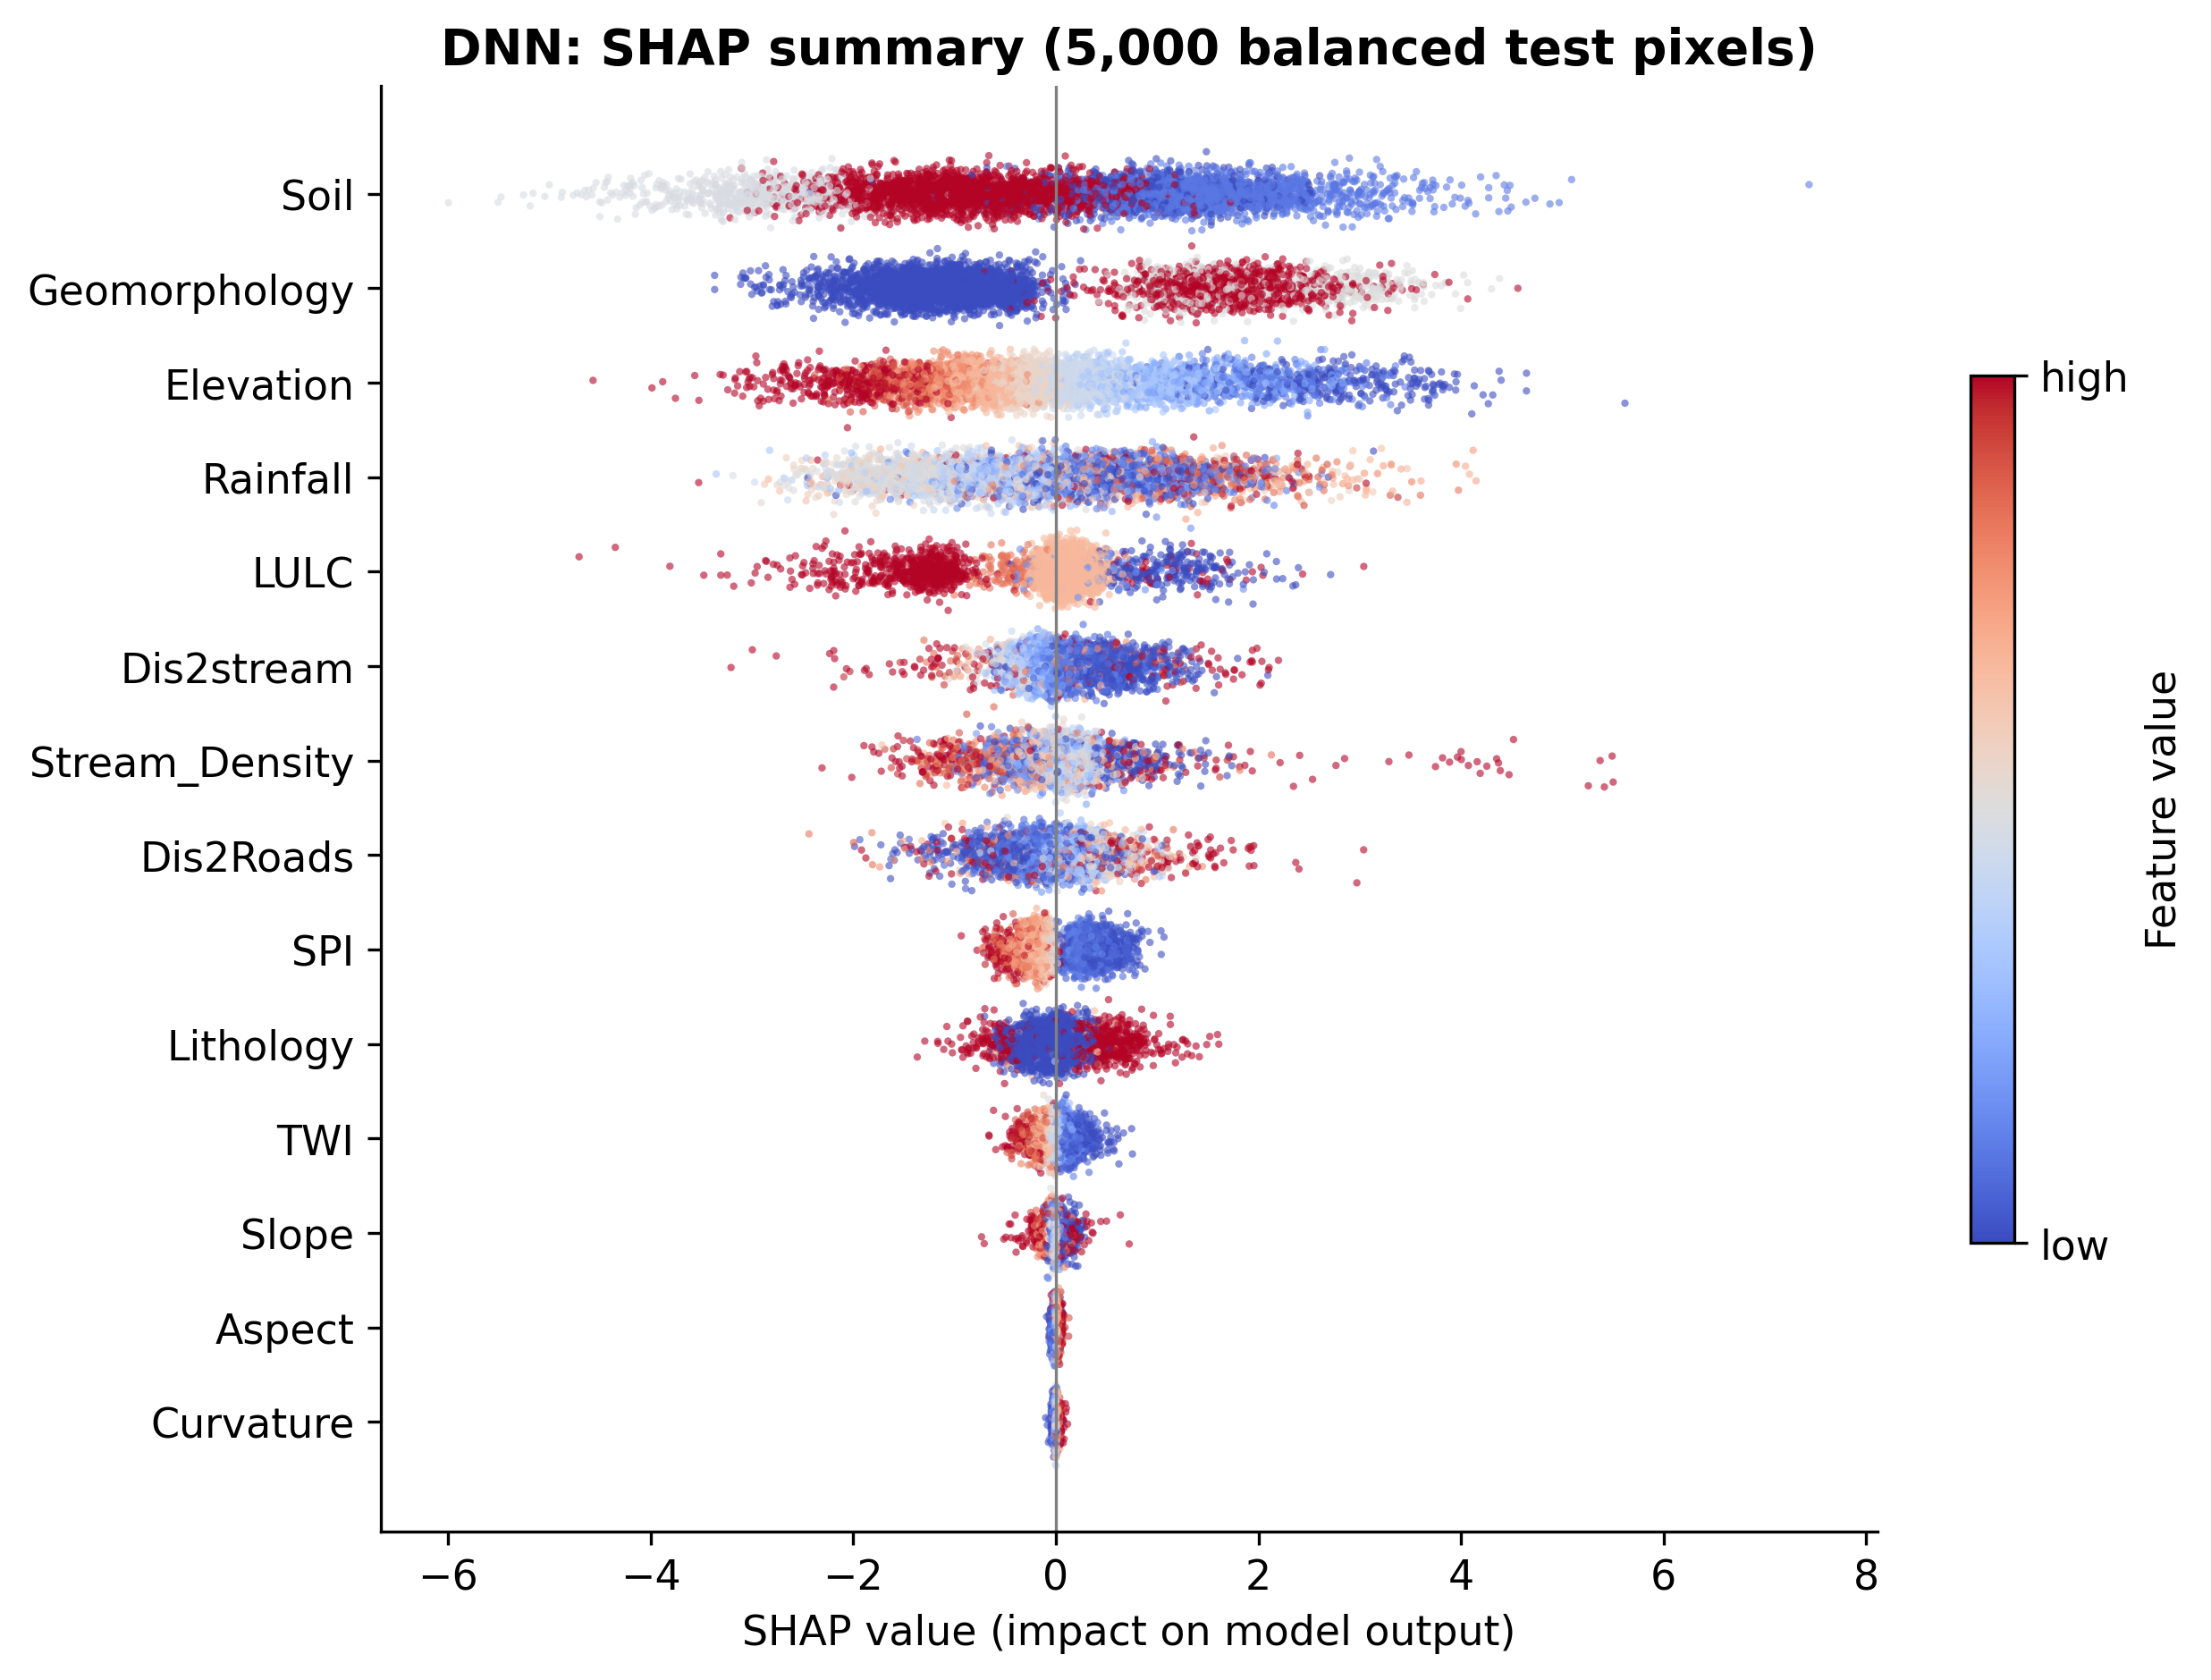
\includegraphics[width=0.85\textwidth]{Figures_v2/Fig_SHAP_Beeswarm_DNN.png}
  \caption{DNN SHAP beeswarm plot (GradientExplainer, all 14 CgFs). The ranking is almost identical to the ANN (Figure~\ref{fig:shap_beeswarm_ann}).}
  \label{fig:shap_beeswarm_dnn}
\end{figure}

\begin{figure}[H]
  \centering
  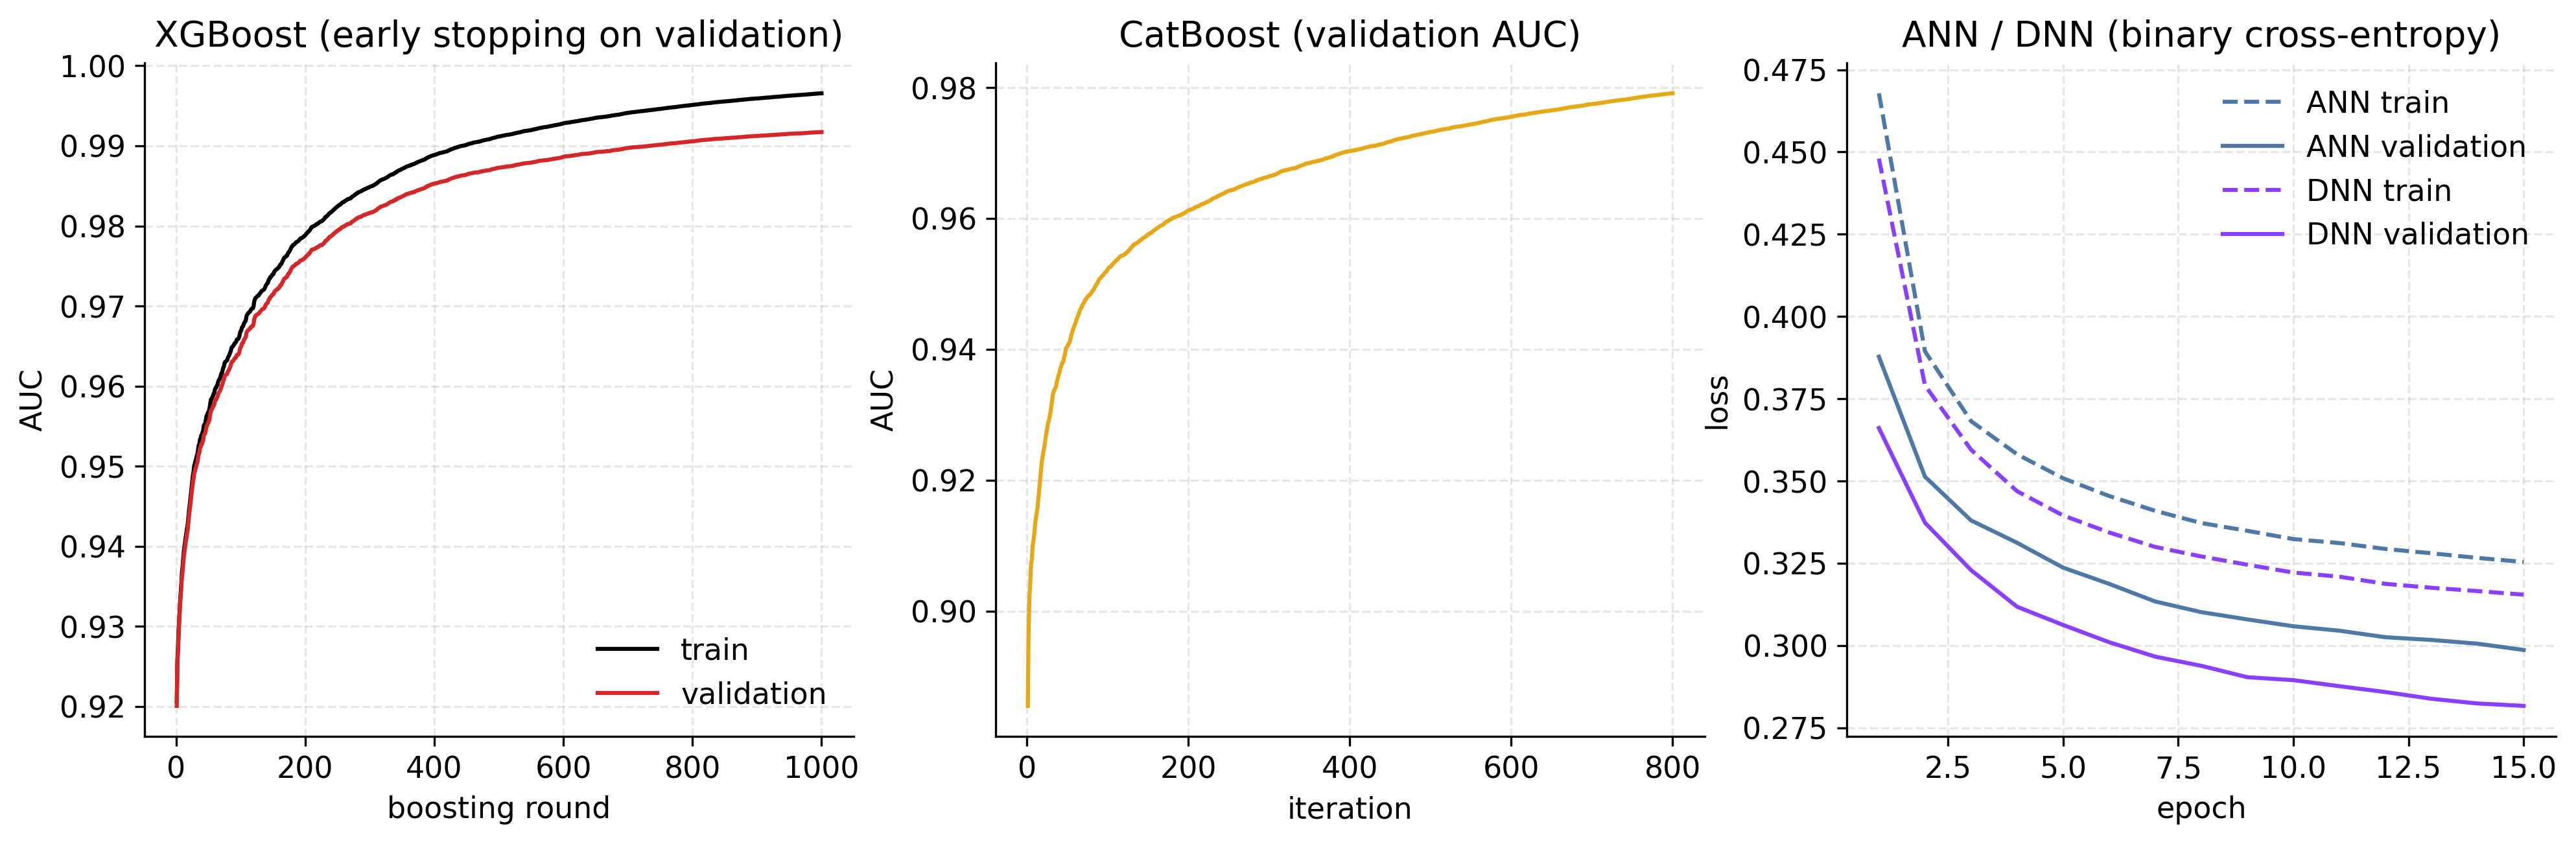
\includegraphics[width=\textwidth]{Figures_v2/Fig_Training_Curves.png}
  \caption{Training histories. Left: XGBoost training and validation AUC per boosting round (early stopping on the validation set did not trigger within 1,000 rounds). Centre: CatBoost validation AUC. Right: ANN and DNN training and validation binary cross-entropy per epoch.}
  \label{fig:training_curves}
\end{figure}

\end{document}
